\documentclass{article}
\usepackage{fullpage}
\usepackage{color}
\usepackage[normalem]{ulem}
\newcommand{\eric}{\textcolor{blue}{[Eric]}}
\newcommand{\richard}{\textcolor{red}{[Richard]}}
\newcommand{\taylor}{\textcolor{green}{[Taylor]}}
\newcommand{\susi}{\textcolor{cyan}{[Susi]}}
\hyphenpenalty=100000
\usepackage{graphicx}
\DeclareGraphicsExtensions{.pdf,.png,.jpg}
\begin{document}
\setlength{\voffset}{3.5in}
\title{Milestone 3}
\author{Team Sriram\\
(Susi Cisneros, Eric Henderson, Taylor Purviance and Richard Thai)}
\date{18 October 2011}
\maketitle
\clearpage
\setlength{\voffset}{0pt}
\tableofcontents
\clearpage
~\\
\begin{Large}\textbf{Changes (based off Git commits)}\end{Large}\\
~\\
\begin{tabular}{ | p{2in} | p{4.5in} | }
\hline
\textbf{Date Time} & \textbf{Description}\\
\hline
\hline
9 October 2011 7:30 pm & Initial version of document\\
\hline
10 October 2011 4:50 pm & Made changes based on input from the client\\
\hline
10 October 2011 6:04 pm & More Milestone 3 changes\\
\hline
10 October 2011 6:41 pm & Added user interface screens to the document\\
\hline
17 October 2011 12:23 pm & Created the rest of the interface screens\\
\hline
17 October 2011 3:36 pm & Added remaining interface screens to document and created commit history\\
\hline
\end{tabular}
\clearpage

\section{Executive Summary}
This milestone, the third of a series, documents the context for a software project proposed by the client, Tim Ekl.  Primarily, this document defines and describers the non-functional requirements such as usability, performance, reliability, supportability, hardware / software interfaces, documentation / installation / legal / licensing, and design constraints requirements.  All of  these requirements are necessary to document since their effects are unobvious in the use cases defined in the second milestone.  In addition, this document contains the user interfaces for a variety of situations in order to provide a better way to enforce the usability requirements prescribed by the client.  This document inherits information from the features, needs, and constraints found in the first milestone and will contribute towards the usability report and the interface designs of the fifth and final milestone.\label{interface}

\section{Introduction}
This document is intended to augment the second milestone, which defined the use cases that satisfied the needs and features of the product, by explaining and elaborating on the nonfunctional requirements and features since use cases focus on user experience.  In addition, the nonfunctional requirements will justify the feature, defined in the second milestone, which was not satisfied by a use case.\\
~\\
In addition, this document will define the usability requirements, performance requirements, reliability requirements, supportability requirements, hardware / software interfaces, documentation / installation / legal / licensing requirements, and design constraints requirements--all of which are defined in the glossary.  The information listed is intended to describe behaviors of the system that are inherent in the use case pre-conditions, use case post-conditions, development phase, and post-development phase.  While not explicitly stated, the nonfunctional requirements encourage a prioritization of code quality over error logging.\\
~\\
Finally, this document inherits information from the first milestone:  needs, features, and constraints.  Furthermore, the information in this document will be utilized in the usability report and the interface designs of the upcoming, fifth milestone.

\section{User Environment}
\begin{itemize}
\item The client uses Chrome [9] whenever possible and prefers that development support Chrome [9] and Firefox [10] browsers.
\item The final product should operate on a Linux server with standard programming languages, programming frameworks, and Apache[11].  Additional packages can be installed if necessary.
\end{itemize}

\section{User Needs}
\begin{tabular}{ | p{0.15in} | p{4.0in} | p{.75in} |}
\hline
\textbf{ID} & \textbf{Need} & \textbf{Priority} \\
\hline
\hline
N0 & Search for parts based off their attributes & Primary \\
\hline
N2 & Identify items via bar codes & Primary \\
\hline
N3 & Keep track of the data associated with an asset & Primary \\
\hline
N4 & Organize search results & Primary \\
\hline
N5 & Insert objects in the system at any point; do not freeze the database & Secondary \\
\hline
N6 & Modify objects; including adding notes to the objects & Secondary \\
\hline
N7 & Access from a second physical location & Optional \\
\hline
N8 & View most-recently acquired asset(s) & Optional \\
\hline
N9 & View a summary of inventory data & Optional \\
\hline
\end{tabular} \\
\textbf{Legend:} \\
Primary - Necessary to the system \\
Secondary - Important to the system \\
Optional - Would be nice to have in the system \\

\section{Features}
\subsection{Feature Listing}
\begin{tabular}{ | p{0.15in} | p{2.0in} | p{0.5in} | p{0.5in} | p{0.5in} | p{0.6in} | p{0.5in} | p{0.65in} | }
\hline
\textbf{ID} & \textbf{Feature}\label{feature} & \textbf{Priority}\label{priority} & \textbf{Effort}\label{effort} & \textbf{Risk}\label{risk} & \textbf{Stability}\label{stability} & \textbf{Target Release}\label{target_release} & \textbf{Assigned To}\label{assigned_to} \\
\hline
\hline
F0 & Online UI & Critical & High & High & Low & 1.0 & Eric \\
\hline
F2 & Add assets to the inventory & Critical & Low & High & Low & 1.0 & Richard \\
\hline
F3 & Modify assets in the inventory & Critical & Low & High & Low & 1.0 & Taylor \\
\hline
F4 & The system keeps track of attributes based on category & Critical & Low & High & Low & 1.0 & Susi \\
\hline
F5 & Use a UPC-A barcode as the unique identifier for each asset\label{upc} & Critical & Low & Medium & Low & 1.0 & Eric \\
\hline
F6 & Provide an updated list of recently-added assets & Useful & Medium & Low & Medium & 1.5 & Richard \\
\hline
F7 & Generate reports of asset inventory & Useful & High & Low & Medium & 2.0 & Taylor \\
\hline
F8 & Sort search results based off of barcode, title, and modified / created timestamp & Useful & High & Low & Low & 2.0 & Susi \\
\hline
F10 & Basic search for items based on name or UPC & Critical & High & High & Low & 1.0 & Eric \\
\hline
F11 & Advanced search for items based on all fields related to the item and its category & Critical & High & High & Low & 1.0 & Richard \\
\hline
F12 & Basic and Advanced searches allow the user to include wildcards in the query & Critical & High & High & Low & 1.0 & Taylor \\
\hline
F13 & Basic and Advanced searches will search first by exact / wildcard match, then by fuzzy match & Critical & High & High & Low & 1.0 & Susi \\
\hline
F14 & REST API & Critical & High & High & Low & 1.0 & Eric \\
\hline
\end{tabular}\label{rest}\\
\textbf{Legend:} \\
Critical - Highest importance \\
Important - Medium importance \\
Useful - Lowest importance \\
High / Medium / Low - Degree of a category \\
1.0 - First release of the system \\
1.5 - Next release of the system with significant changes \\
2.0 - Final release of the system \\
~\\
~\\
\subsection{Feature-to-Need Correspondence}
\begin{tabular}{ | c || c | c | c | c | c | c | c | c | c | c | }
\hline
    & N0 & N2 & N3 & N4 & N5 & N6 & N7 & N8 & N9 \\
\hline
\hline
F0  &    &    &    &    &    &    & X  &    &    \\
\hline
F2  &    &    & X  &    & X  &    &    &    &    \\
\hline
F3  &    &    & X  &    &    & X  &    &    &    \\
\hline
F4  &    &    & X  &    & X  & X  &    &    &    \\
\hline
F5  & X  & X  & X  &    &    &    &    &    &    \\
\hline
F6  &    &    &    &    &    &    &    & X  &    \\
\hline
F7  &    &    &    &    &    &    &    &    & X  \\
\hline
F8  & X  & X  &    & X  &    &    &    &    &    \\
\hline
F10 & X  & X  & X  & X  &    &    &    &    &    \\
\hline
F11 & X  & X  & X  & X  &    &    &    &    &    \\
\hline
F12 & X  & X  & X  & X  &    &    &    &    &    \\
\hline
F13 & X  & X  & X  & X  &    &    &    &    &    \\
\hline
F14 &    &    &    &    &    &    & X  &    &    \\
\hline
\end{tabular}

\section{Client Background}
Tim Ekl is a Rose-Hulman graduate student who possesses a significant amount of computer hardware.  He plans on using this system to be able to quickly and easily locate the equipment he wants to use.  Tim is an experienced developer and plans on maintaining the system after it is finished.  

\section{Current System}
The client does not have a software solution in place.  Currently, Tim has a primitive categorization system in place which involves labeling boxes and then trying to deduce the location of a desired component.  The current system poses a few issues such as not always allowing him to find his items, i.e. there have been instances where an item was found after capital was spent to replace it.

\section{Usability Requirements}
\label{usability}
\textbf{NOTE}: The client will judge the usability of the program
\begin{itemize}
\item User should be able to familiarize himself or herself with the software within one hour
\item An online help system / documentation will not be required
\end{itemize}

\section{Performance Requirements}
\label{performance}
NOTE: Any times described in the Performance Requirements are based on the client's machine specifications, which are: Pentium 4 2.8GHz processor with 1.5GB memory.
\begin{itemize}
\item Searches should take no longer than three seconds
\item There should be no noticeable (as judged by the client) difference in search performance (the most complex task) between 10 items and 1000 items
\item There is no tolerance for any system degradation: the system is either fully functional or not functional at all, and there is no need to handle failures.\label{degrad_sys}
\end{itemize}

\section{Reliability Requirements}
\label{reliability}
\begin{itemize}
\item The system should not be down more than once every two months
\item The system repair will be the responsibility of the client after the product is delivered
\item The system must have no data corruption (100\% accuracy)\label{data_corruption}
\item The system will have no more than two bugs per thousand lines of code\label{bug}
\item The system should minimize the number of critical bugs, though there is no defined threshold
\end{itemize}

\section{Supportability Requirements}
\label{support}
\begin{itemize}
\item The system should be able to be supported by open source community and the client
\item The source code needs to be kept clean and easy to understand
\item The source code will follow Ruby coding standards and naming conventions
\item The client should be able to extend the system with features of moderate complexity within four hours; this is an intended effect from following the Ruby coding standards
\item The source code should be as modular as possible in order to simplify extension
\item Adding / modifying an API route should as difficult as adding / modifying a web application feature of equal complexity
\end{itemize}

\section{Hardware and Software Interfaces}
The final product will utilize and / or be compatible with the following software products:\\
\begin{itemize}
\item Ruby 1.9.2 [2]
\item Sinatra 1.3.0 [3]
\item Ubuntu 11.04 [4]
\item SQLite 3.7.8 [5]
\item Cucumber 1.1.0 [6]
\item RSpec 2.6.0 [7]
\item DataMapper 1.1.0 [8]
\item Google Chrome 14.0.8 [9]
\item Firefox 7.0.1 [10]
\item Apache 2.2 [11]
\end{itemize}

\section{Documentation, Installation, Legal, and Licensing Requirements}
\begin{itemize}
\item The project should be open source, distributed under the BSD license
\item Copyright ownership will be given to the client
\item Installation should only require installing the necessary packages and pulling the code from the Git repository into the web server directory
\item The only documentation necessary is a simple readme as well as comments near complex sections of code
\end{itemize}

\section{Design Constraints}
\begin{itemize}
\item The project must be open source
\item The project must be completed within five months
\item The project must be completed without funding from the client
\item The project must utilize REST, not SOAP\label{soap}
\item Develop in Ruby utilizing Sinatra for web framework
\item Accessible via the web.
\end{itemize} 

\section{User Interfaces}
\graphicspath{{../StoryboardImages/}}
~\\
\begin{tabular}{ p{4.5in} }
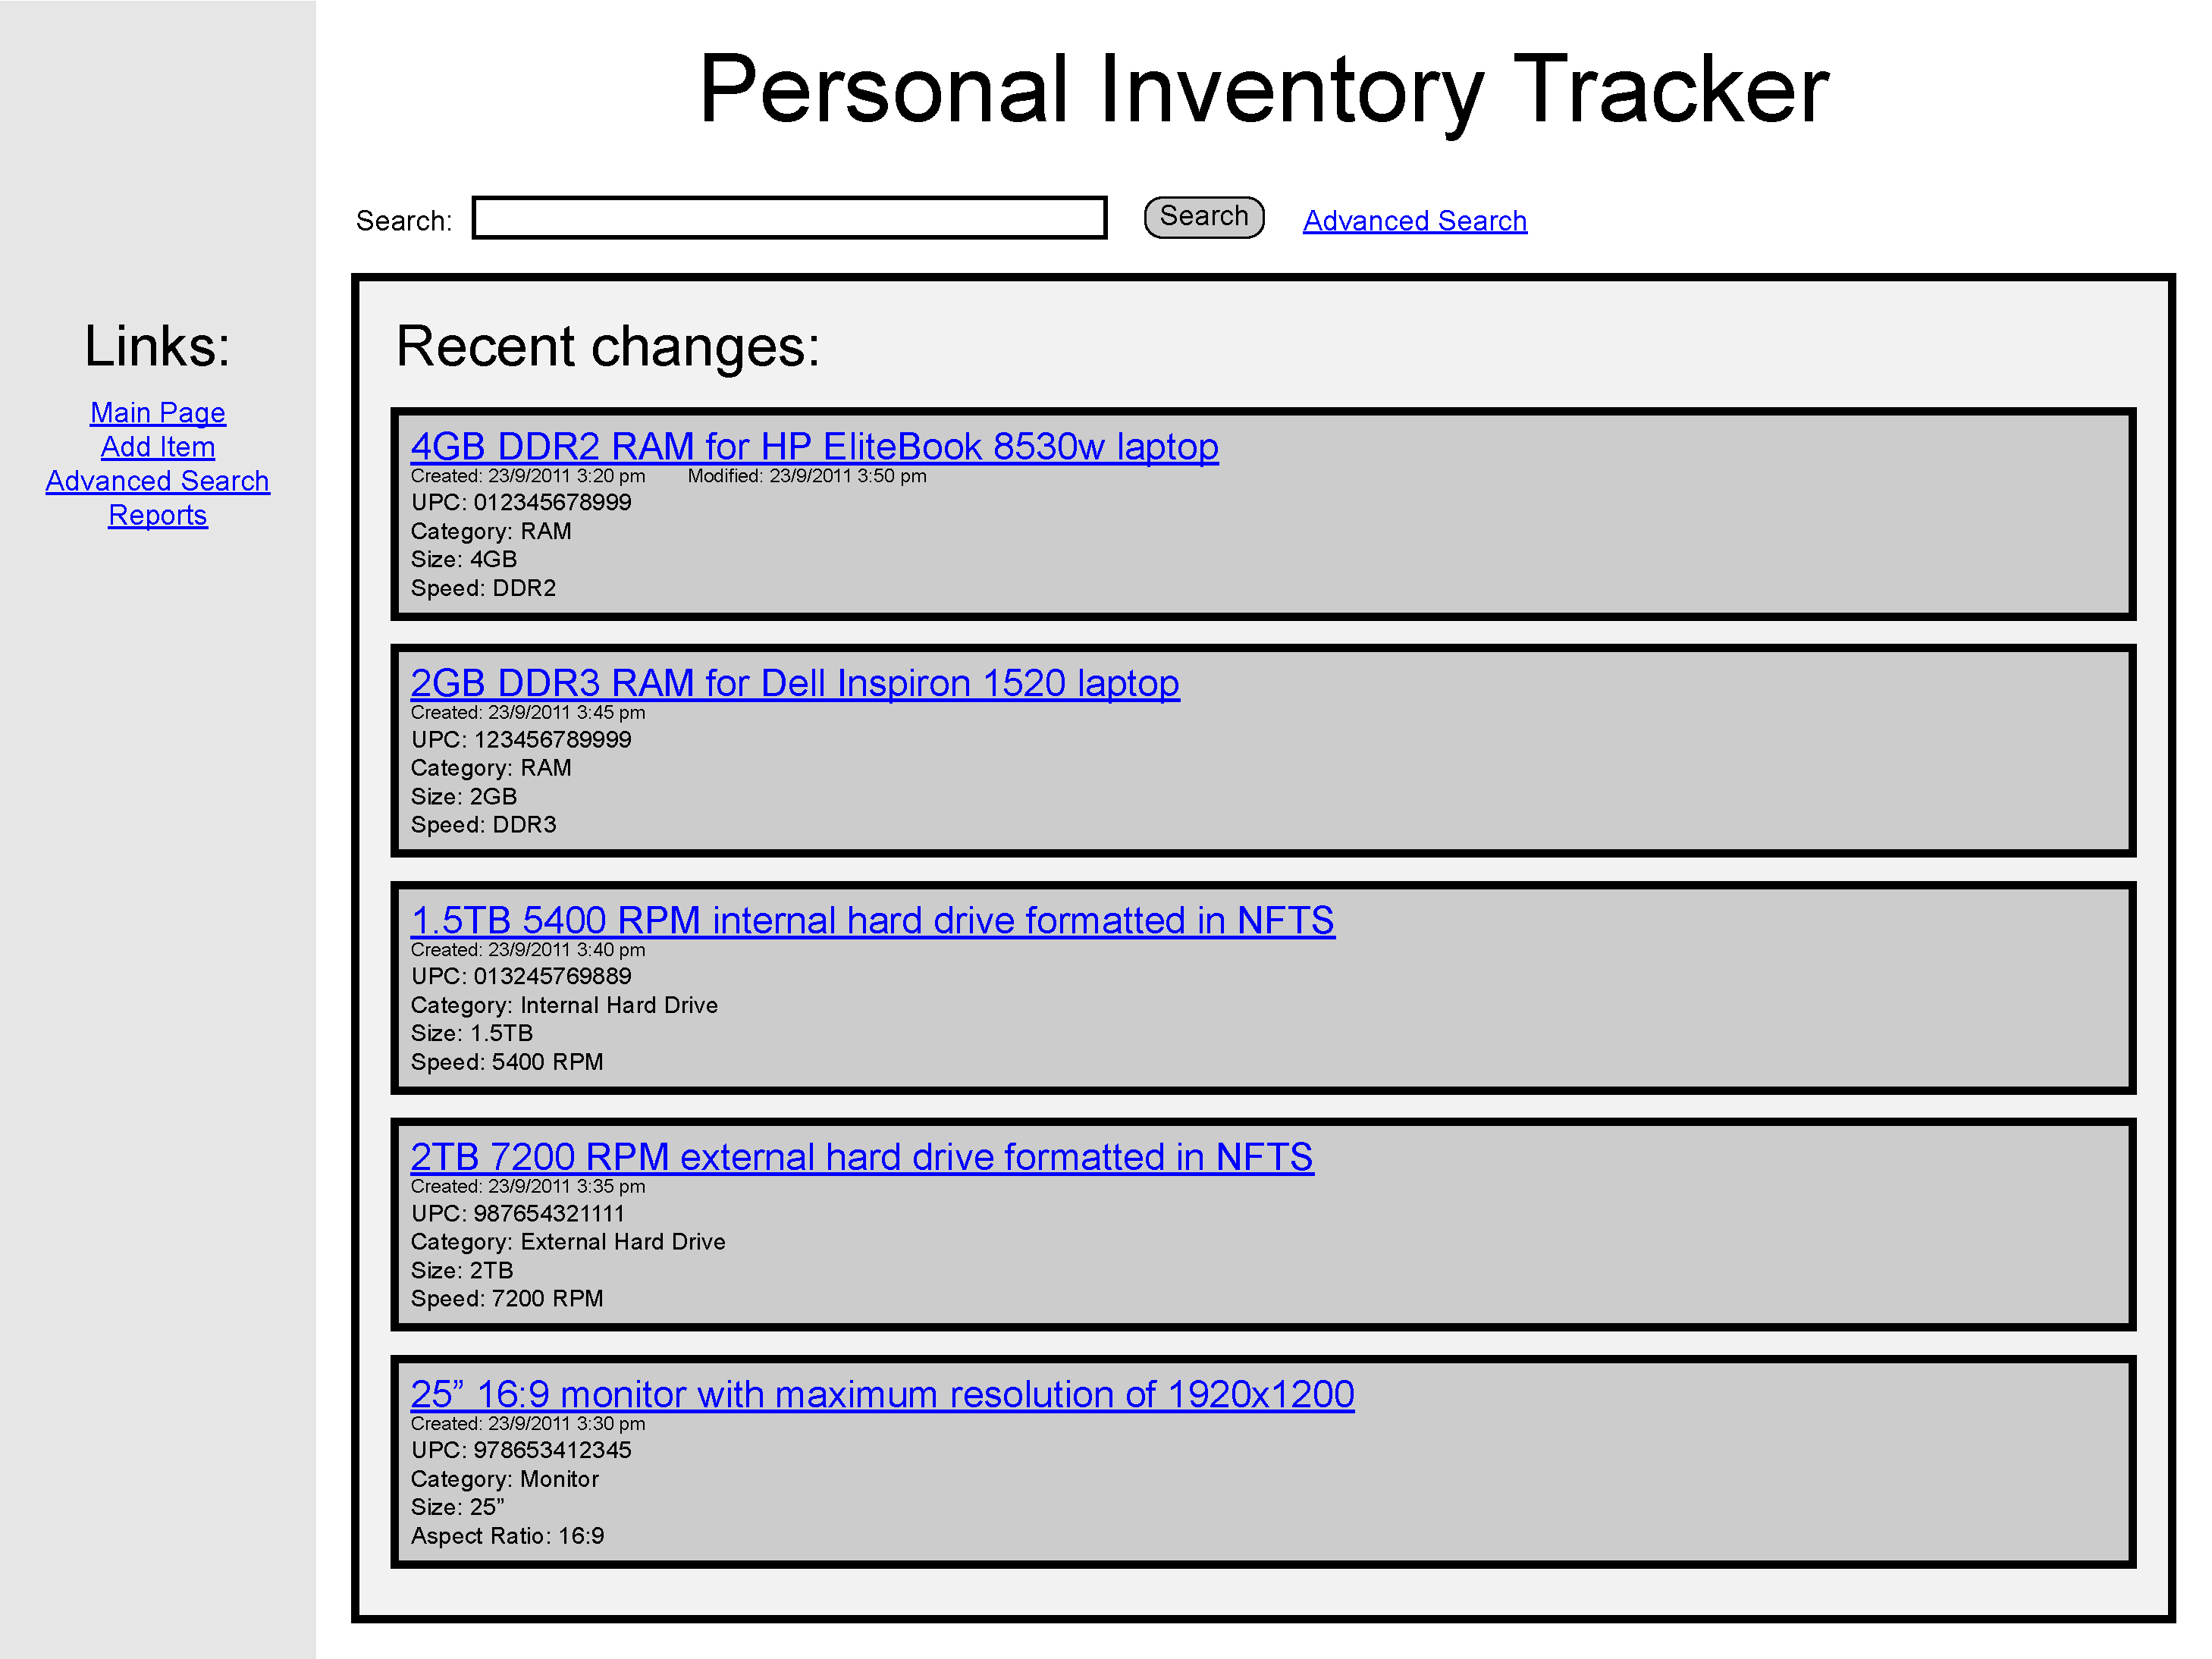
\includegraphics[keepaspectratio, width=4.5in]{addItemF0S0.pdf}\\
The main page
\end{tabular}\\
~\\
~\\
\begin{tabular}{ p{4.5in} }
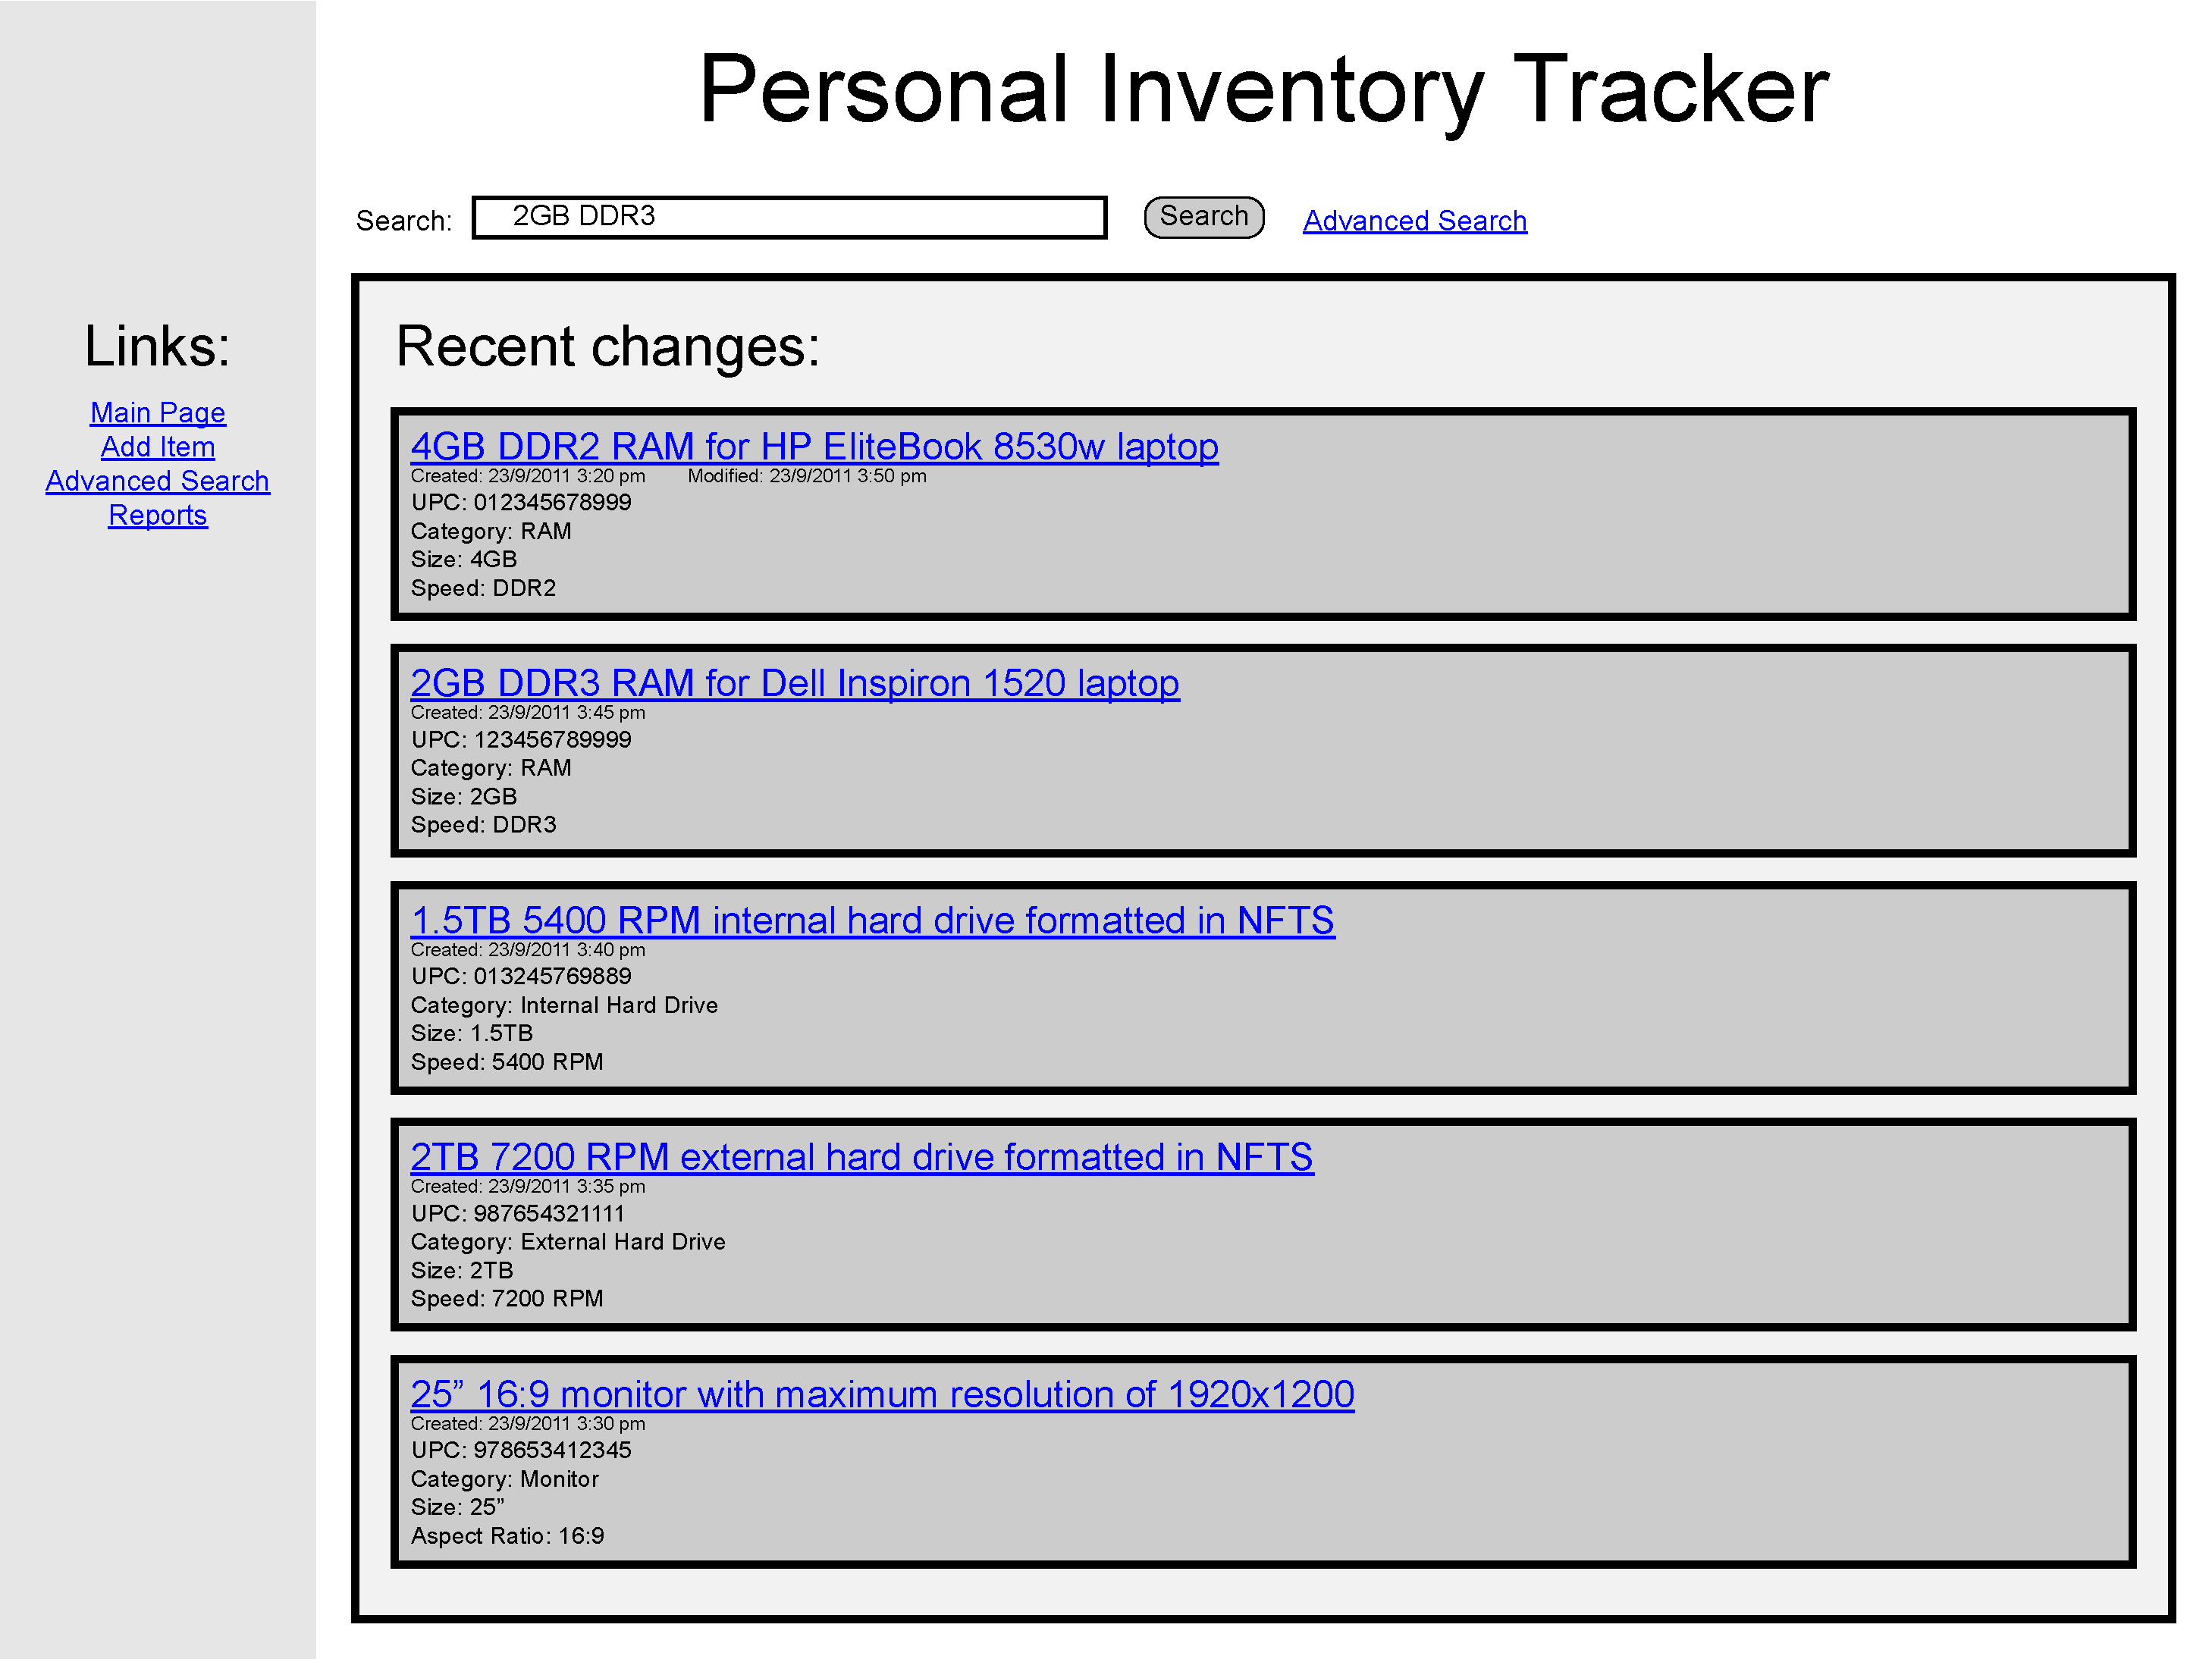
\includegraphics[keepaspectratio, width=4.5in]{basicSearchF0S0.pdf} \\
The main page with a basic search query filled in
\end{tabular}\\
~\\
~\\
\begin{tabular}{ p{4.5in} }
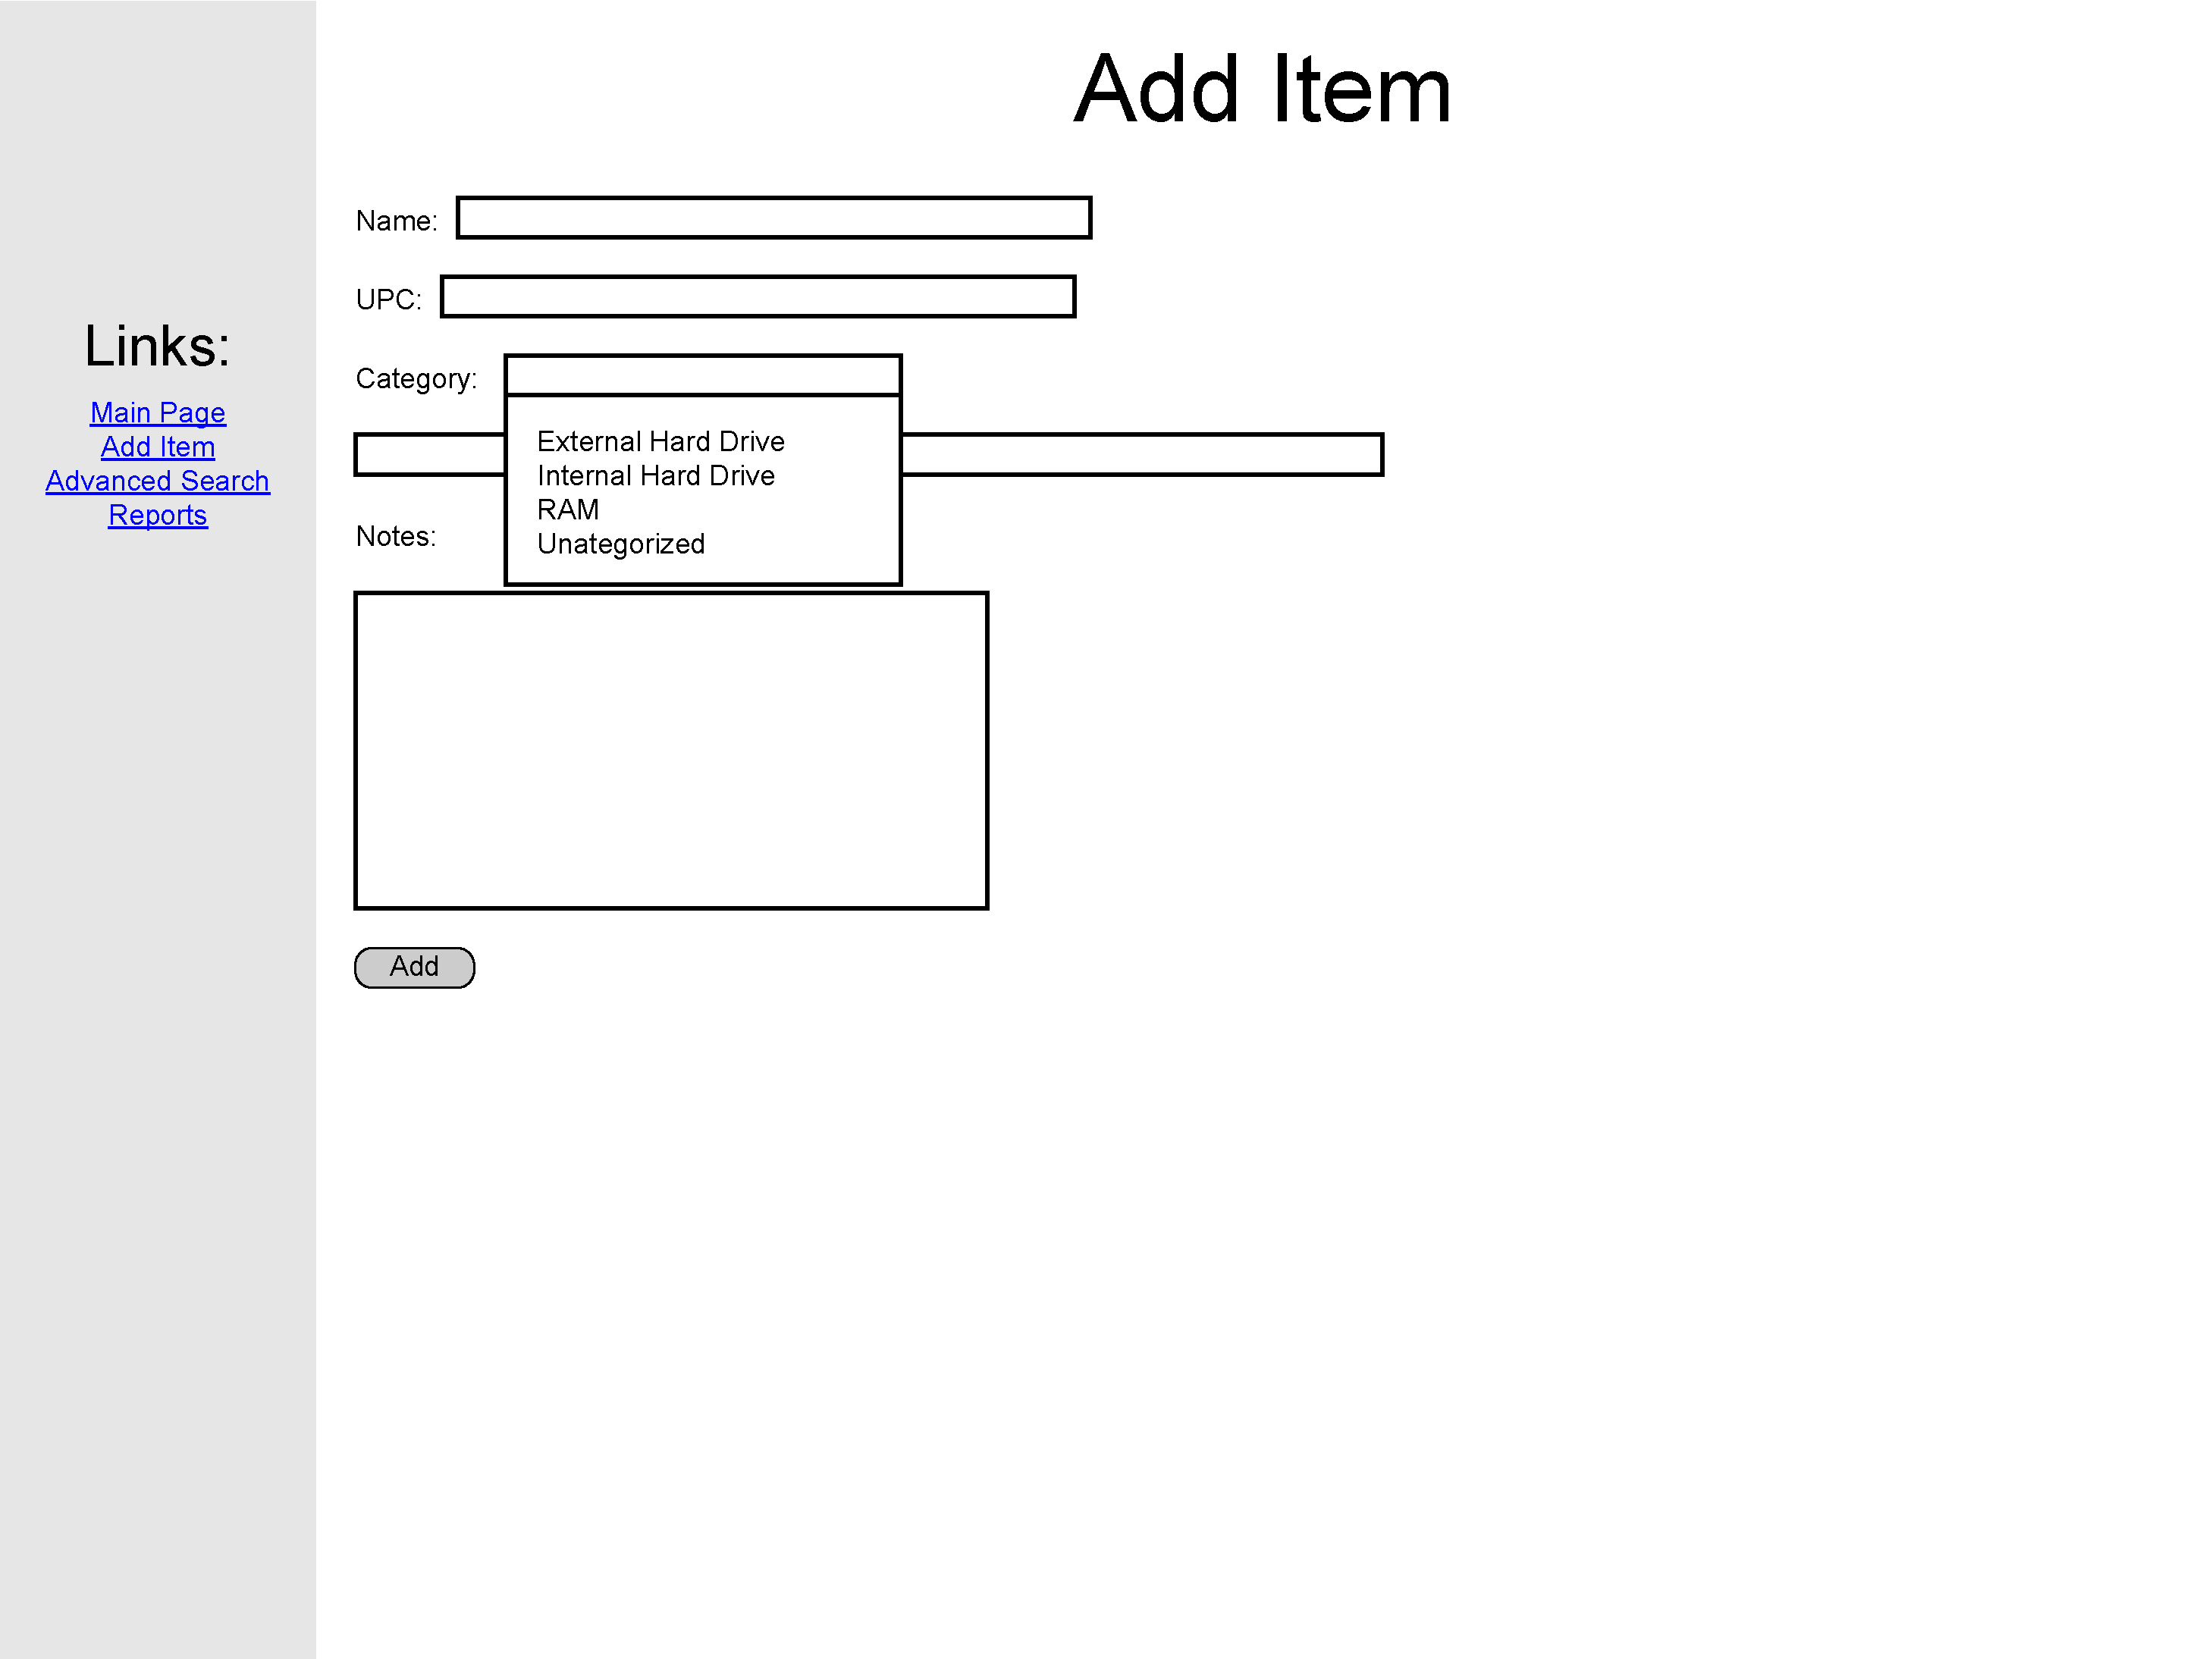
\includegraphics[keepaspectratio, width=4.5in]{addItemF0S1.pdf}\\
The add item page with category autocomplete showing
\end{tabular}\\
~\\
~\\
\begin{tabular}{ p{4.5in} }
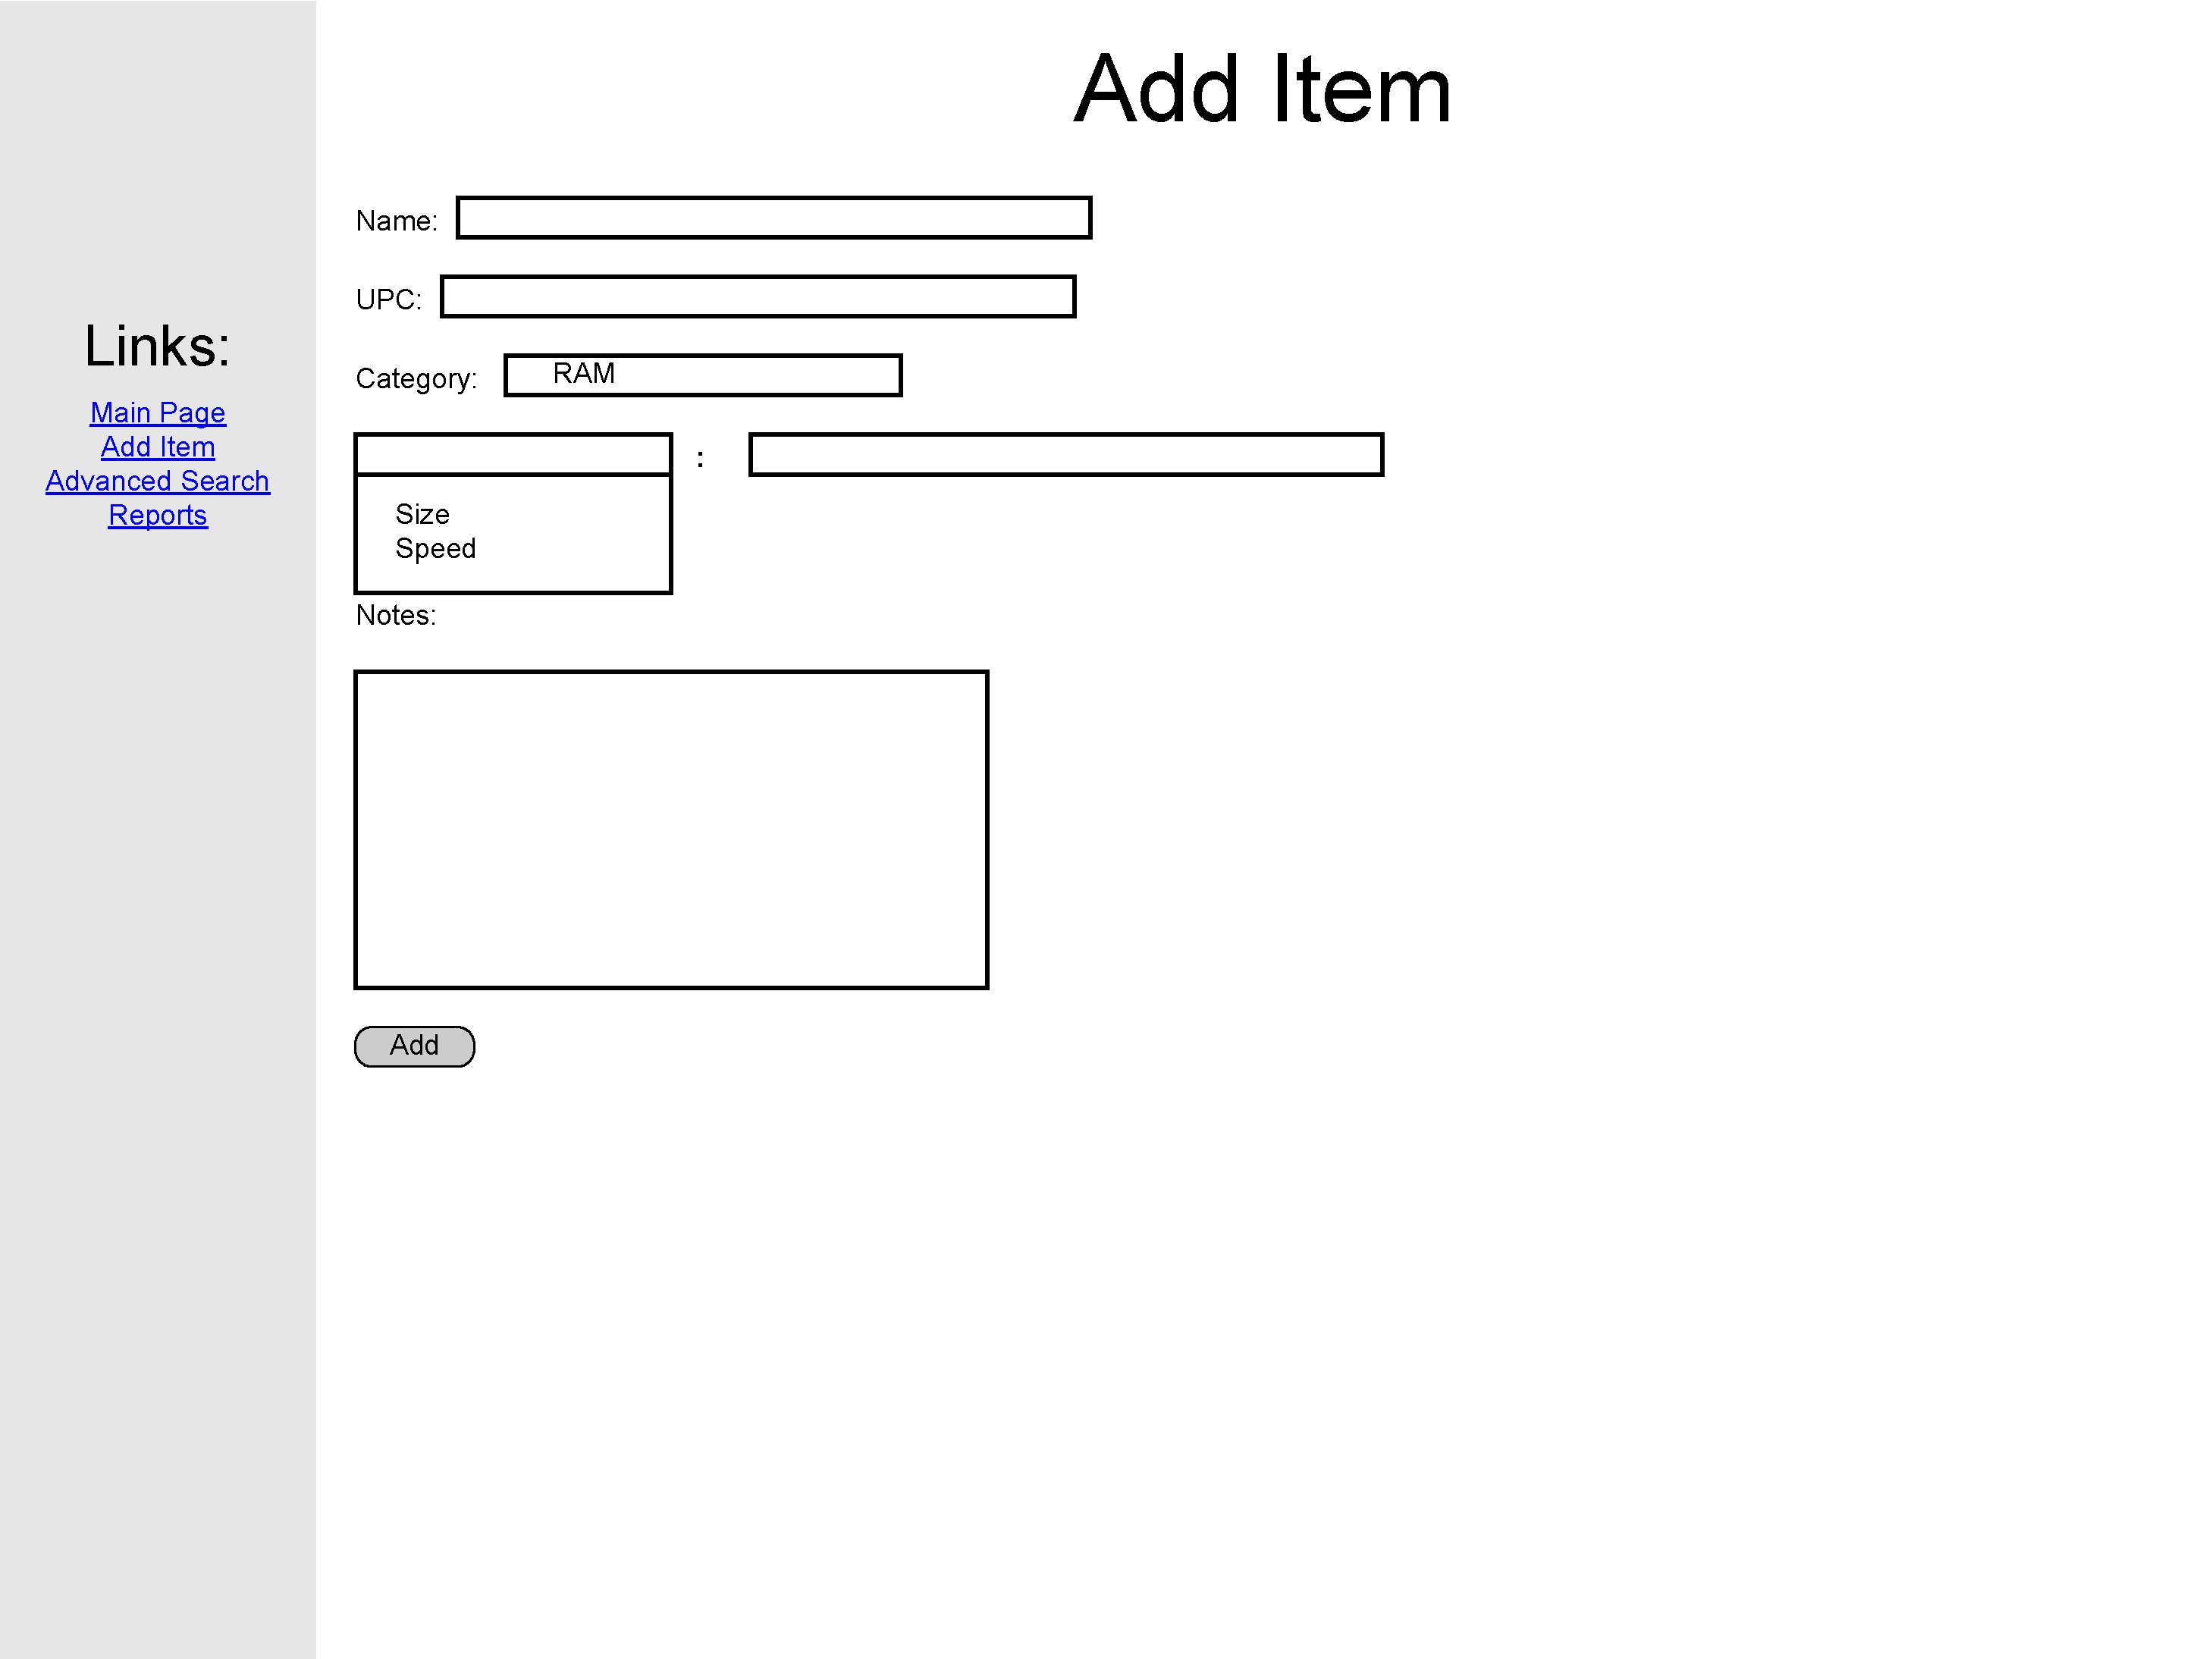
\includegraphics[keepaspectratio, width=4.5in]{addItemF0S2.pdf}  \\
The add item page with category selected and attribute autocomplete showing
\end{tabular}\\
~\\
~\\
\begin{tabular}{ p{4.5in} }
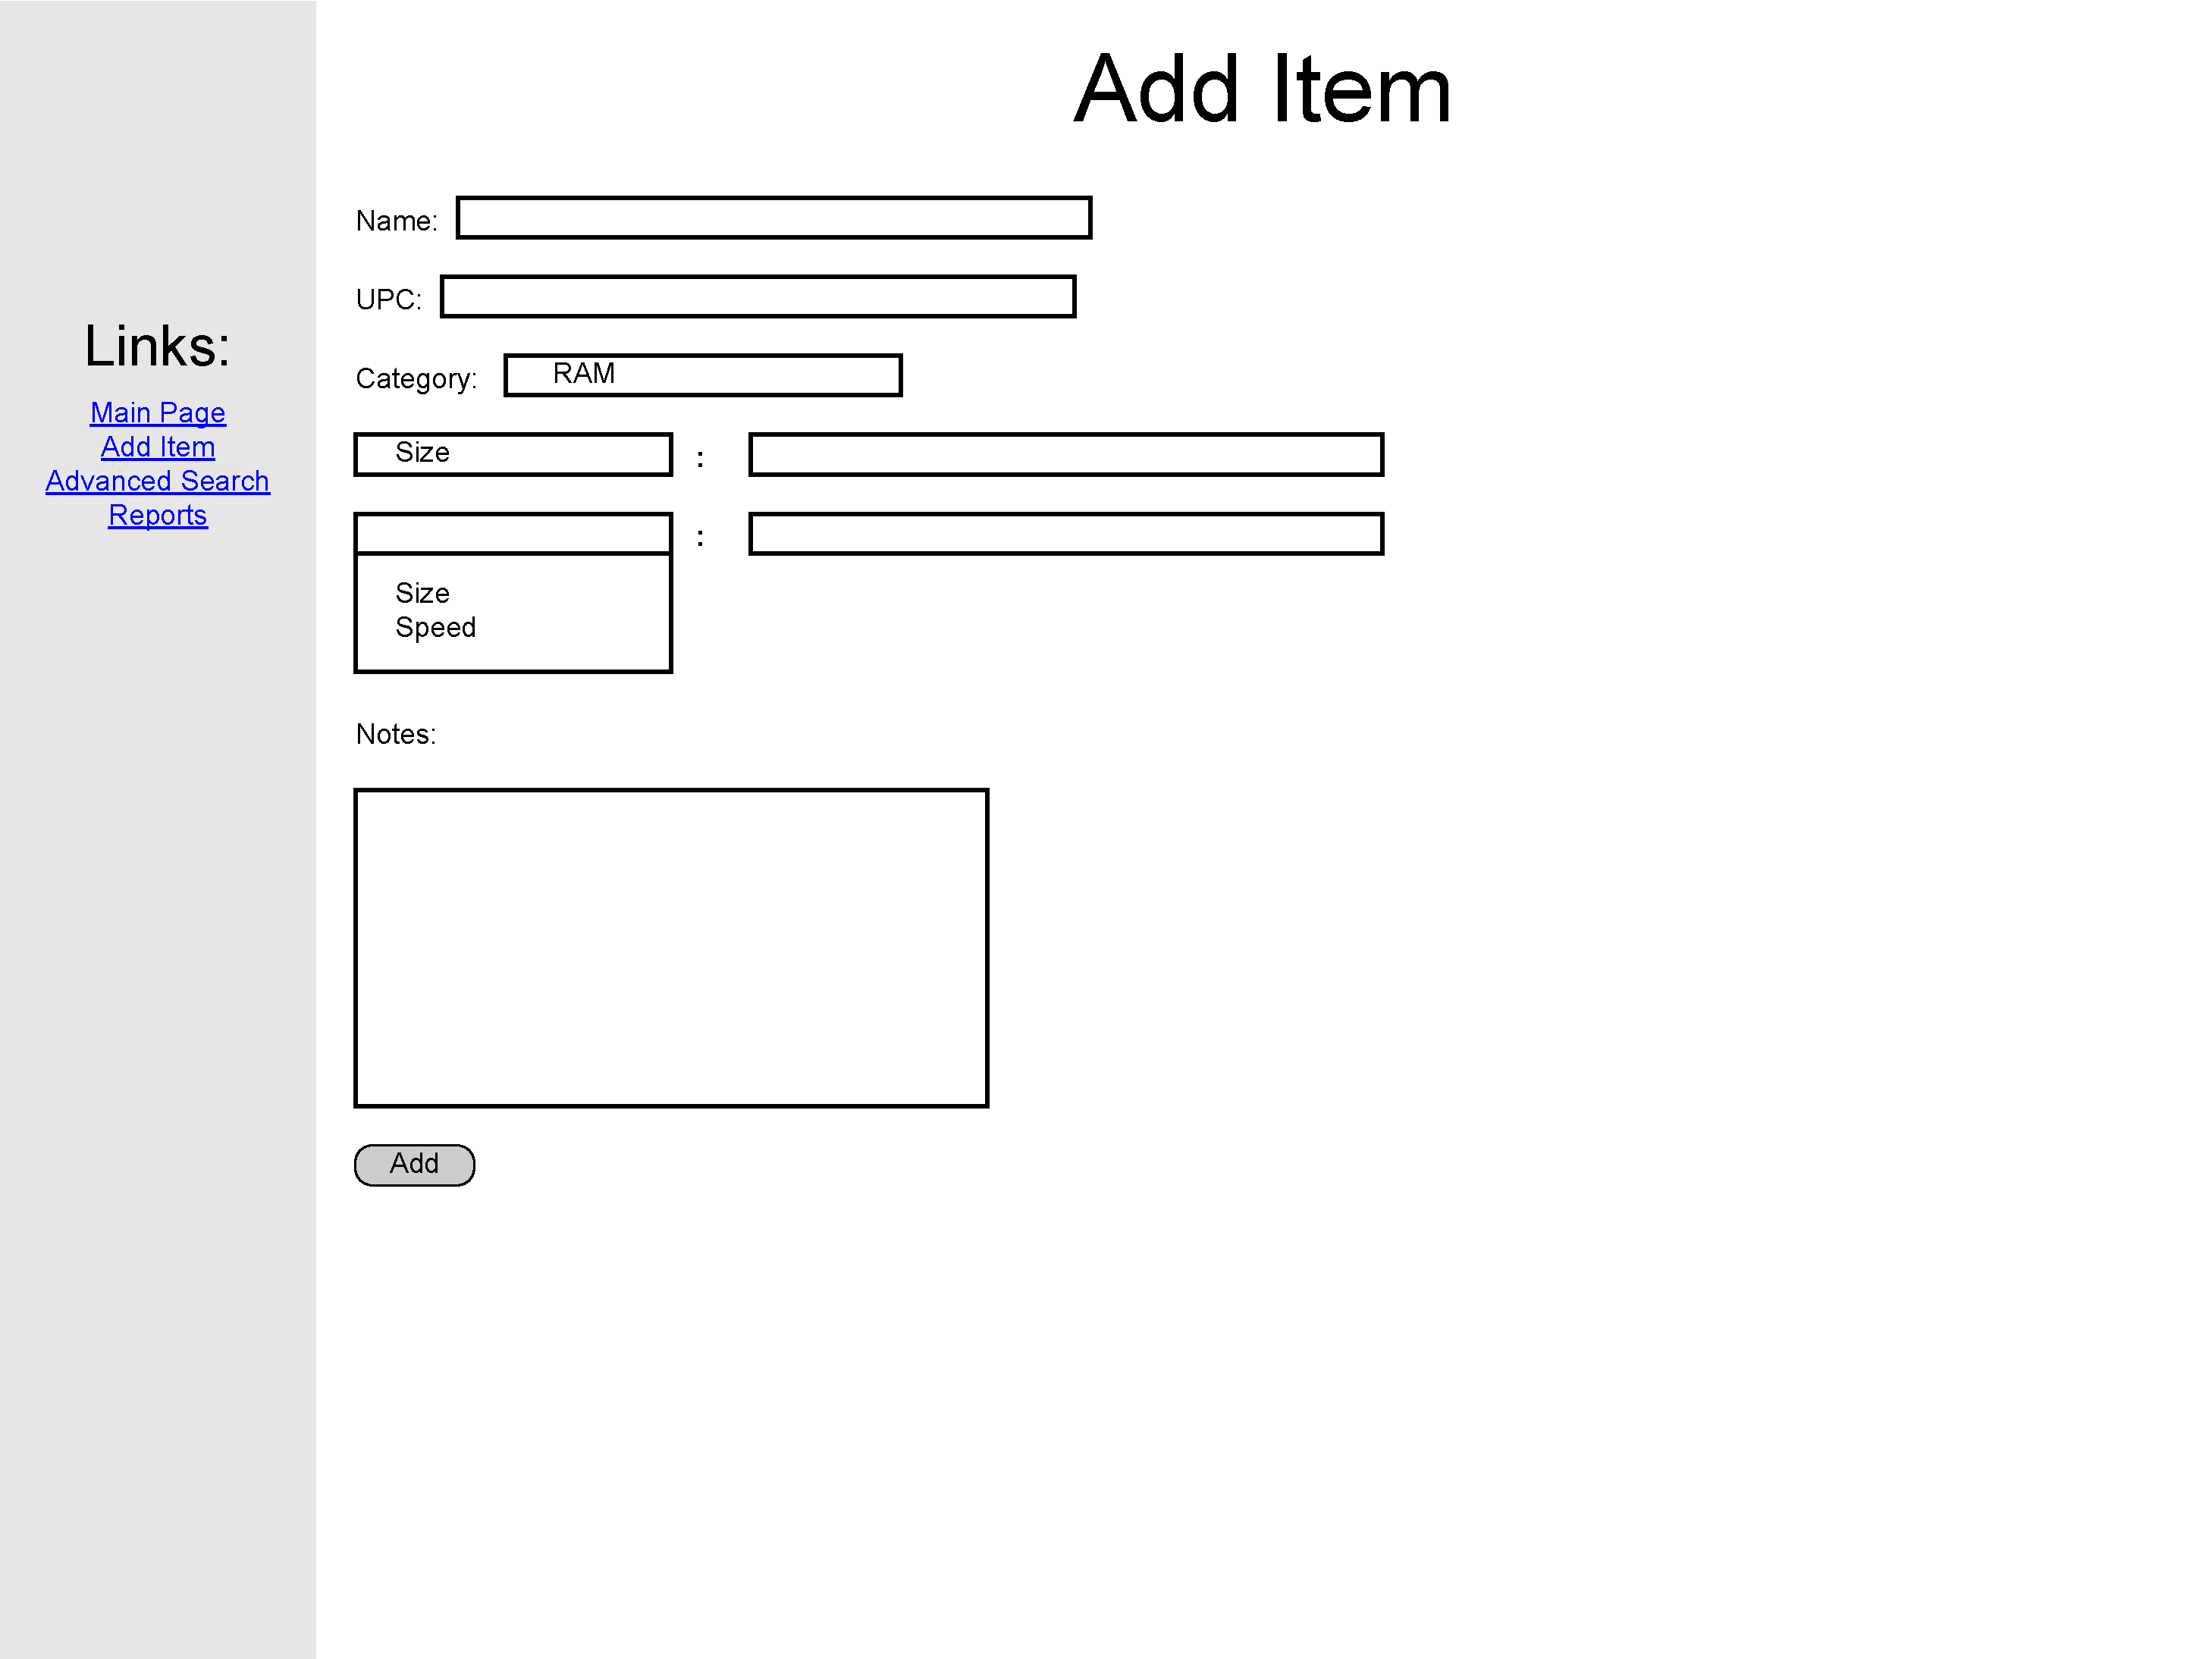
\includegraphics[keepaspectratio, width=4.5in]{addItemF0S3.pdf}\\
The add item page after one attribute key has been selected and another field added
\end{tabular}\\
~\\
~\\
\begin{tabular}{ p{4.5in} }
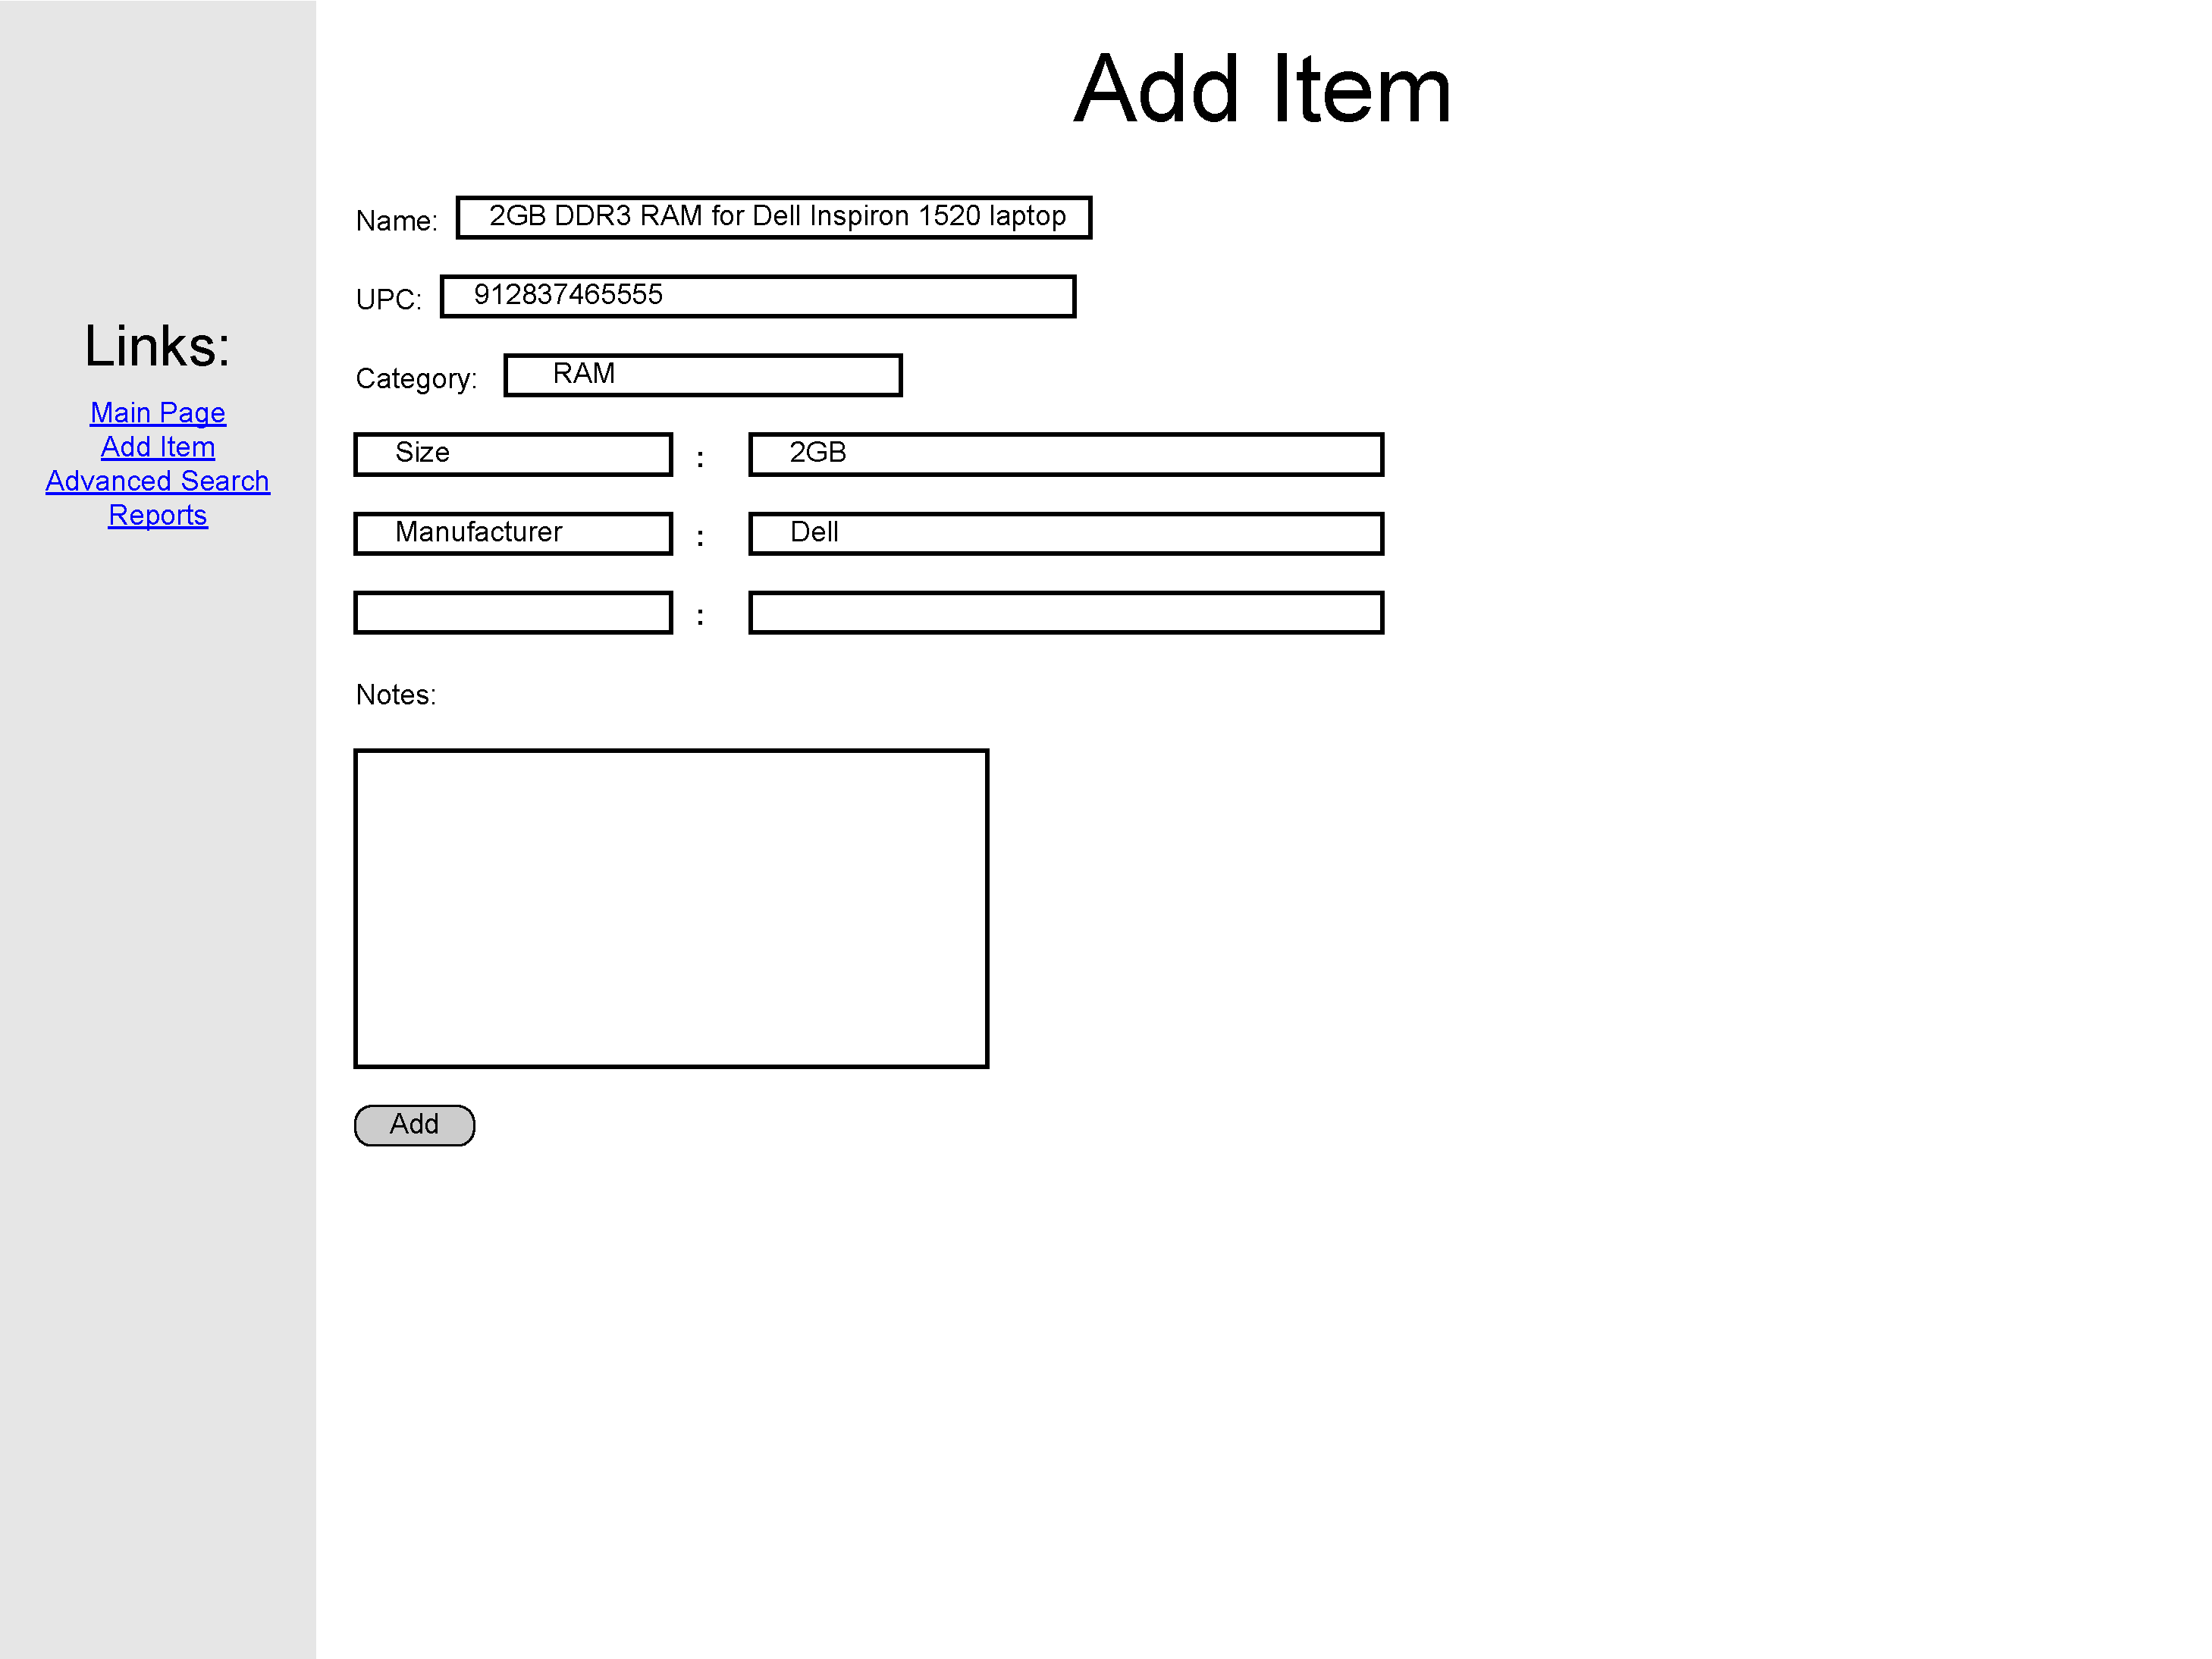
\includegraphics[keepaspectratio, width=4.5in]{addItemF0S5.pdf}\\
The add item page with data filled in
\end{tabular}\\
~\\
~\\
\begin{tabular}{ p{4.5in} }
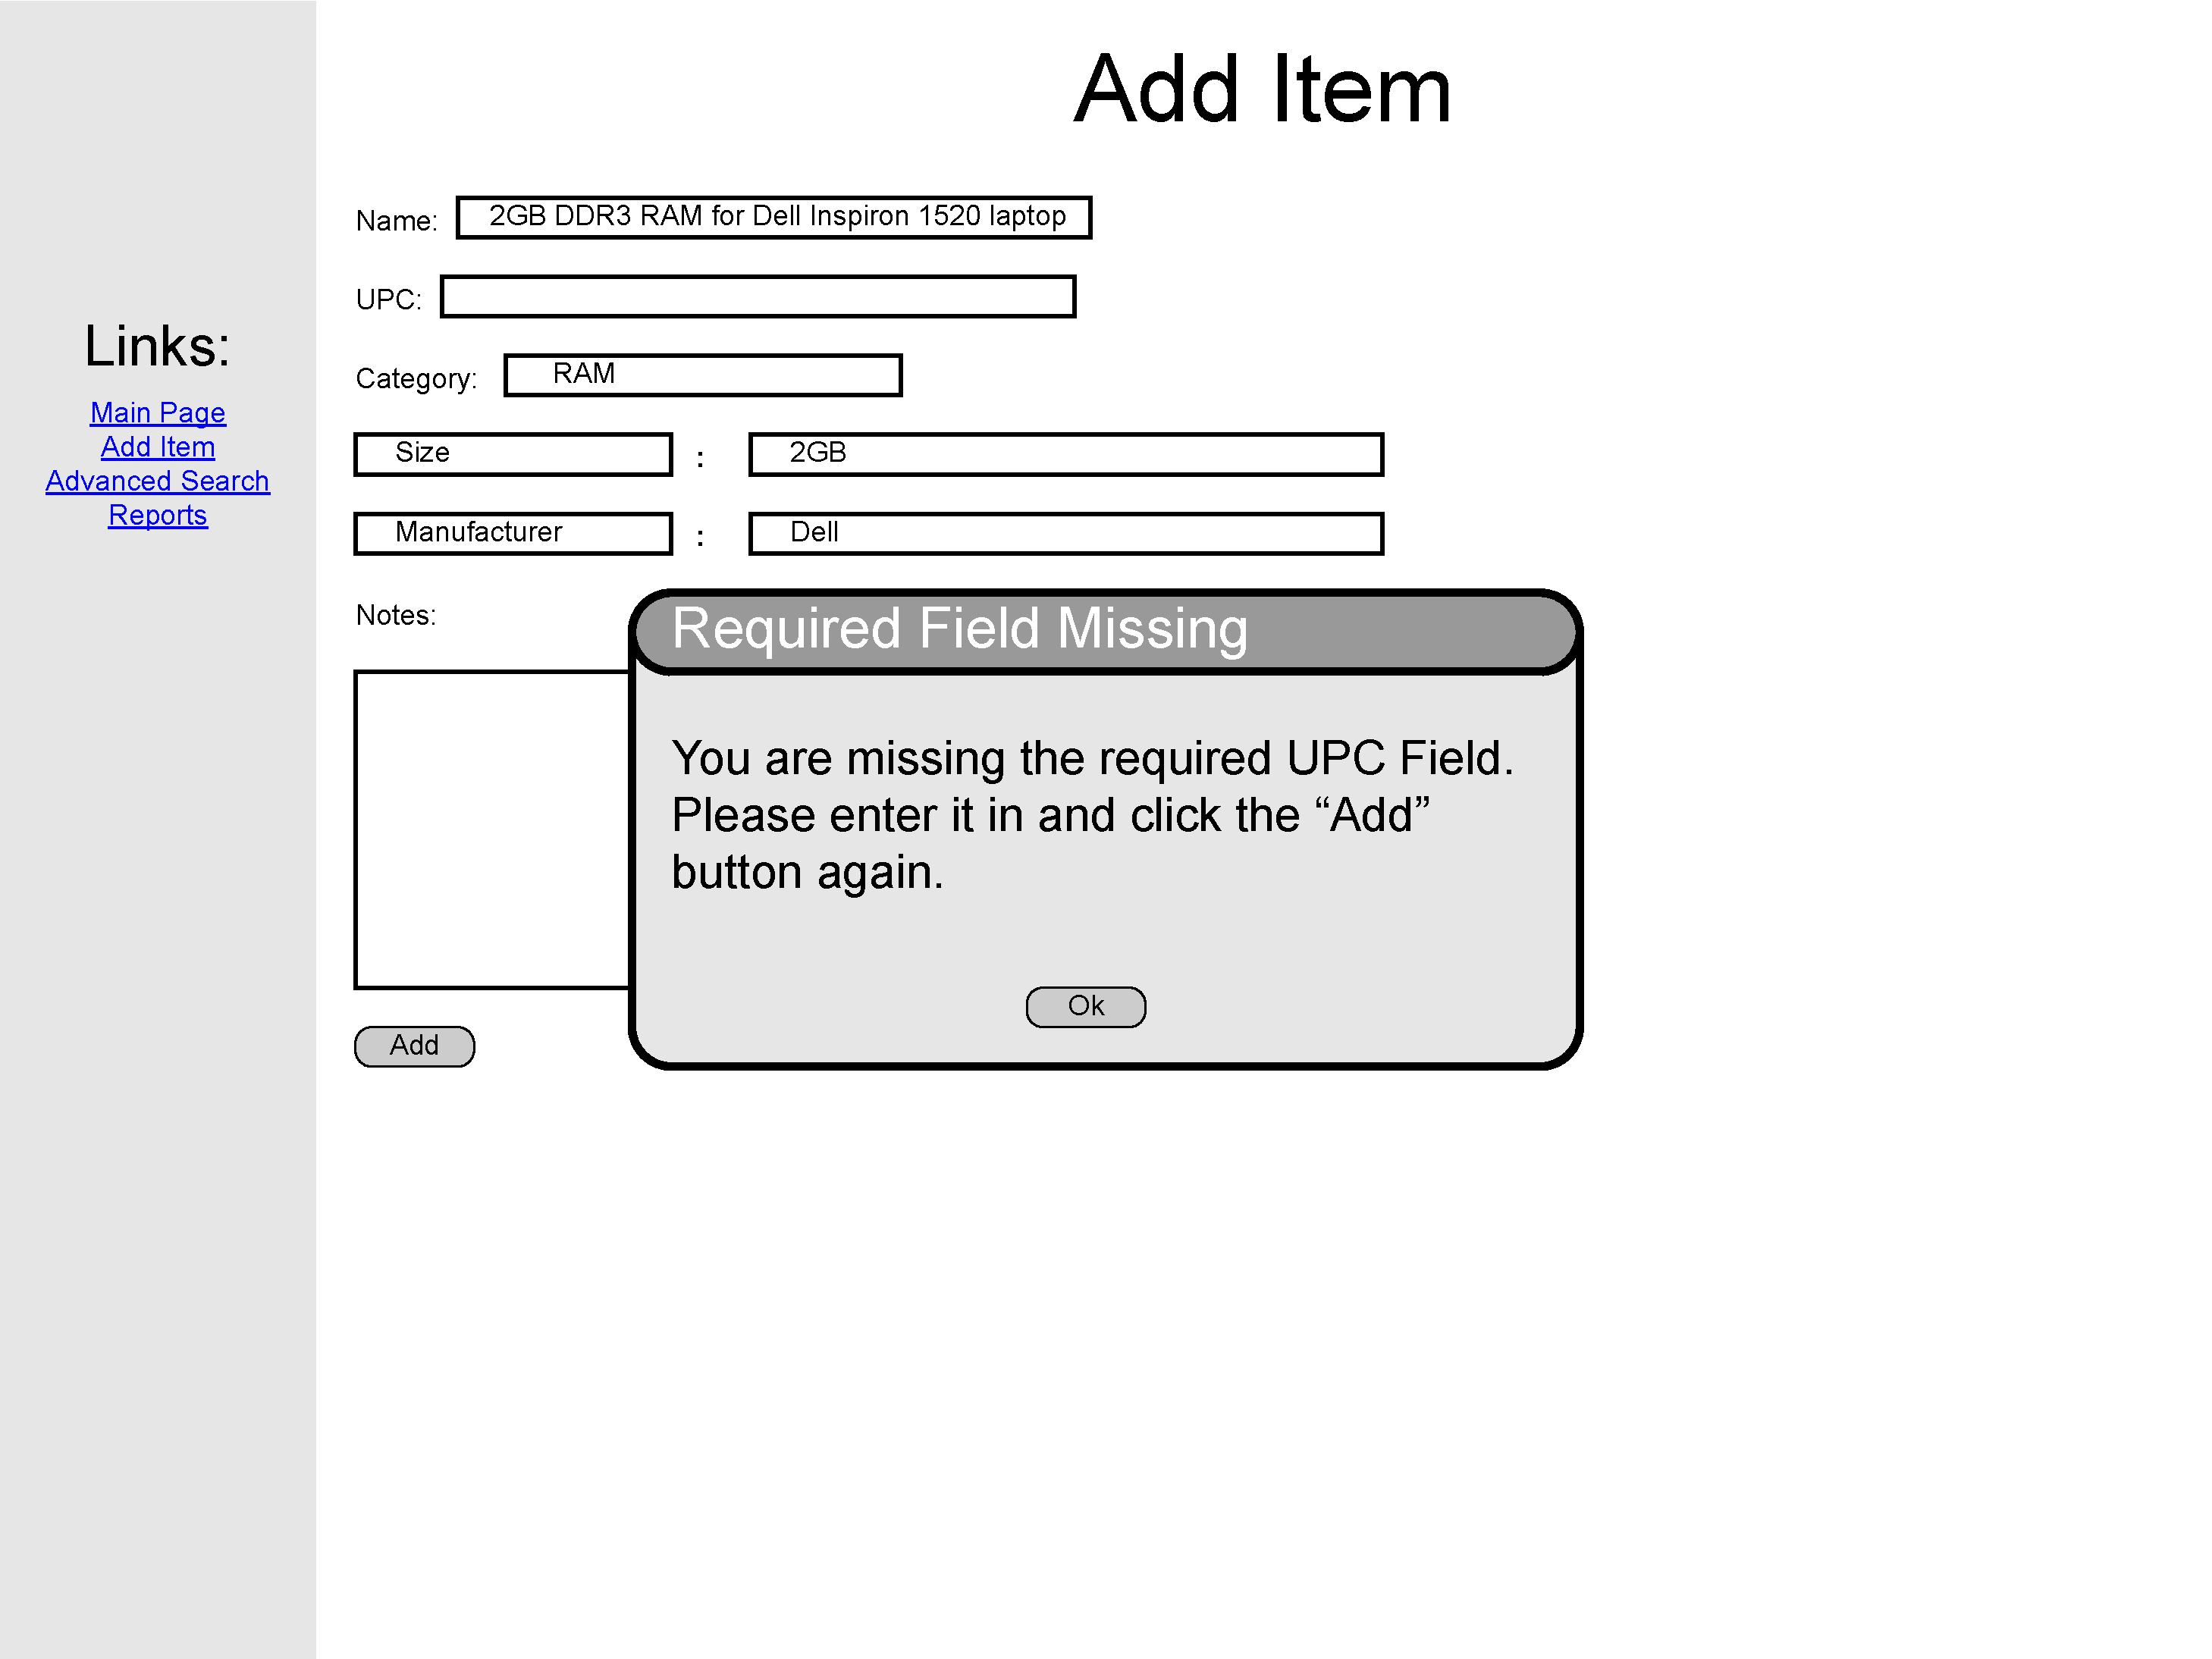
\includegraphics[keepaspectratio, width=4.5in]{addItemF1S5.pdf} \\
Popup message informing the user that the required UPC field is missing
\end{tabular}\\
~\\
~\\
\begin{tabular}{ p{4.5in} }
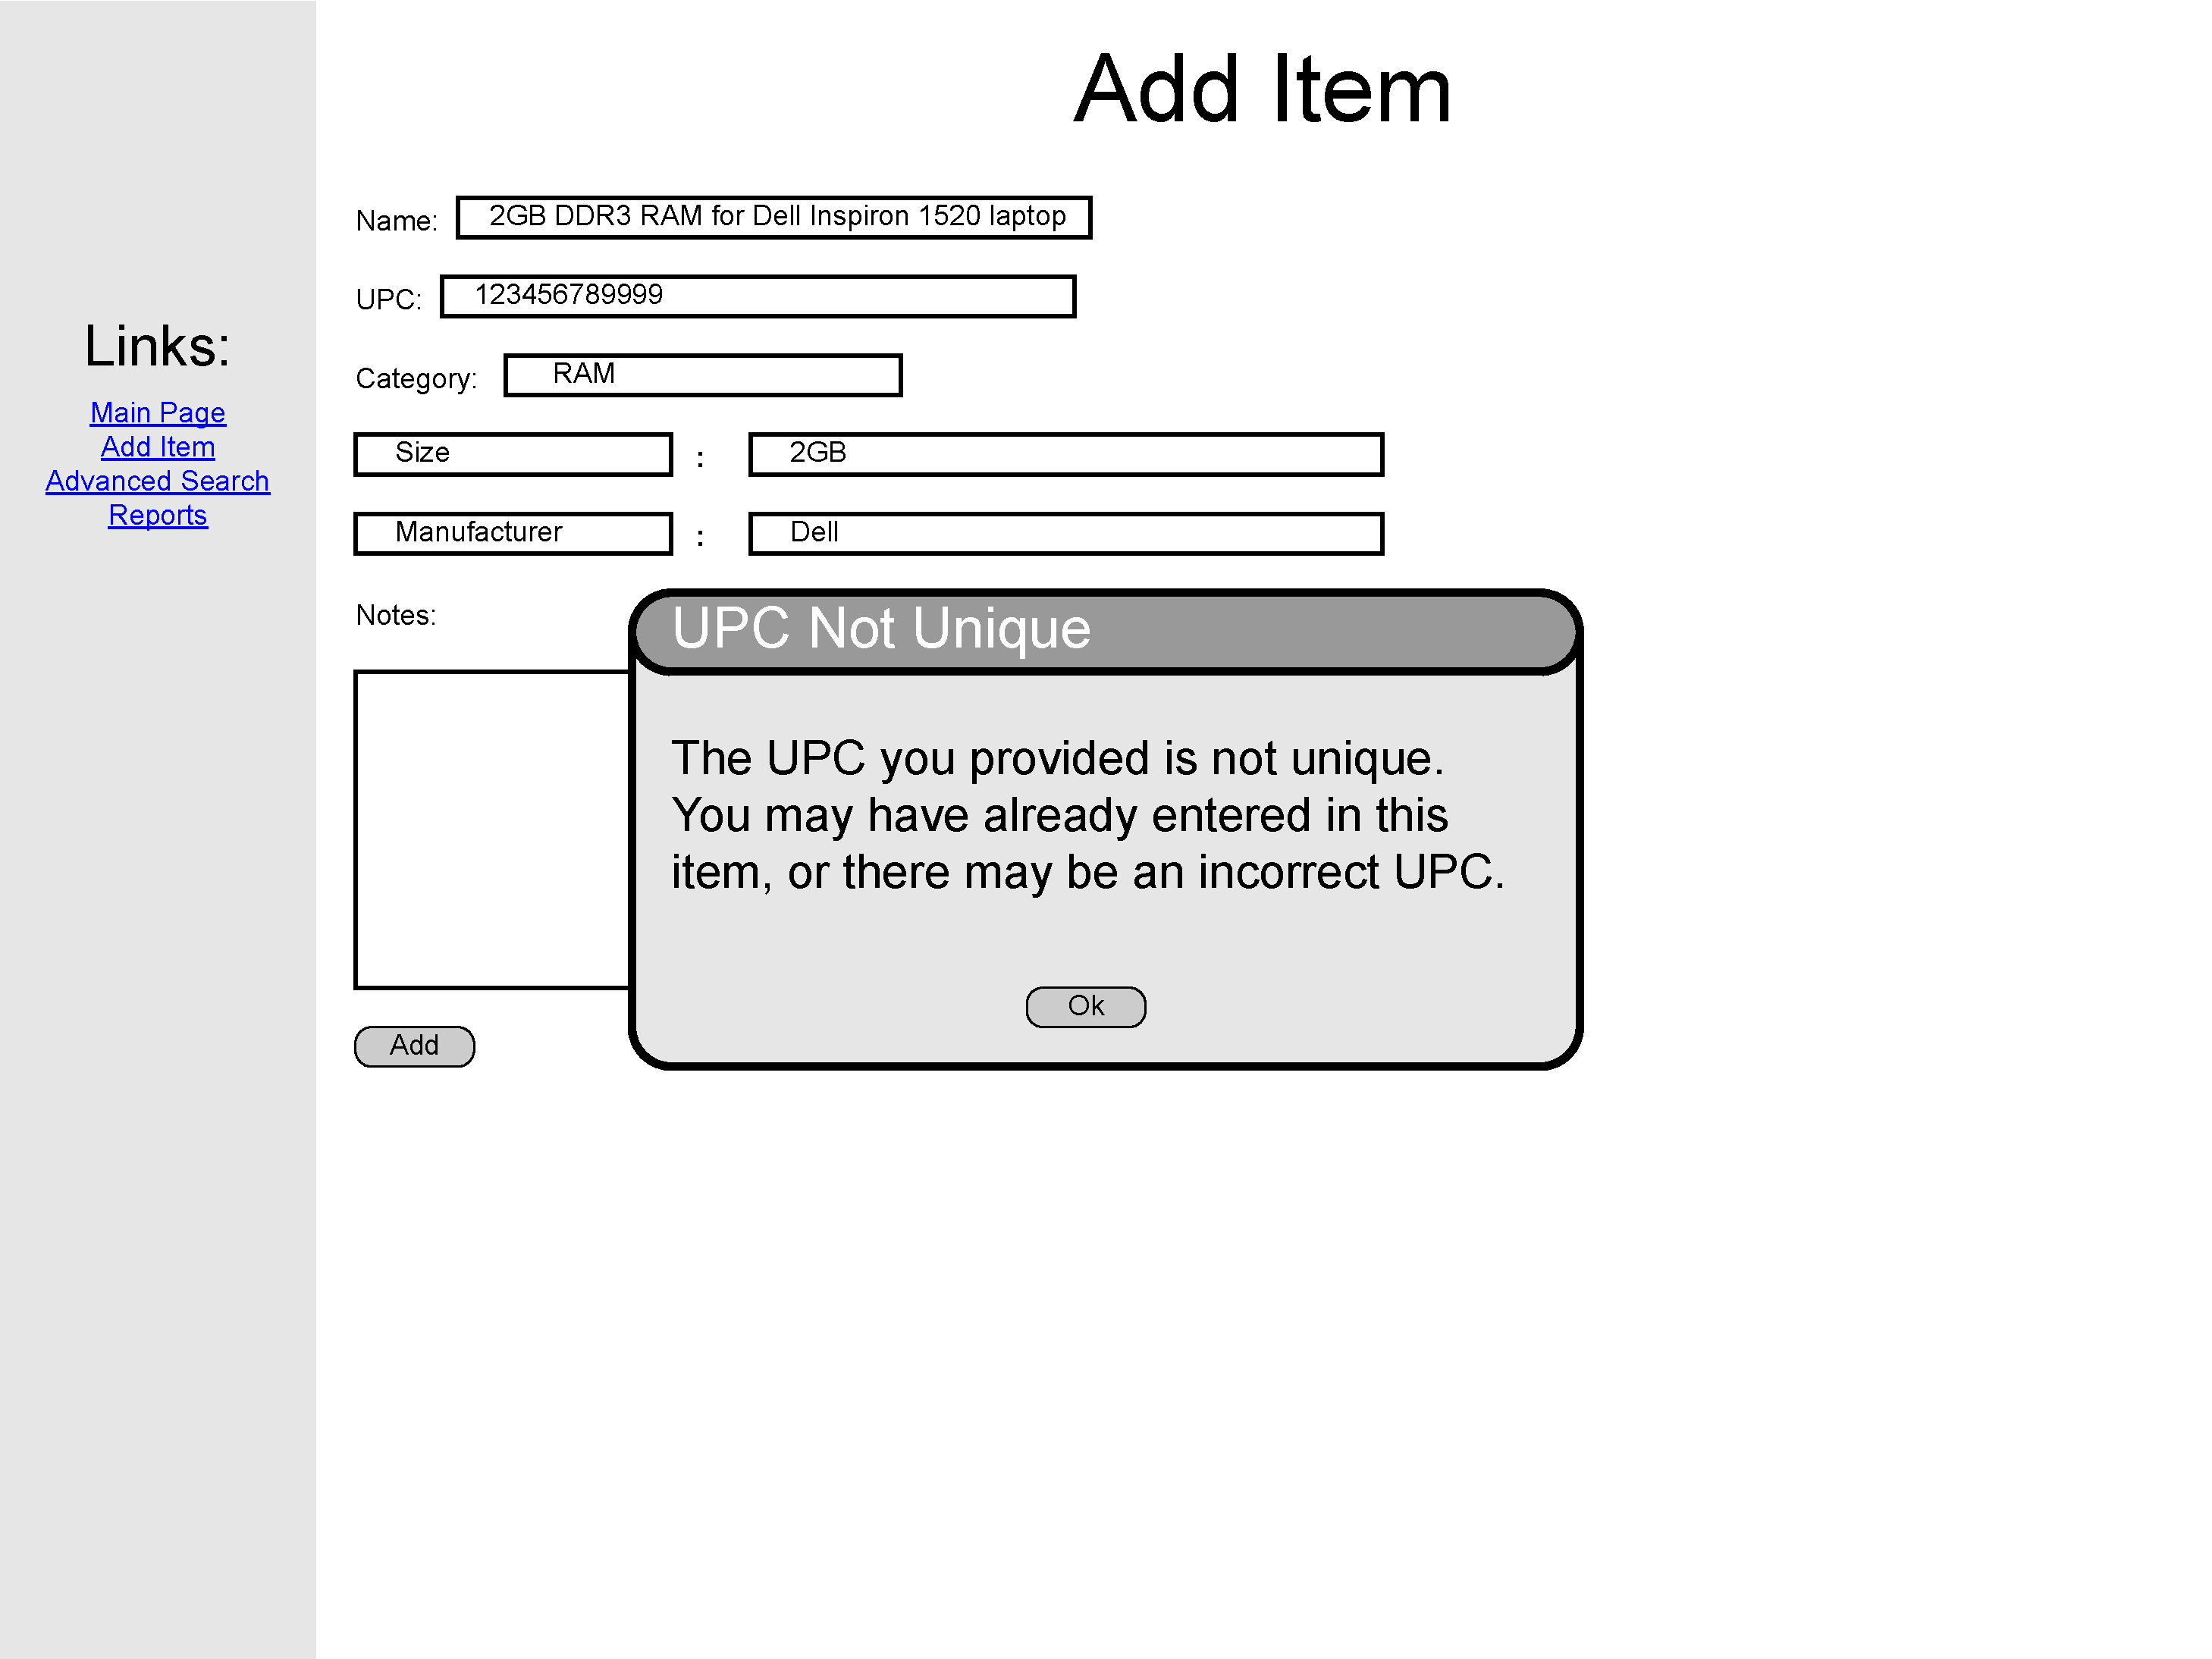
\includegraphics[keepaspectratio, width=4.5in]{addItemF2S5.pdf} \\
Popup message informing the user that the UPC entered has been previously entered
\end{tabular}\\
~\\
~\\
\begin{tabular}{ p{4.5in} }
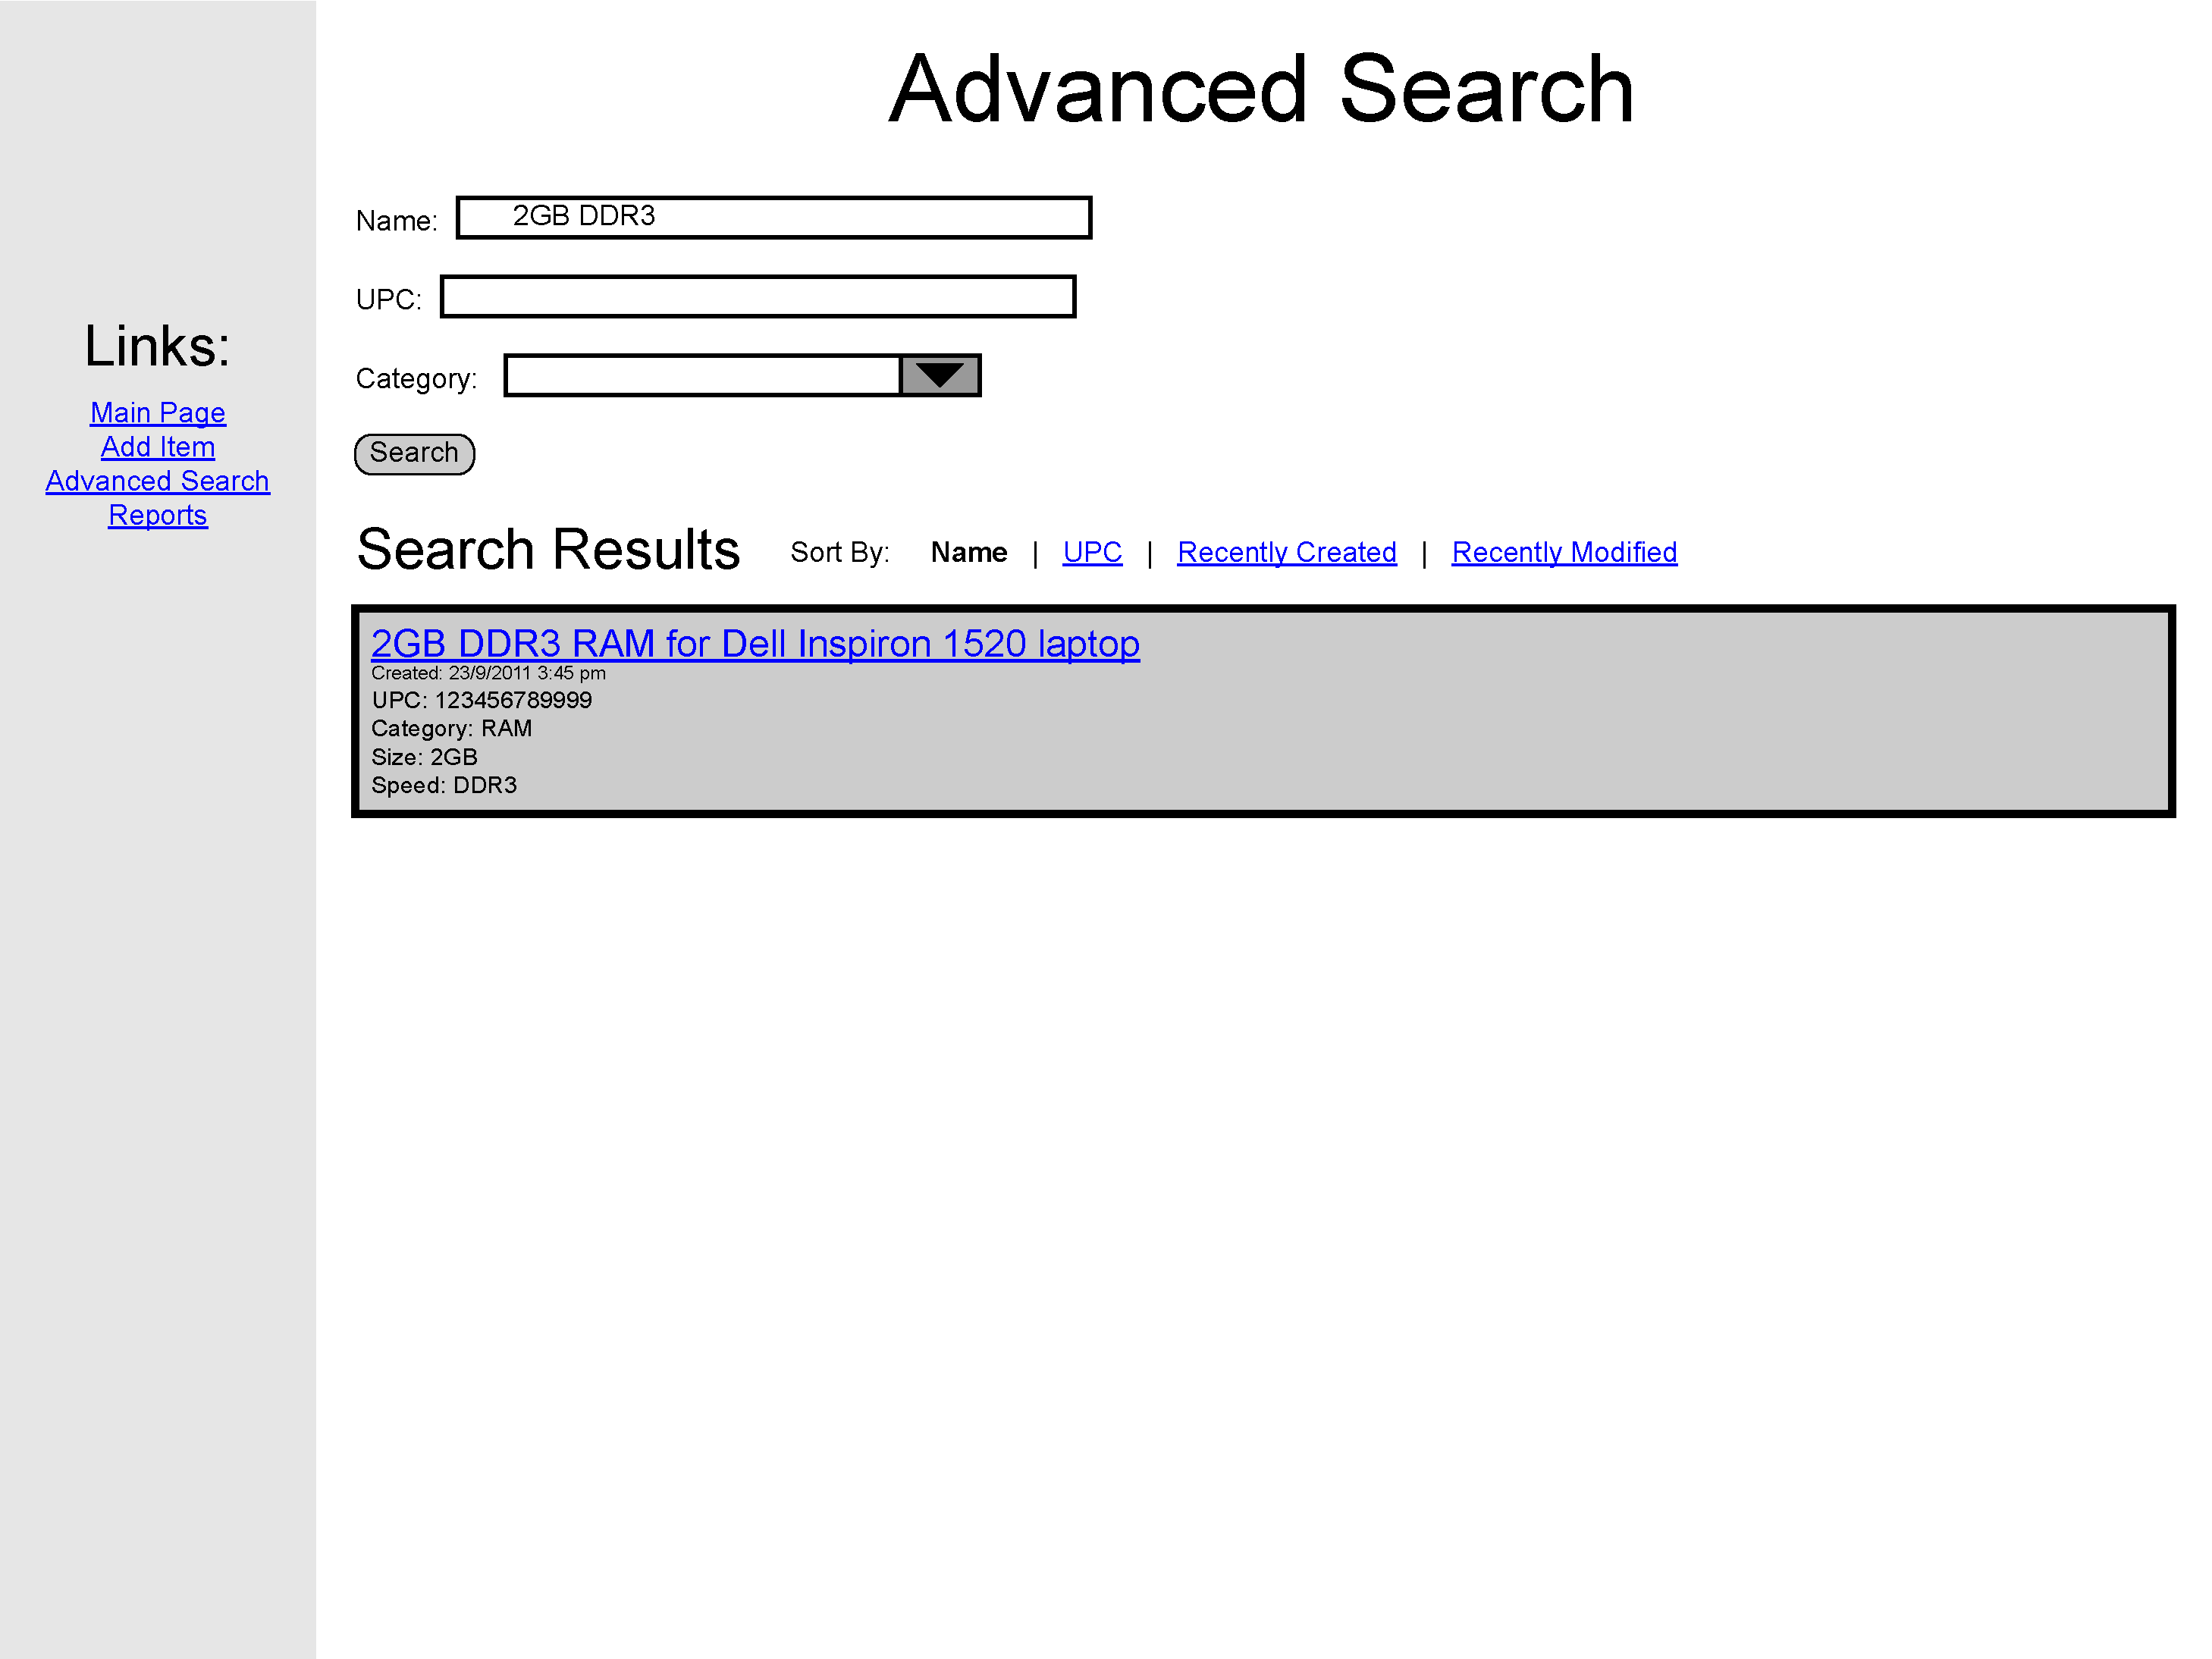
\includegraphics[keepaspectratio, width=4.5in]{basicSearchF0S1.pdf} \\
The results of the basic search
\end{tabular}\\
~\\
~\\
\begin{tabular}{ p{4.5in} }
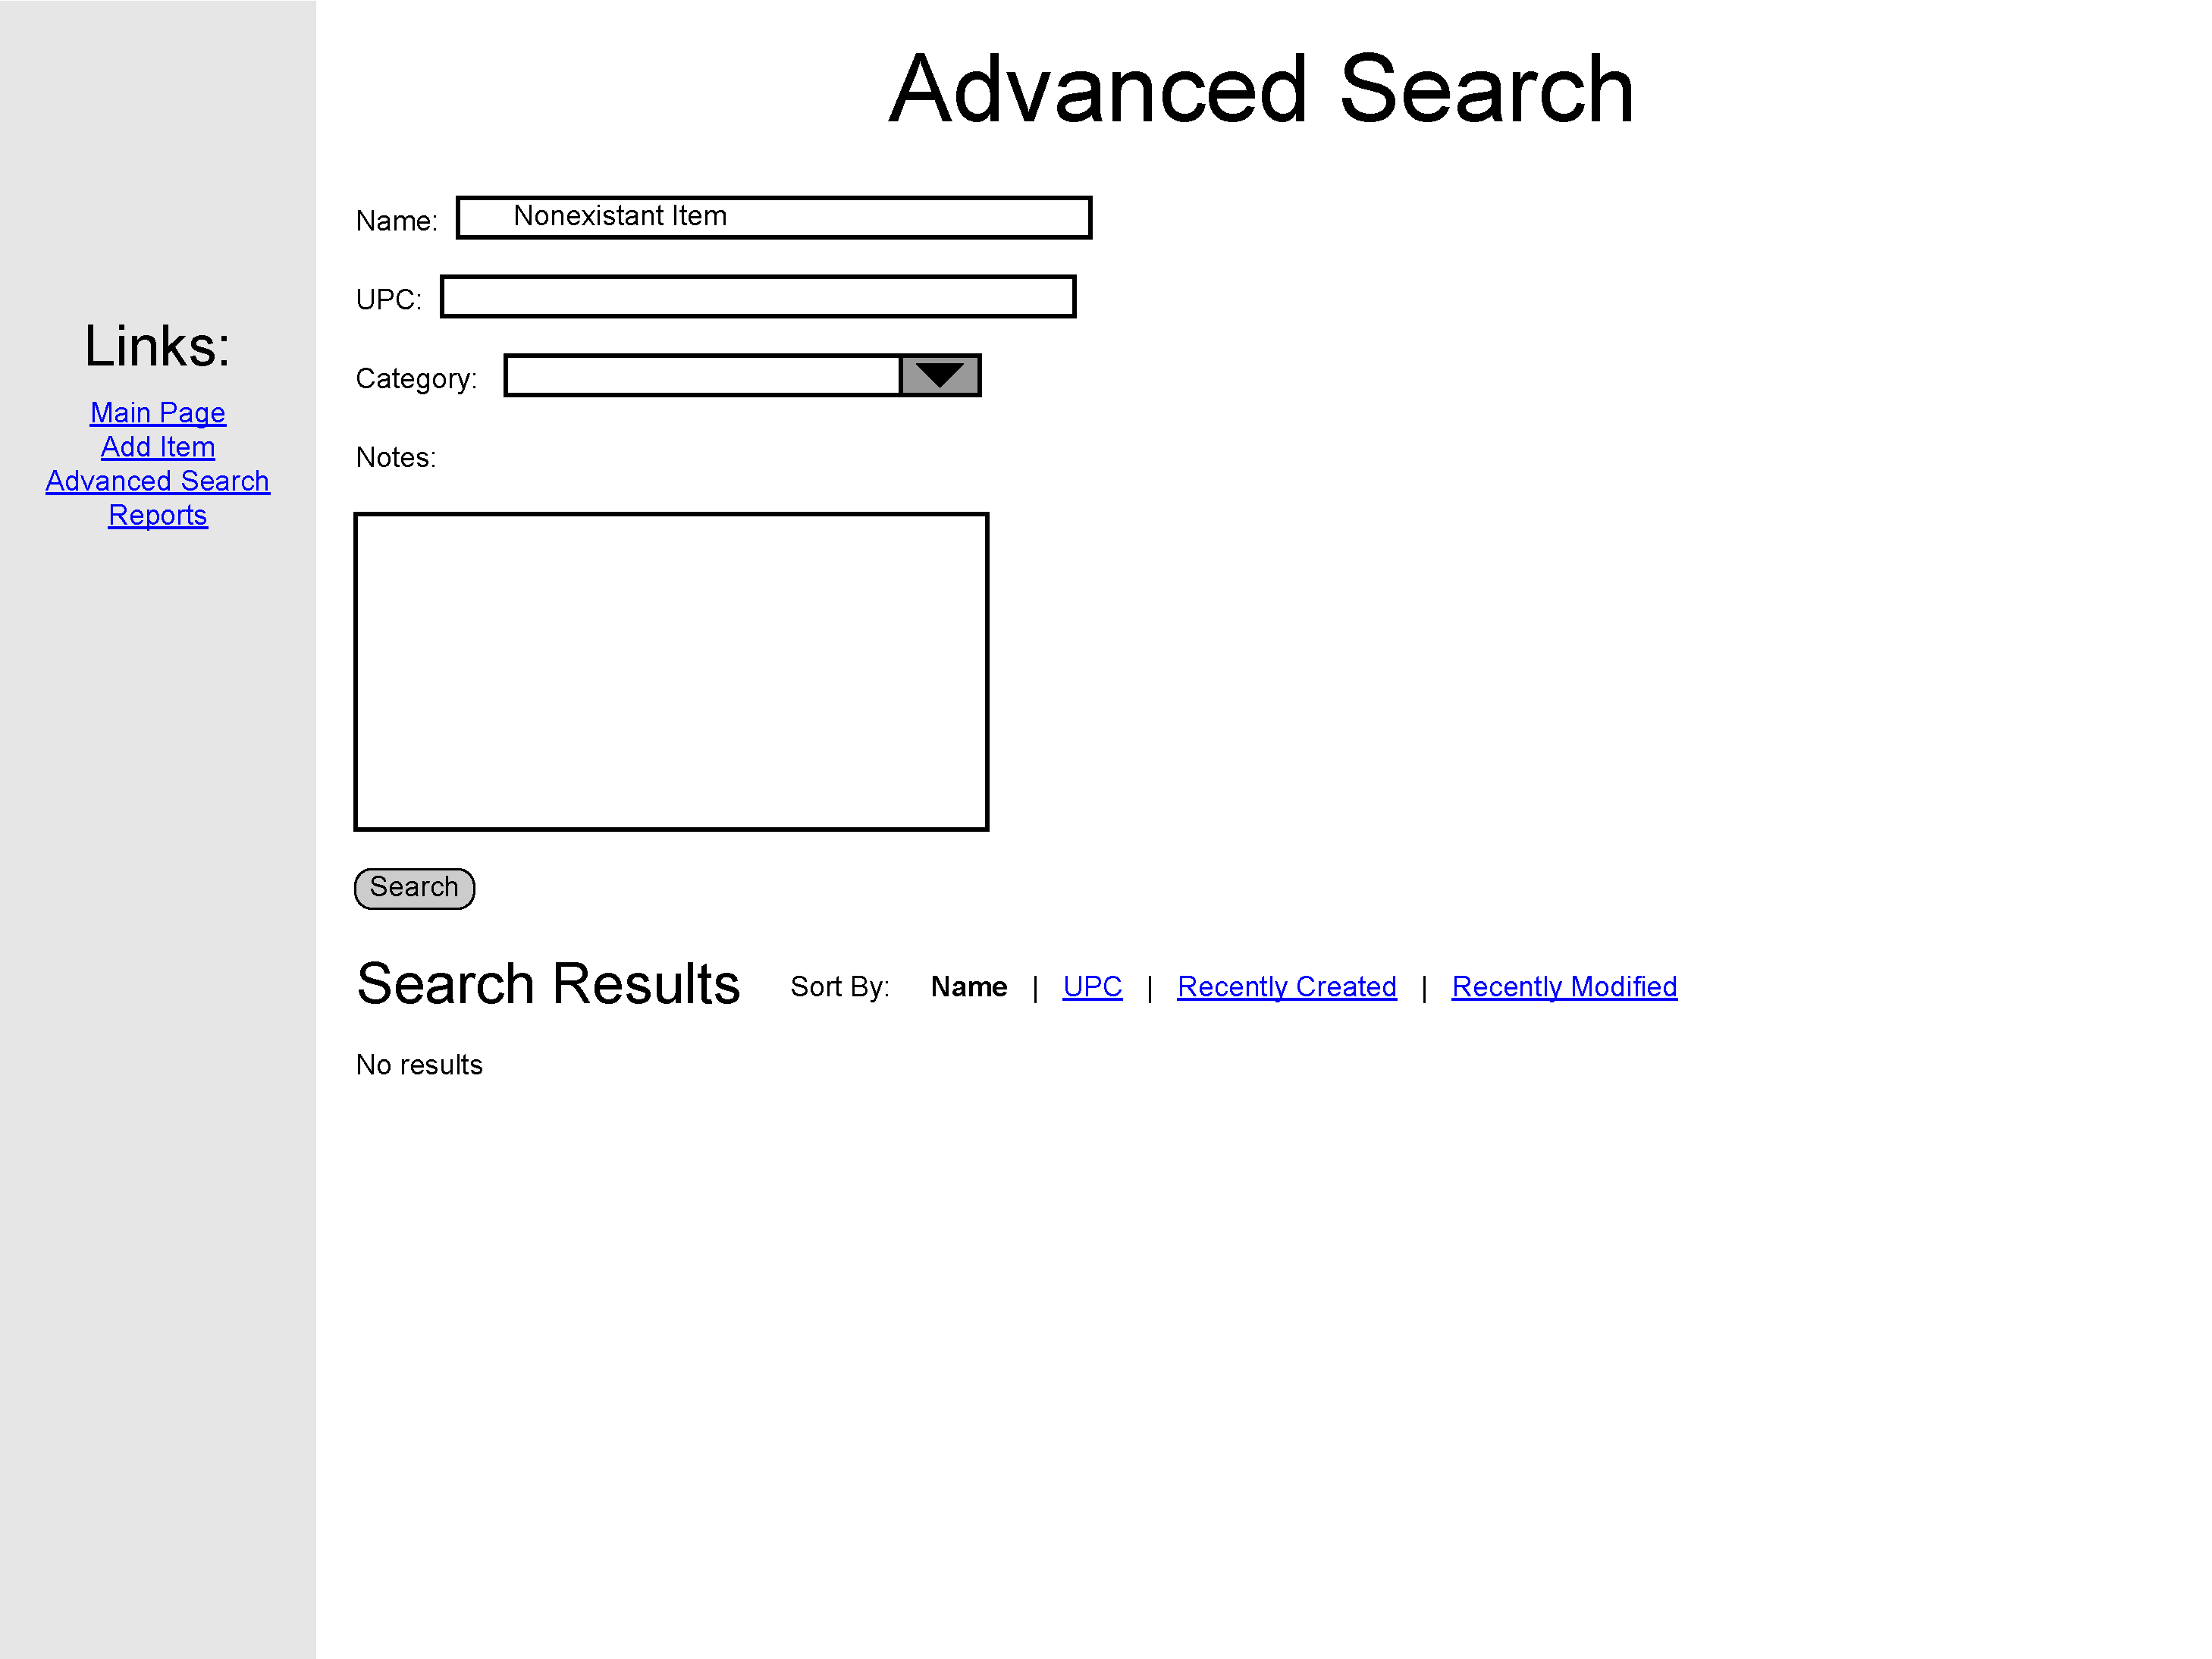
\includegraphics[keepaspectratio, width=4.5in]{basicSearchF2S1.pdf} \\
The results of the basic search when there are no matching entries
\end{tabular}\\
~\\
~\\
\begin{tabular}{ p{4.5in} }
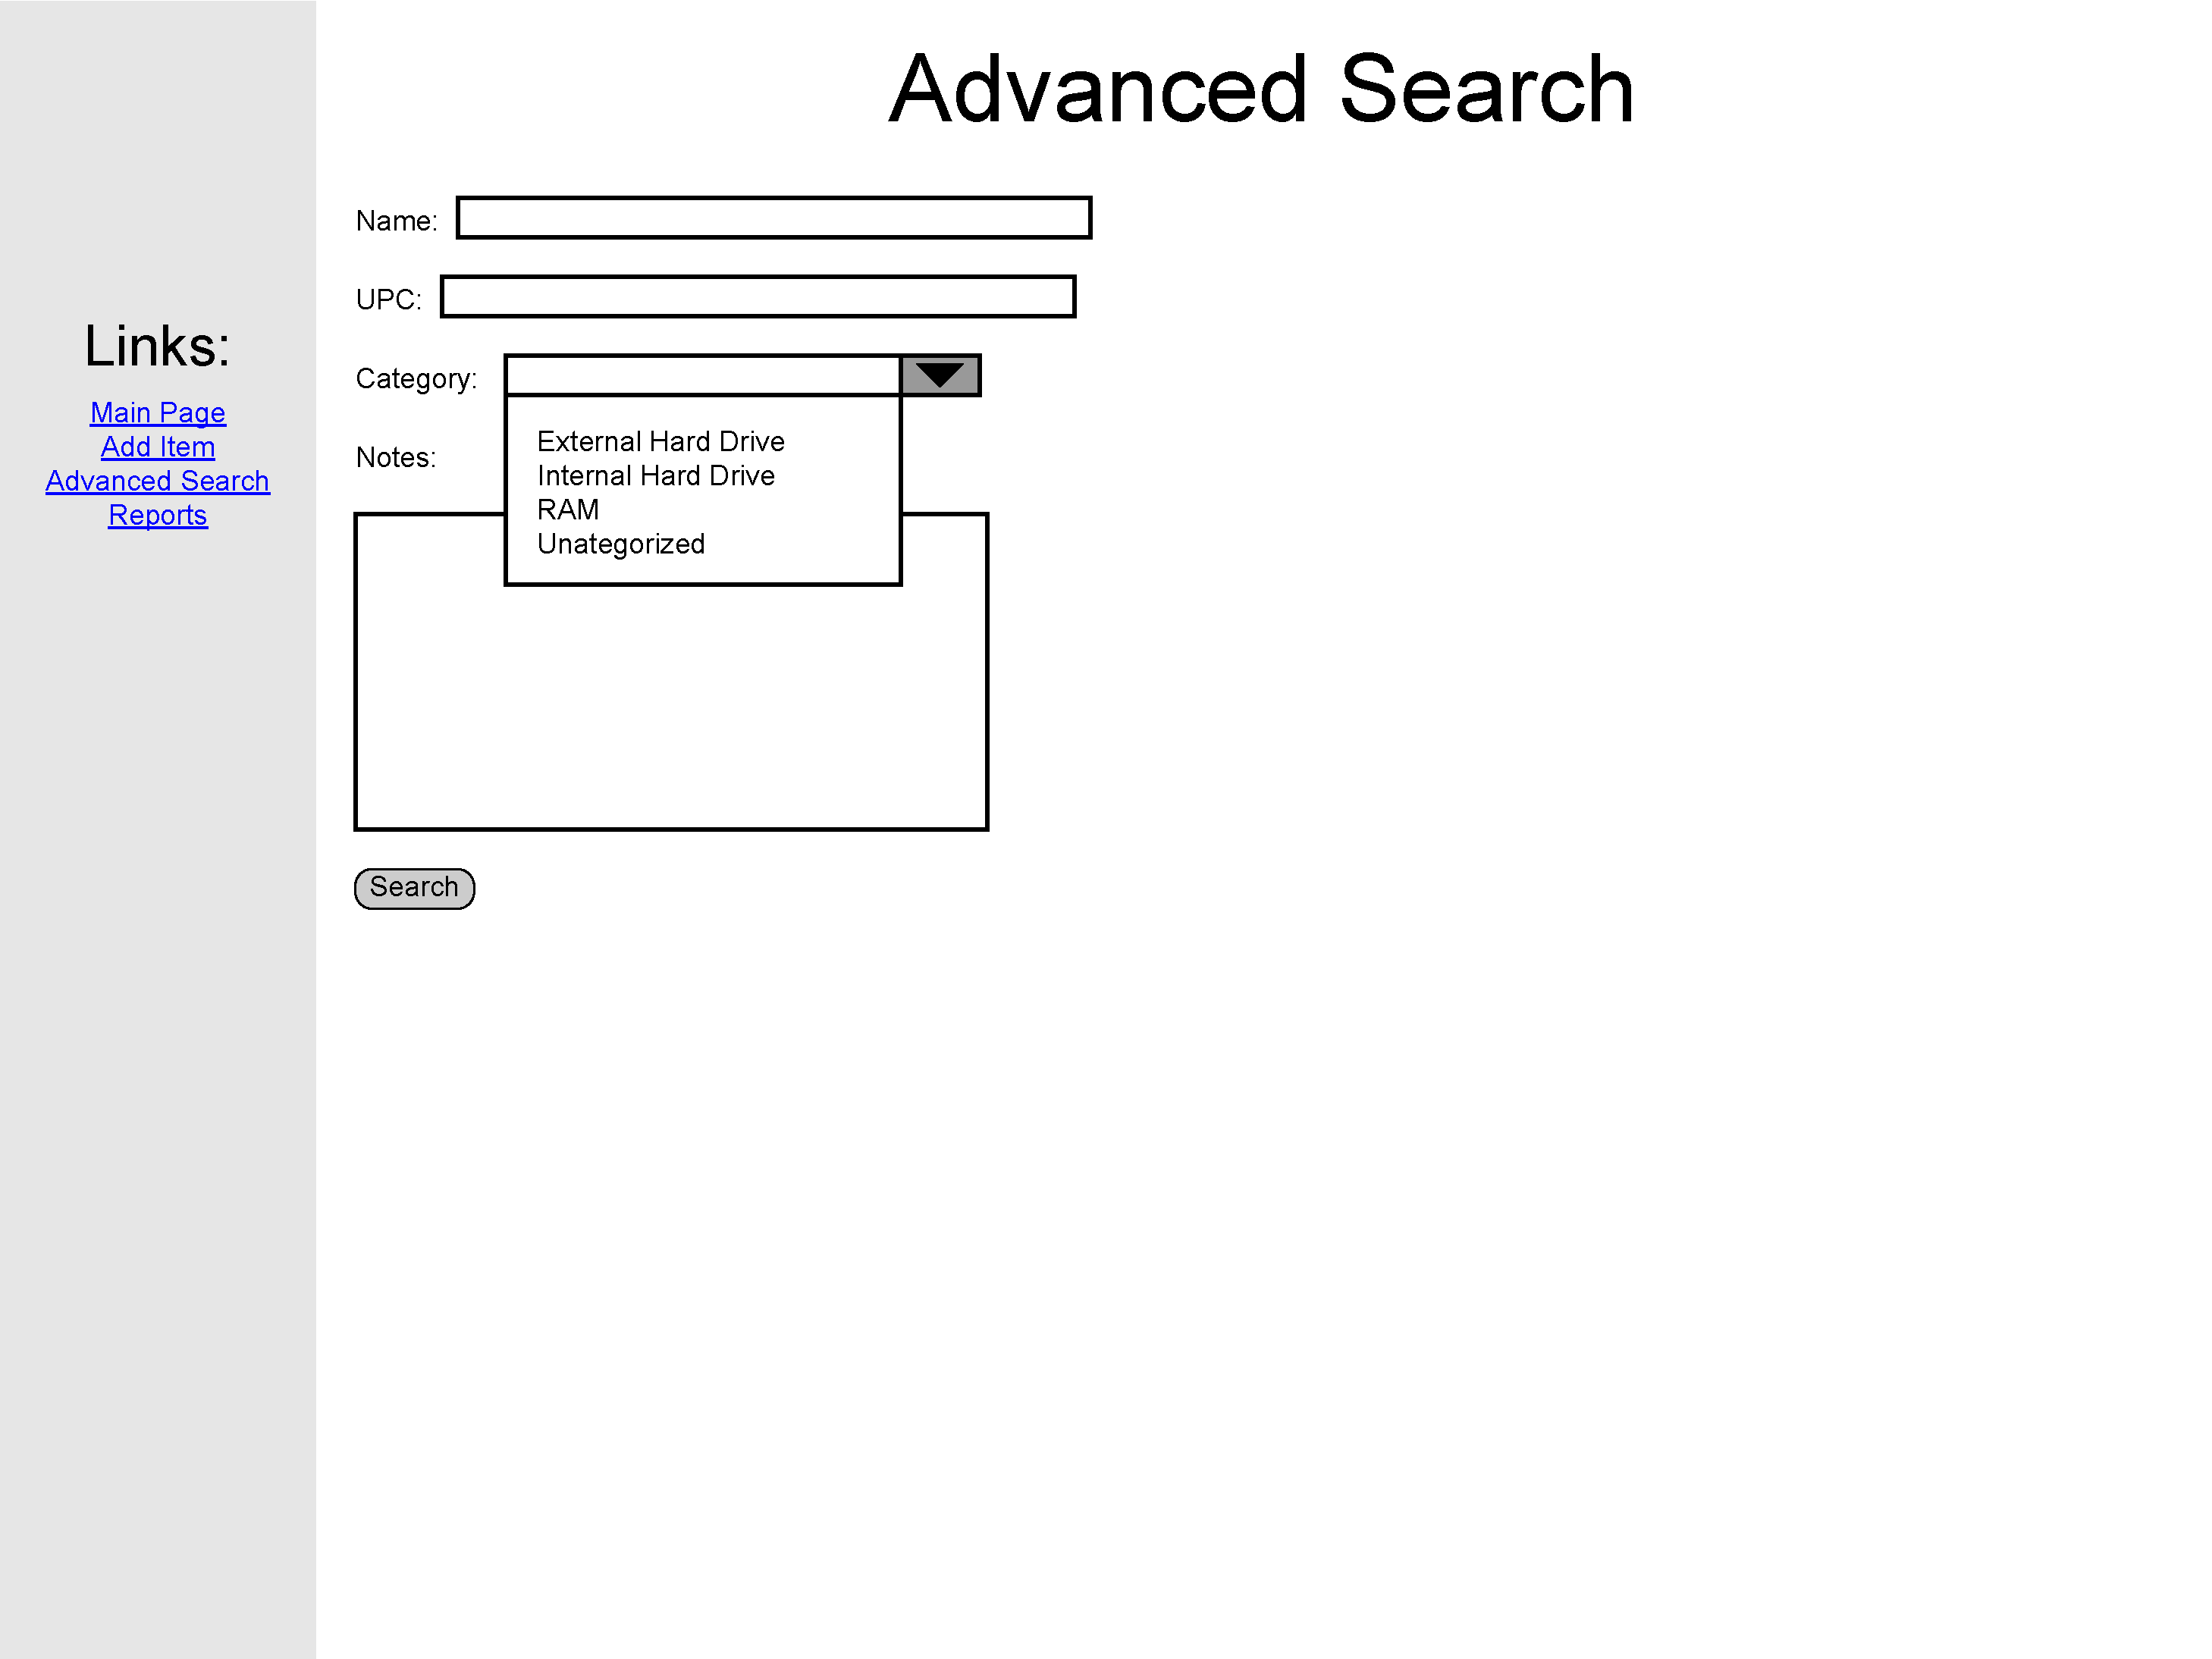
\includegraphics[keepaspectratio, width=4.5in]{advancedSearchF0S1.pdf} \\
The advanced search page with the category dropdown expanded
\end{tabular}\\
~\\
~\\
\begin{tabular}{ p{4.5in} }
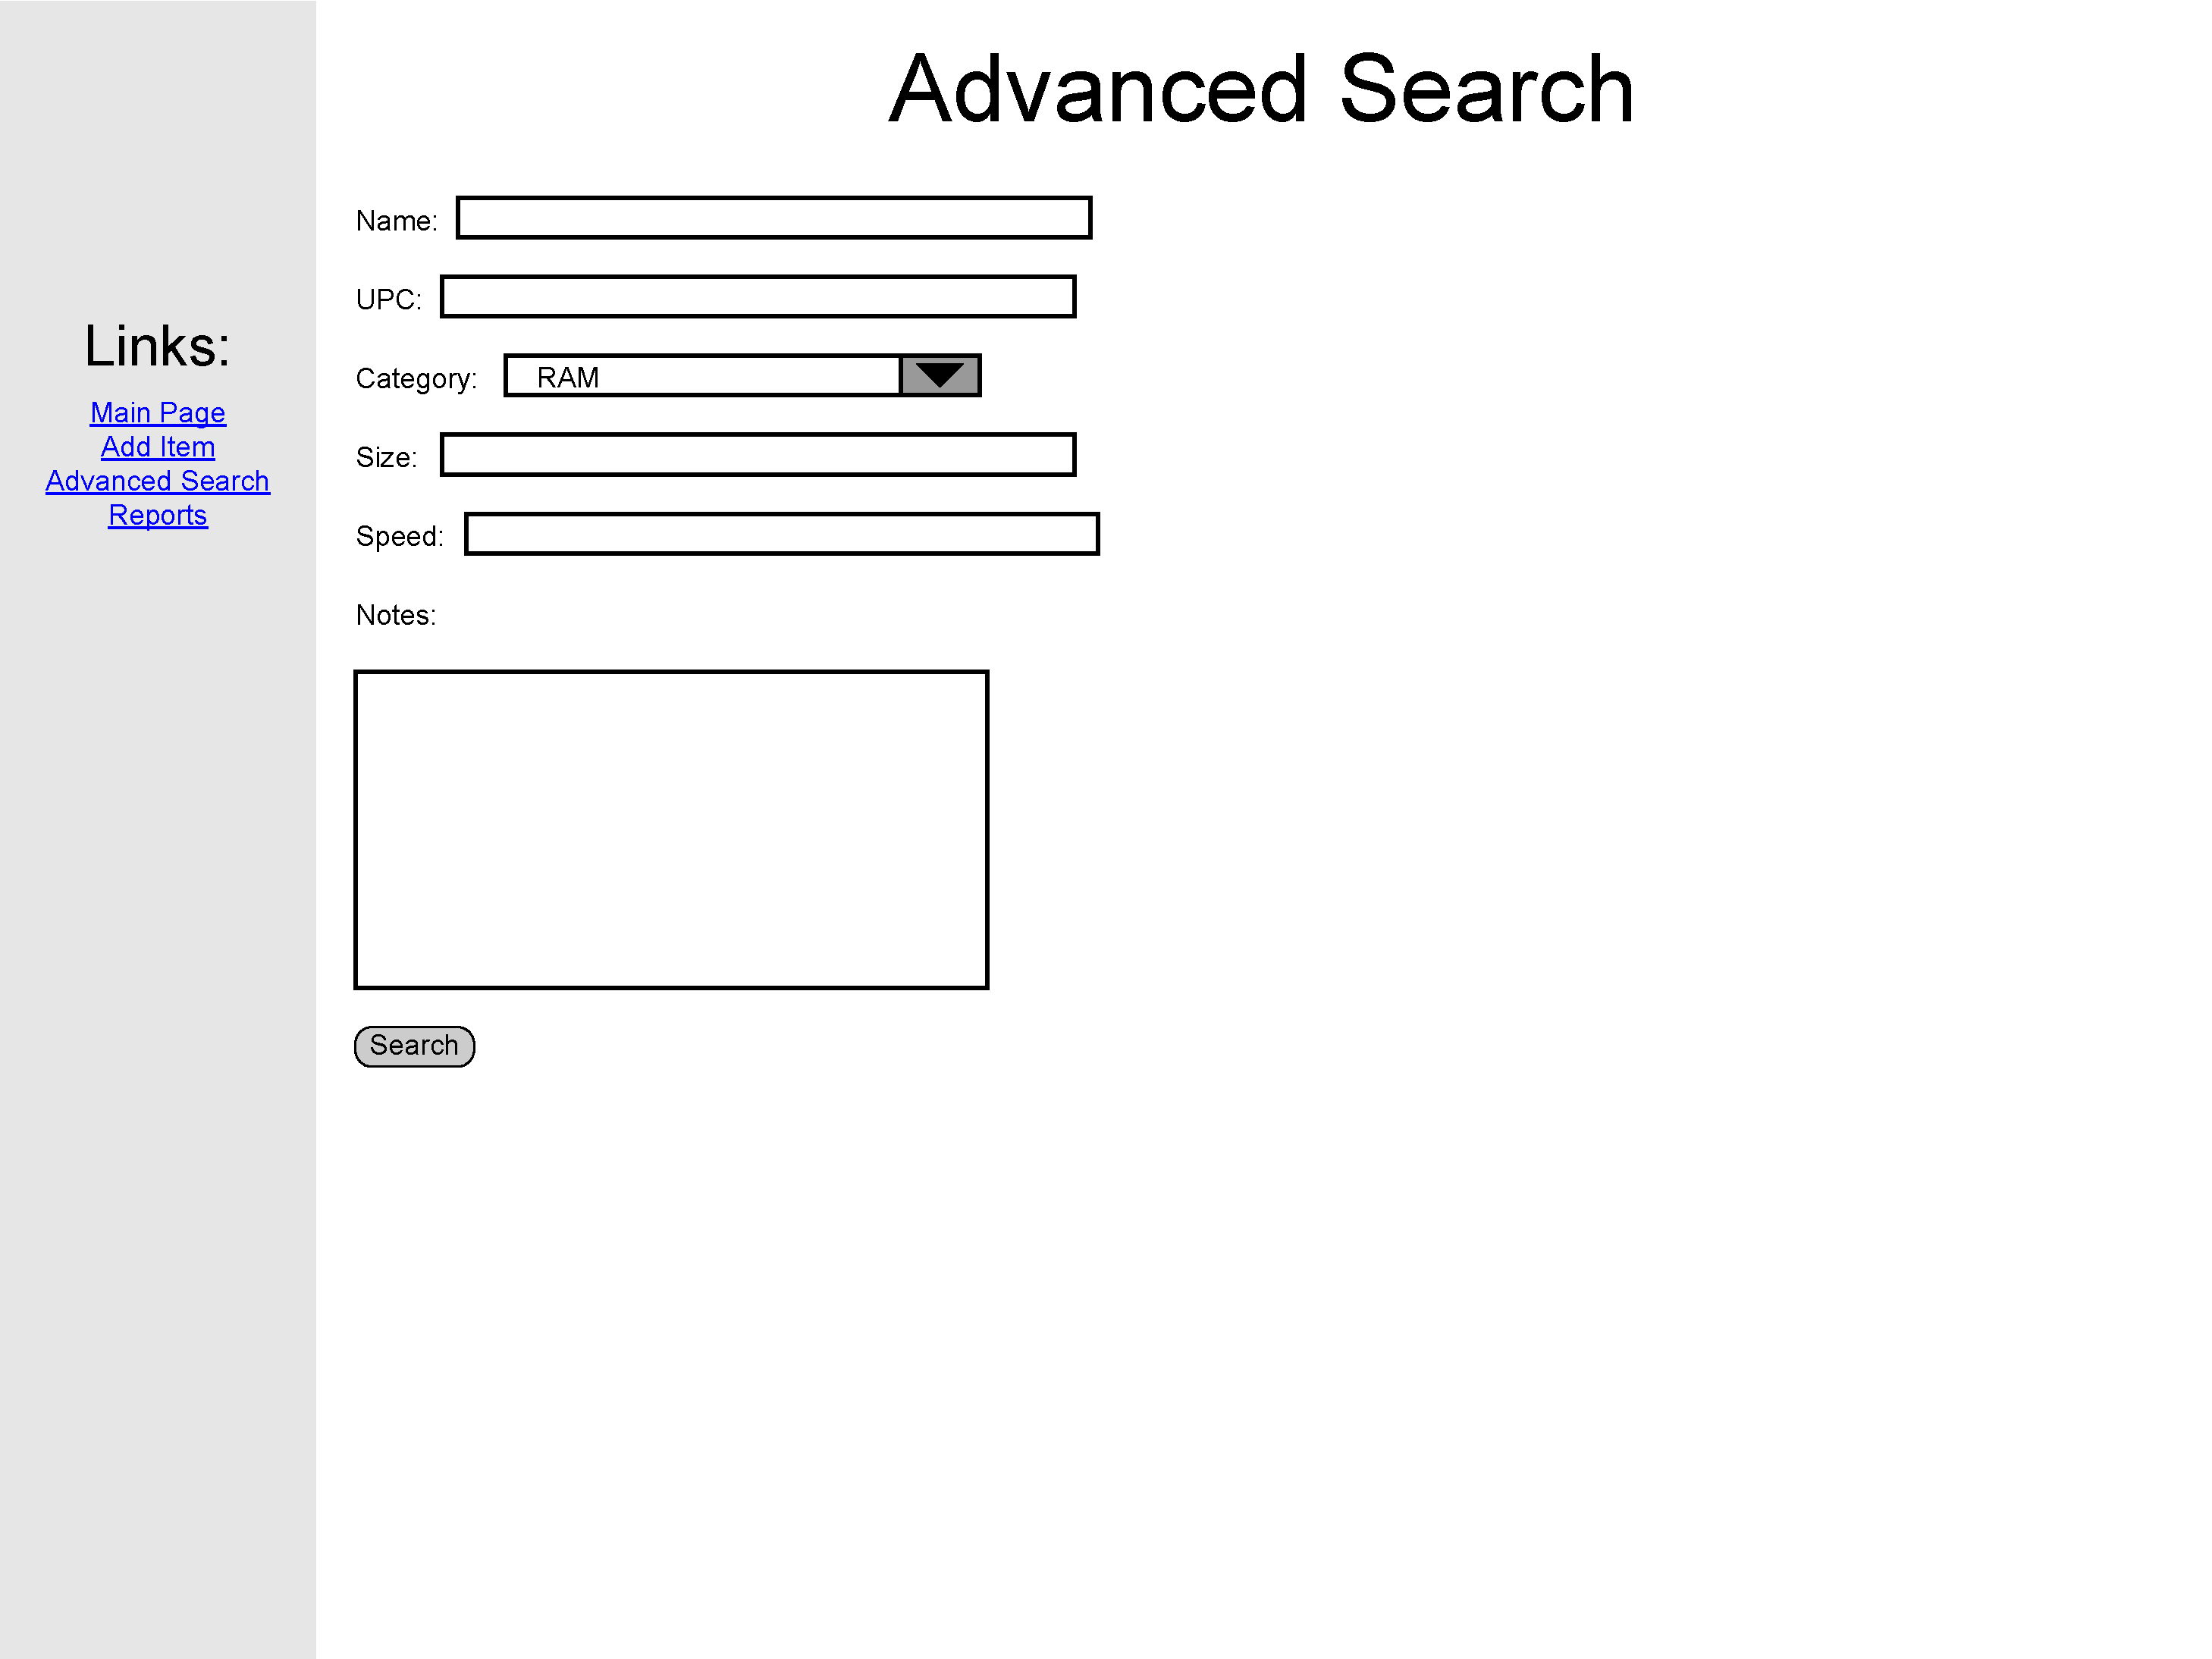
\includegraphics[keepaspectratio, width=4.5in]{advancedSearchF0S2.pdf} \\
The advanced search page with a category selected
\end{tabular}\\
~\\
~\\
\begin{tabular}{ p{4.5in} }
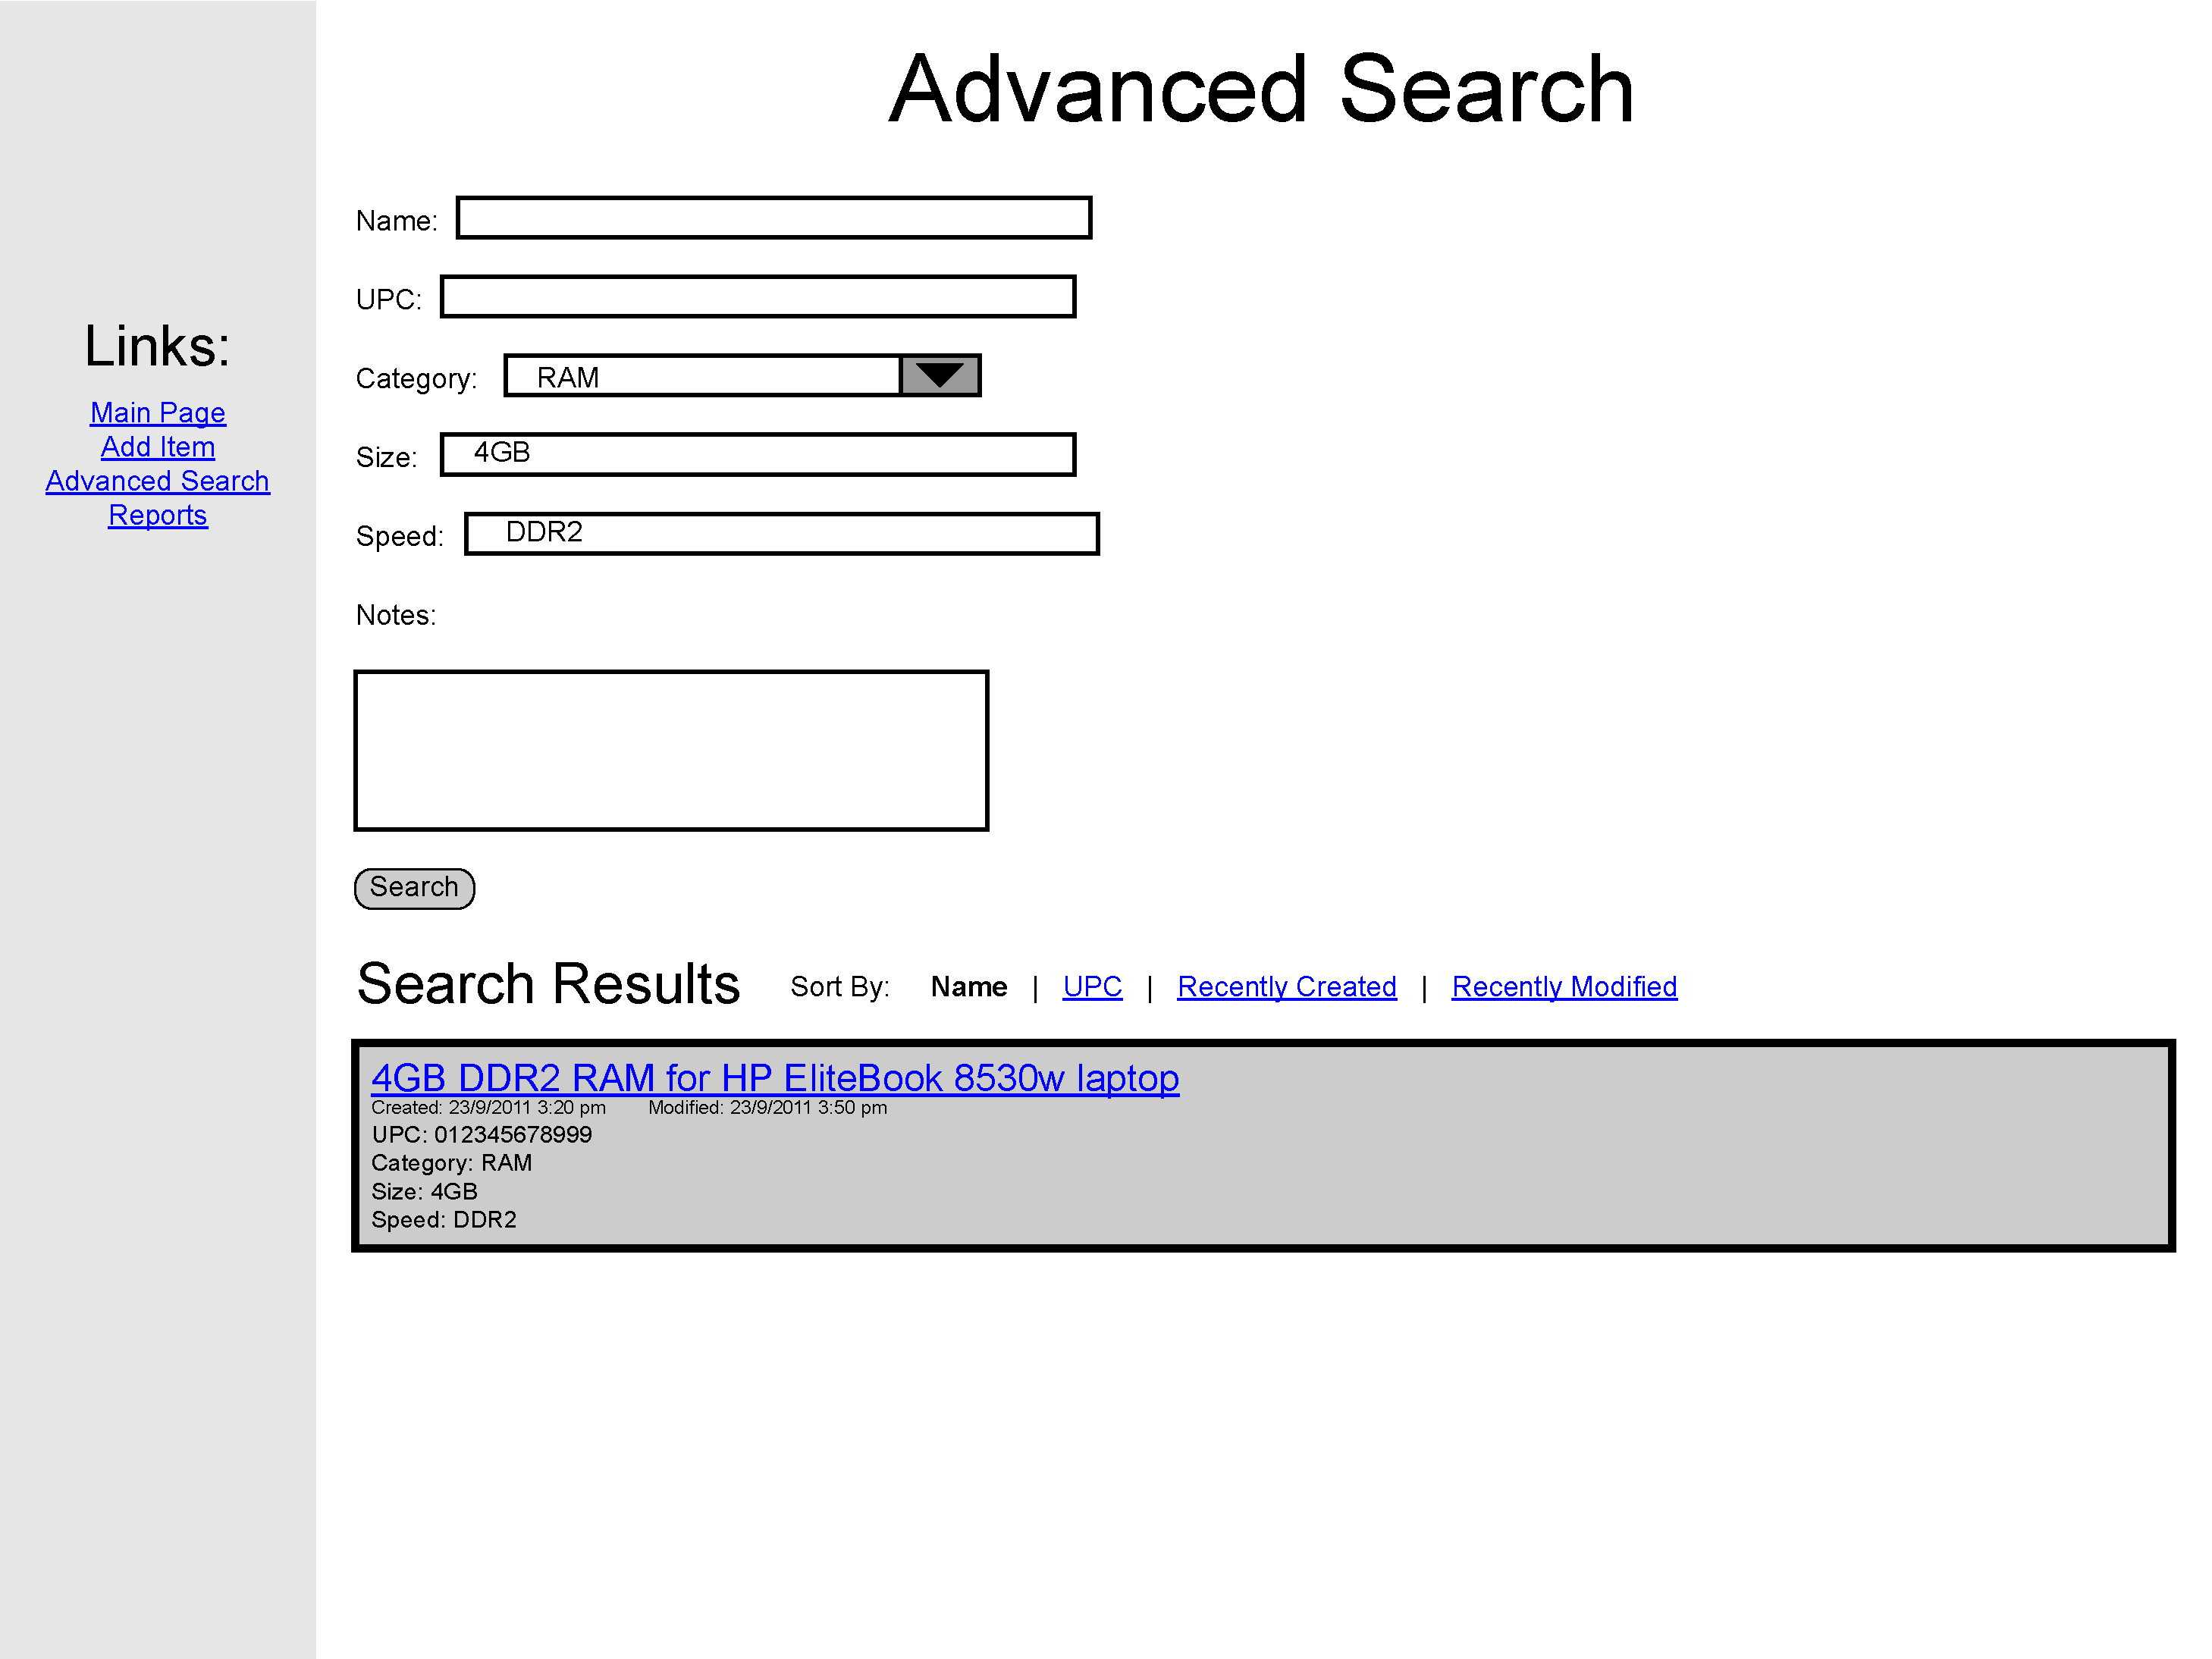
\includegraphics[keepaspectratio, width=4.5in]{advancedSearchF0S3.pdf} \\
The advanced search page with results showing
\end{tabular}\\
~\\
~\\
\begin{tabular}{ p{4.5in} }
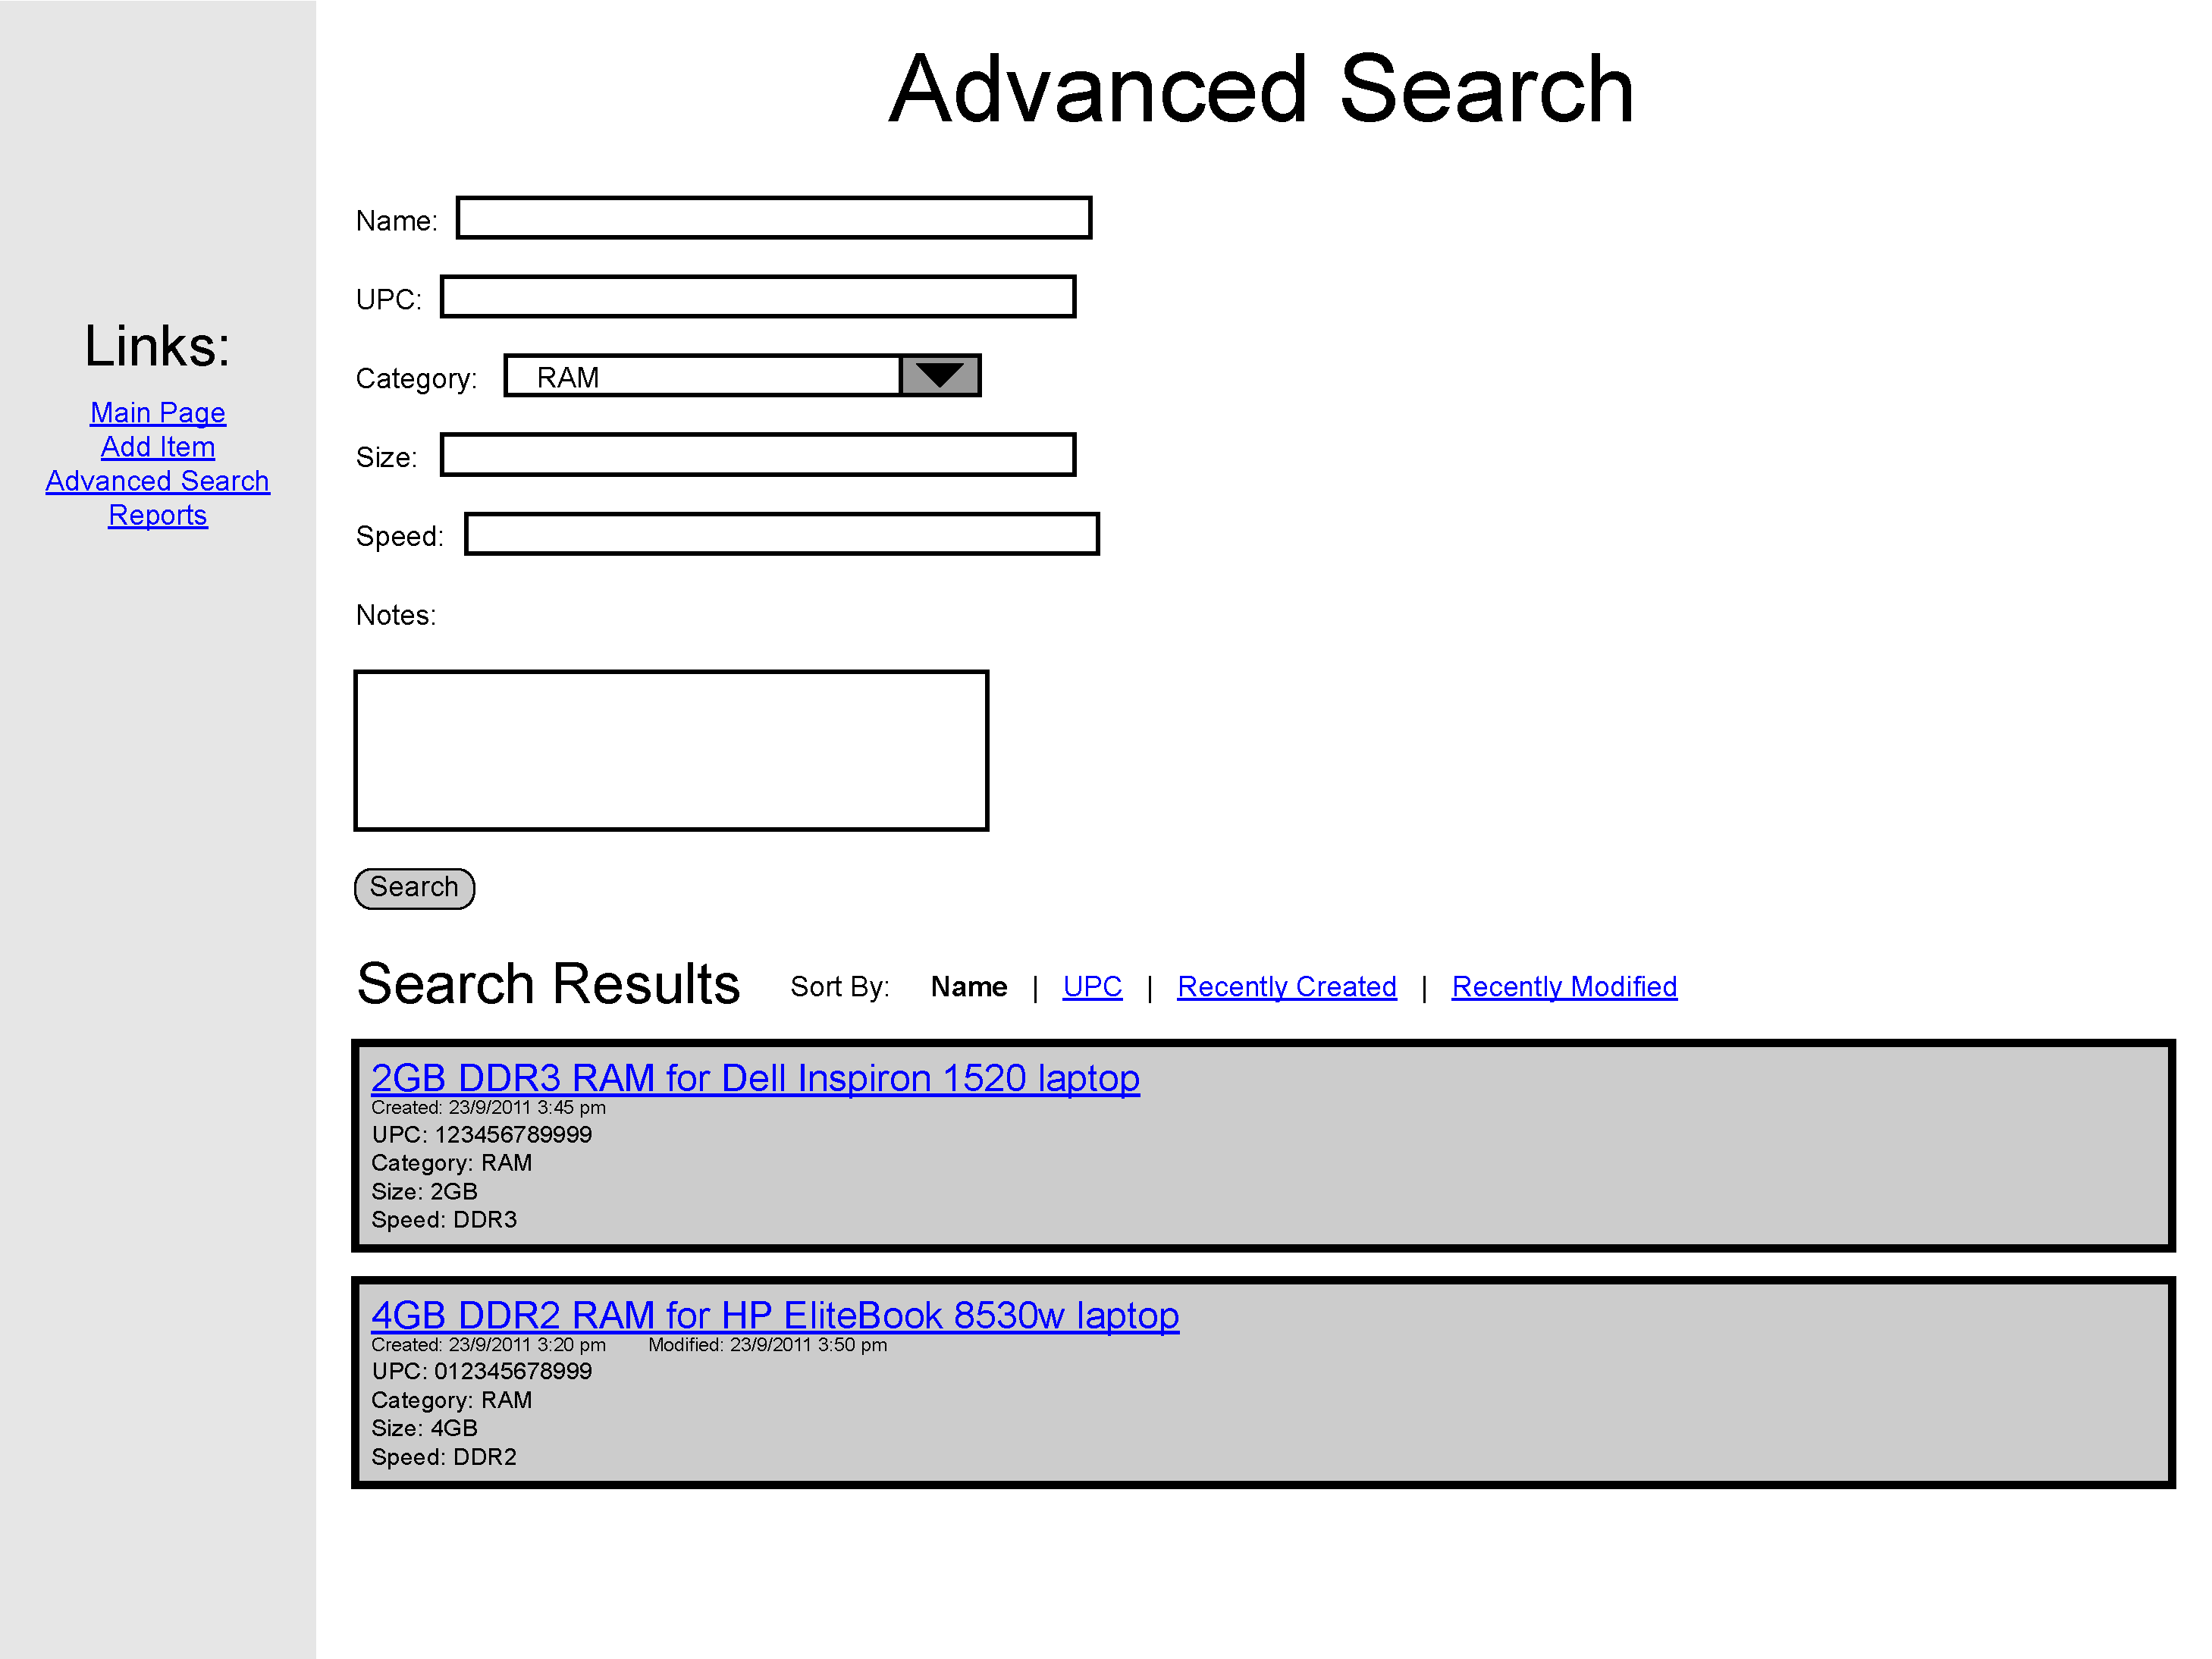
\includegraphics[keepaspectratio, width=4.5in]{sortResultsF0S0.pdf} \\
The advanced search page with results sorted by the default of Name
\end{tabular}\\
~\\
~\\
\begin{tabular}{ p{4.5in} }
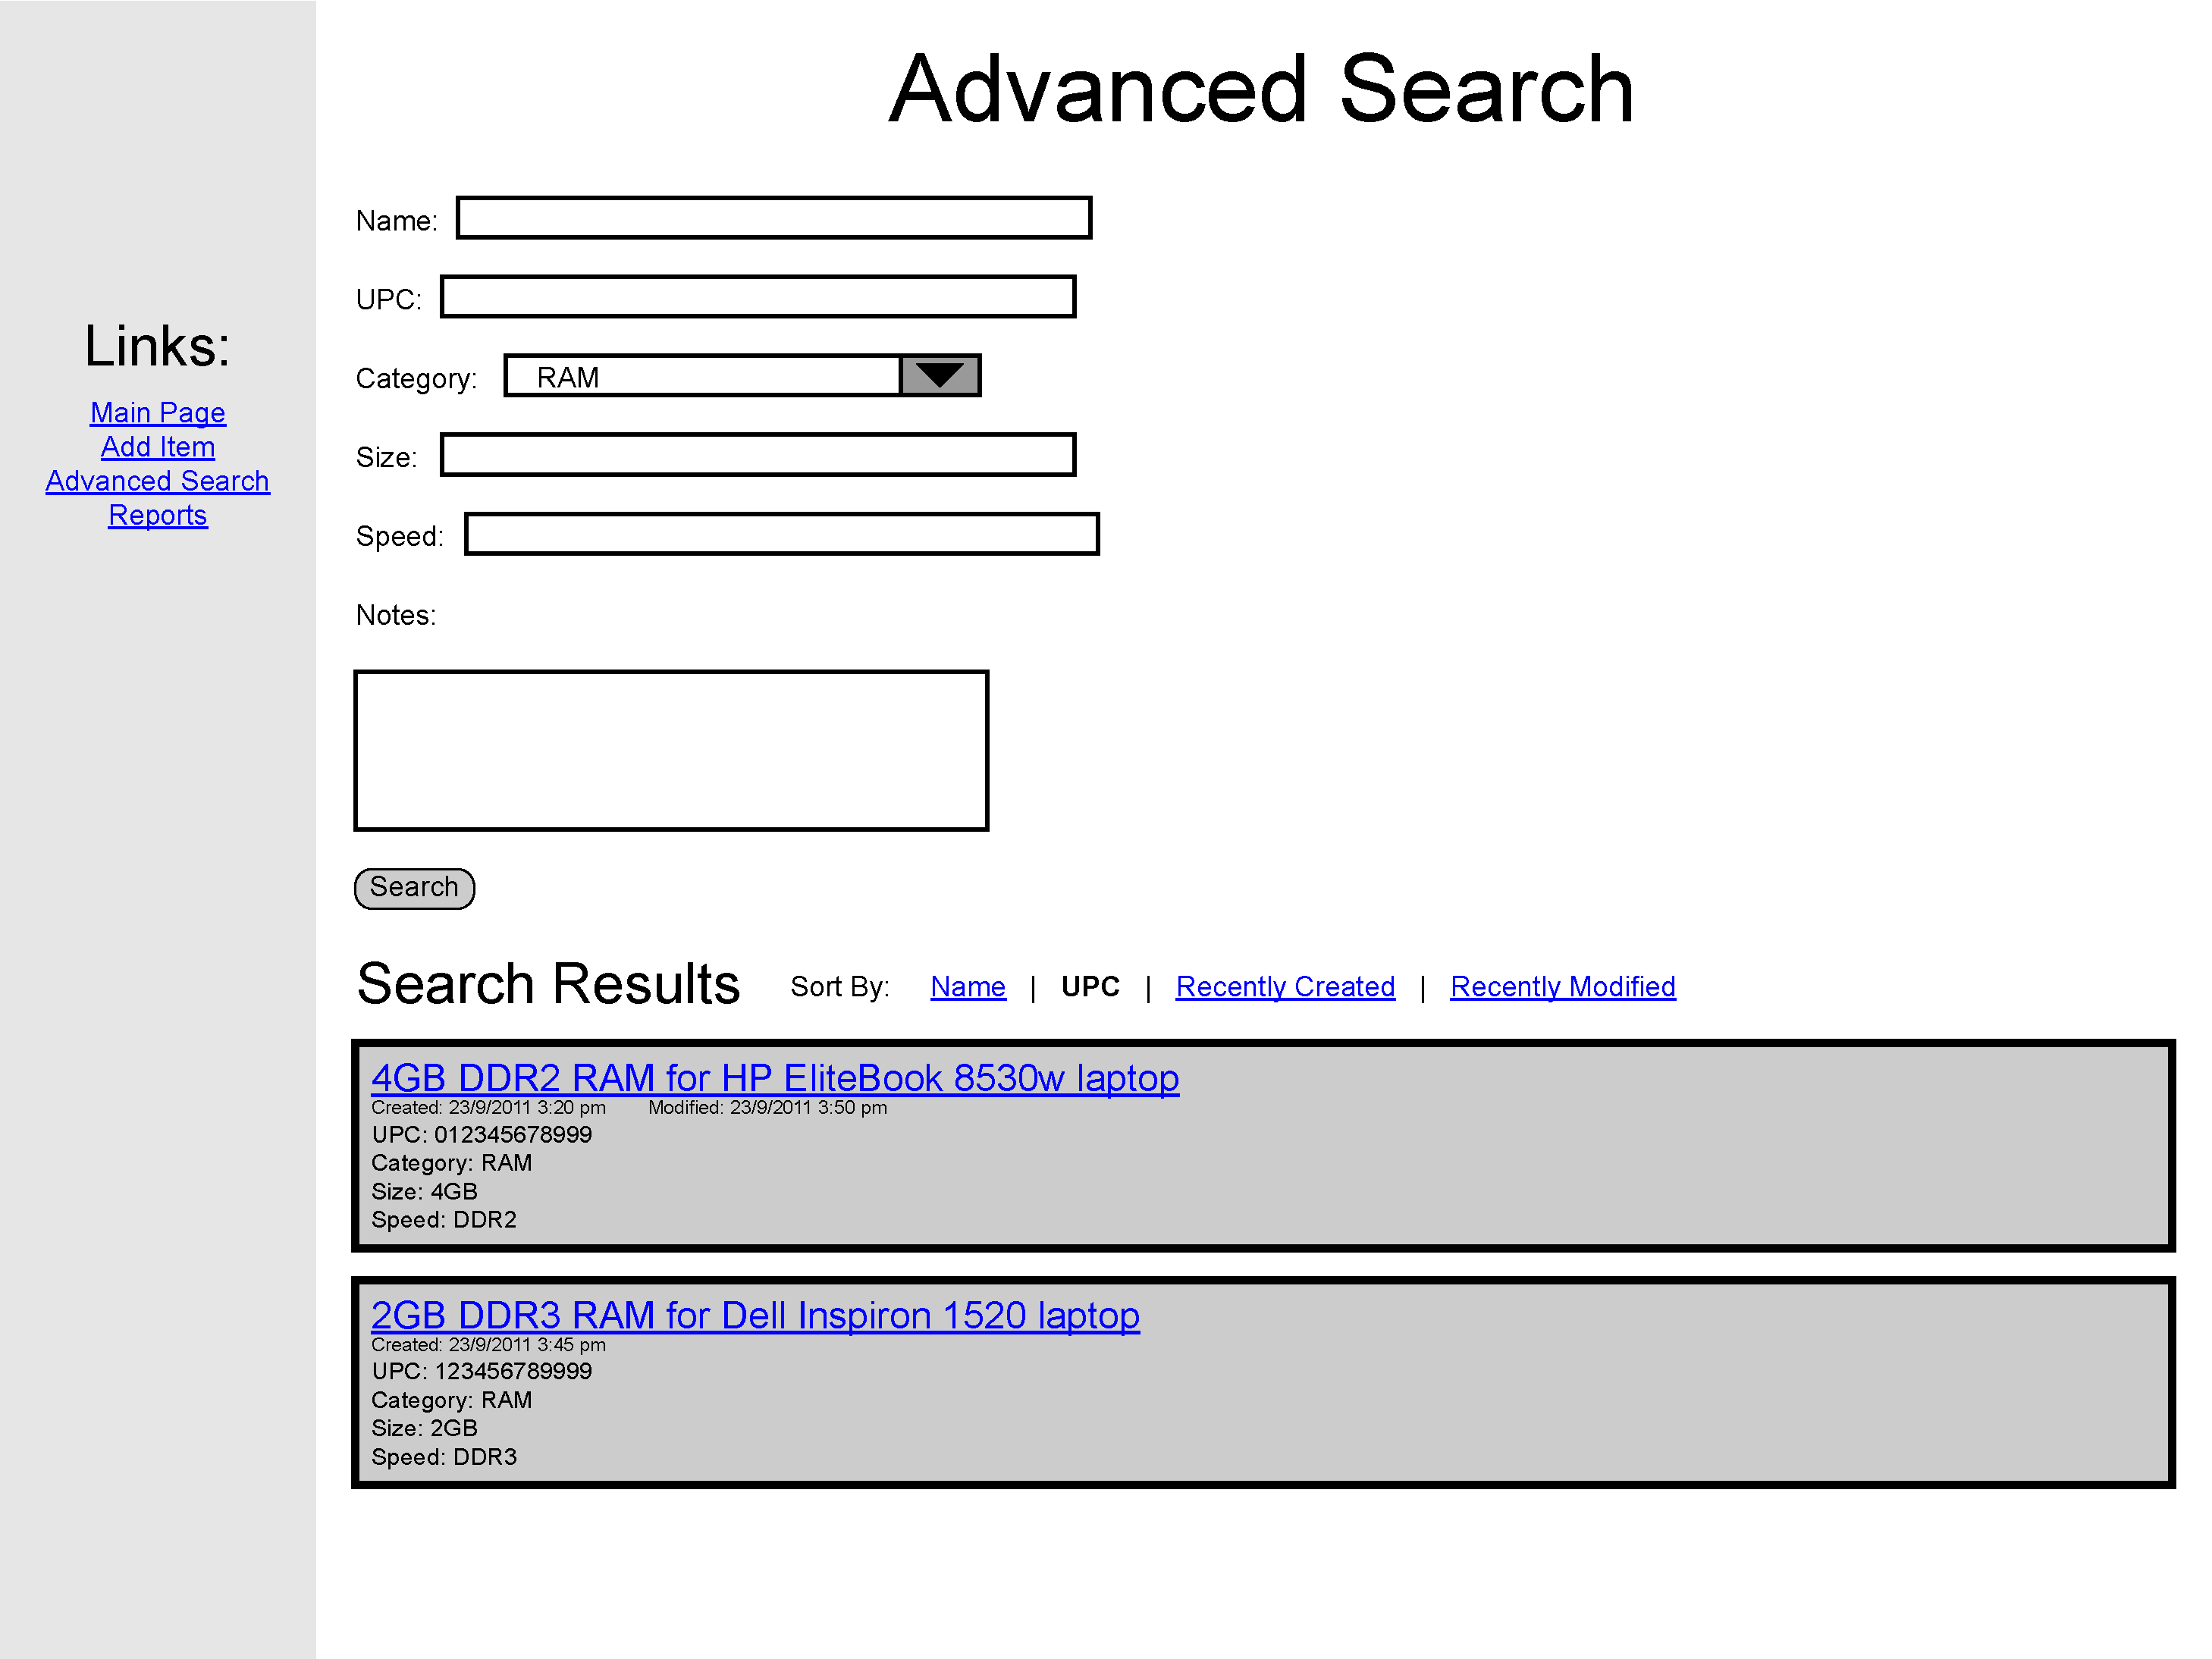
\includegraphics[keepaspectratio, width=4.5in]{sortResultsF0S1.pdf} \\
The advanced search page with results sorted by the user's choice of UPC
\end{tabular}\\
~\\
~\\
\begin{tabular}{ p{4.5in} }
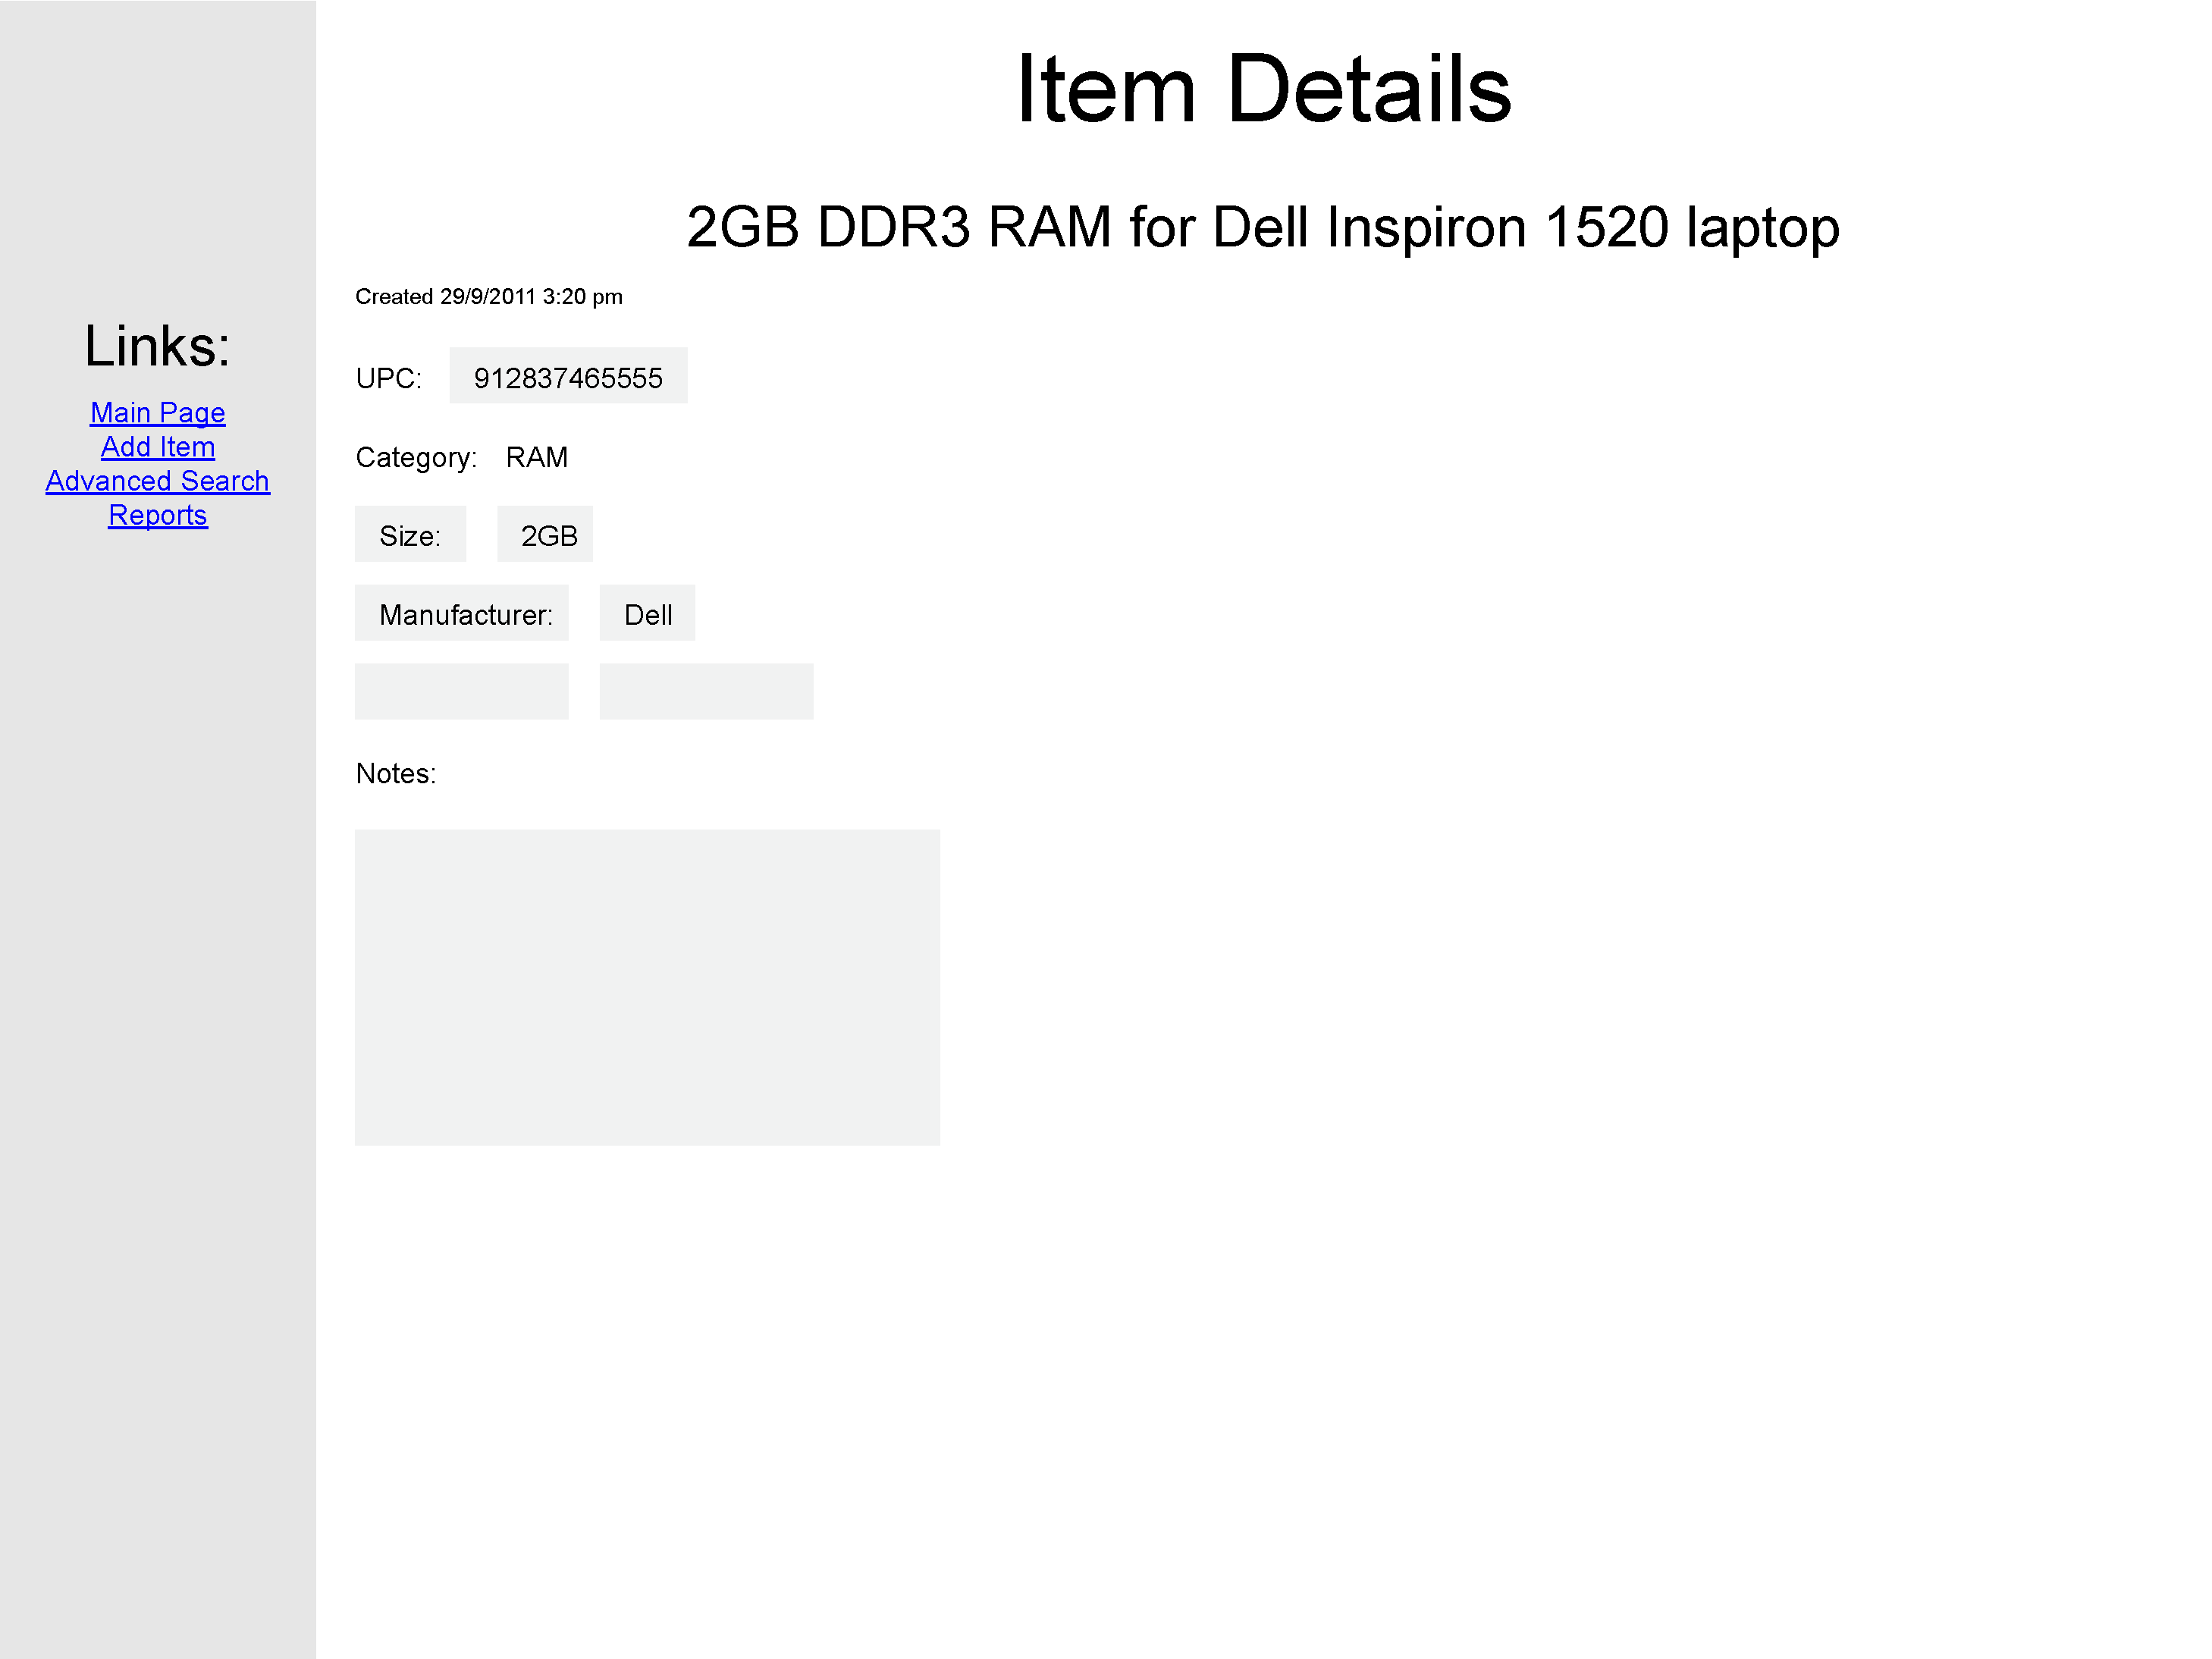
\includegraphics[keepaspectratio, width=4.5in]{viewDetailsF0S1.pdf} \\
The item details page in its initial state
\end{tabular}\\
~\\
~\\
\begin{tabular}{ p{4.5in} }
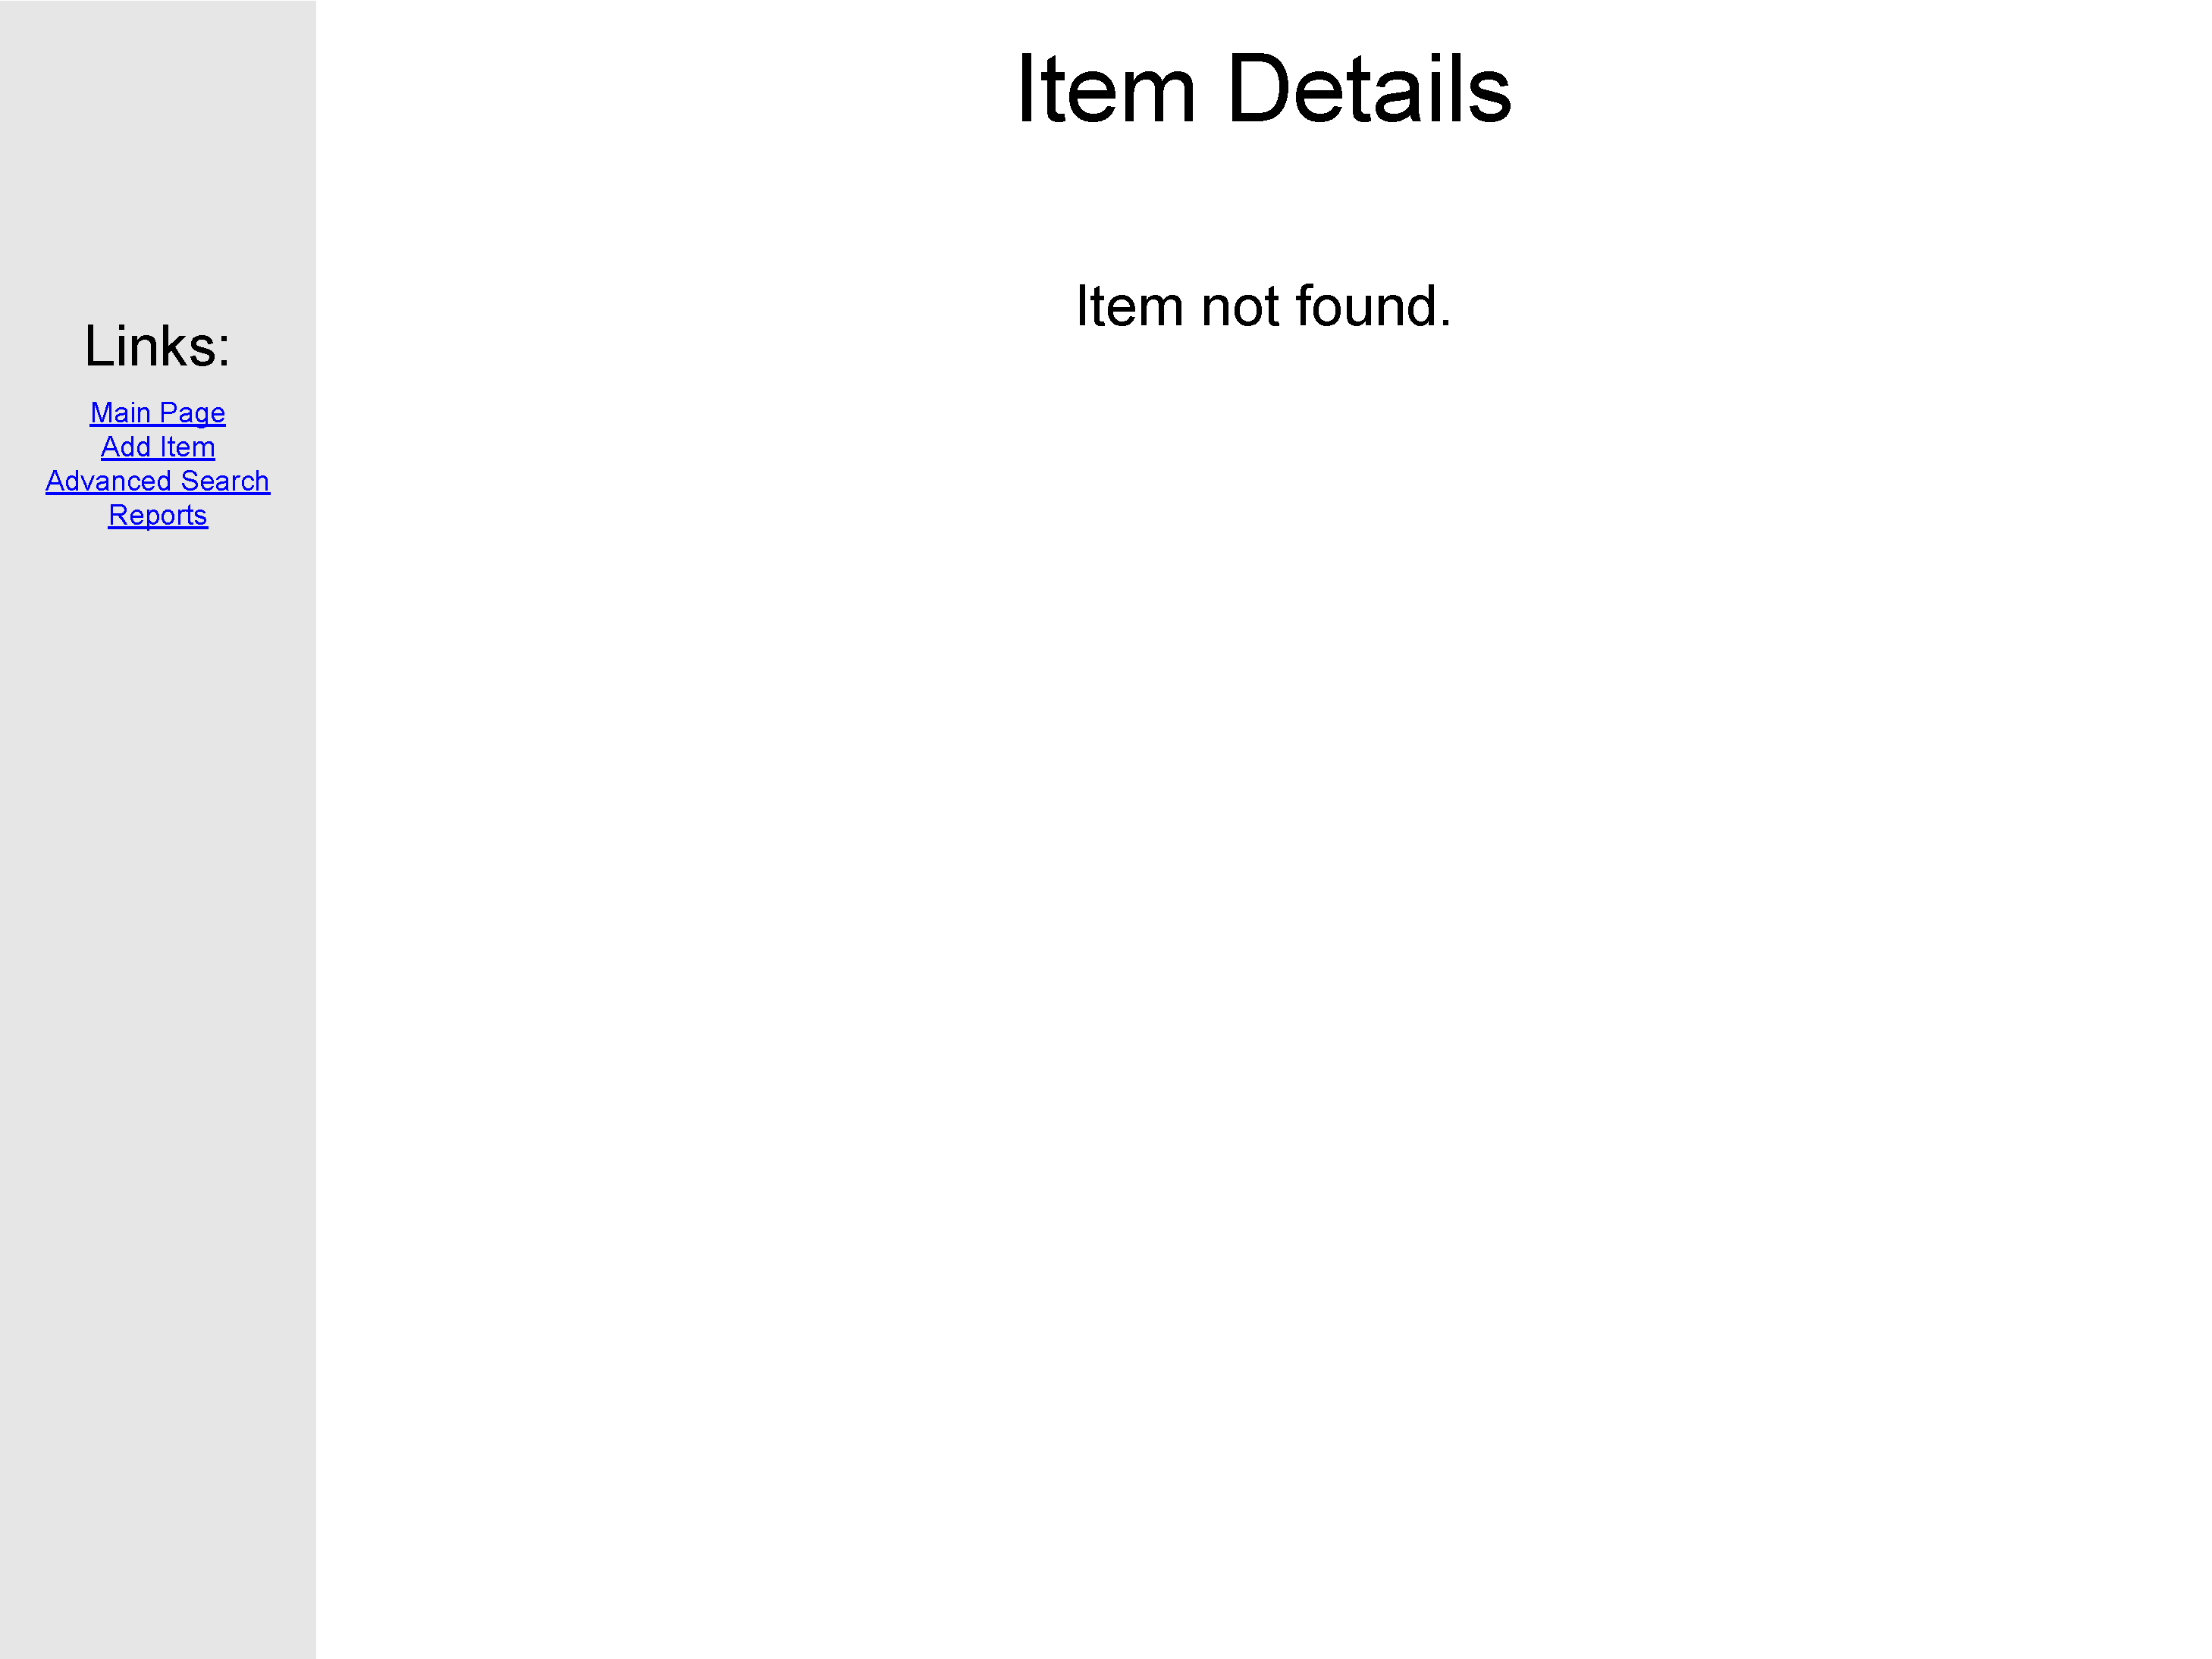
\includegraphics[keepaspectratio, width=4.5in]{viewDetailsF1S1.pdf} \\
The item details page for an item that could not be found.
\end{tabular}\\
~\\
~\\
\begin{tabular}{ p{4.5in} }
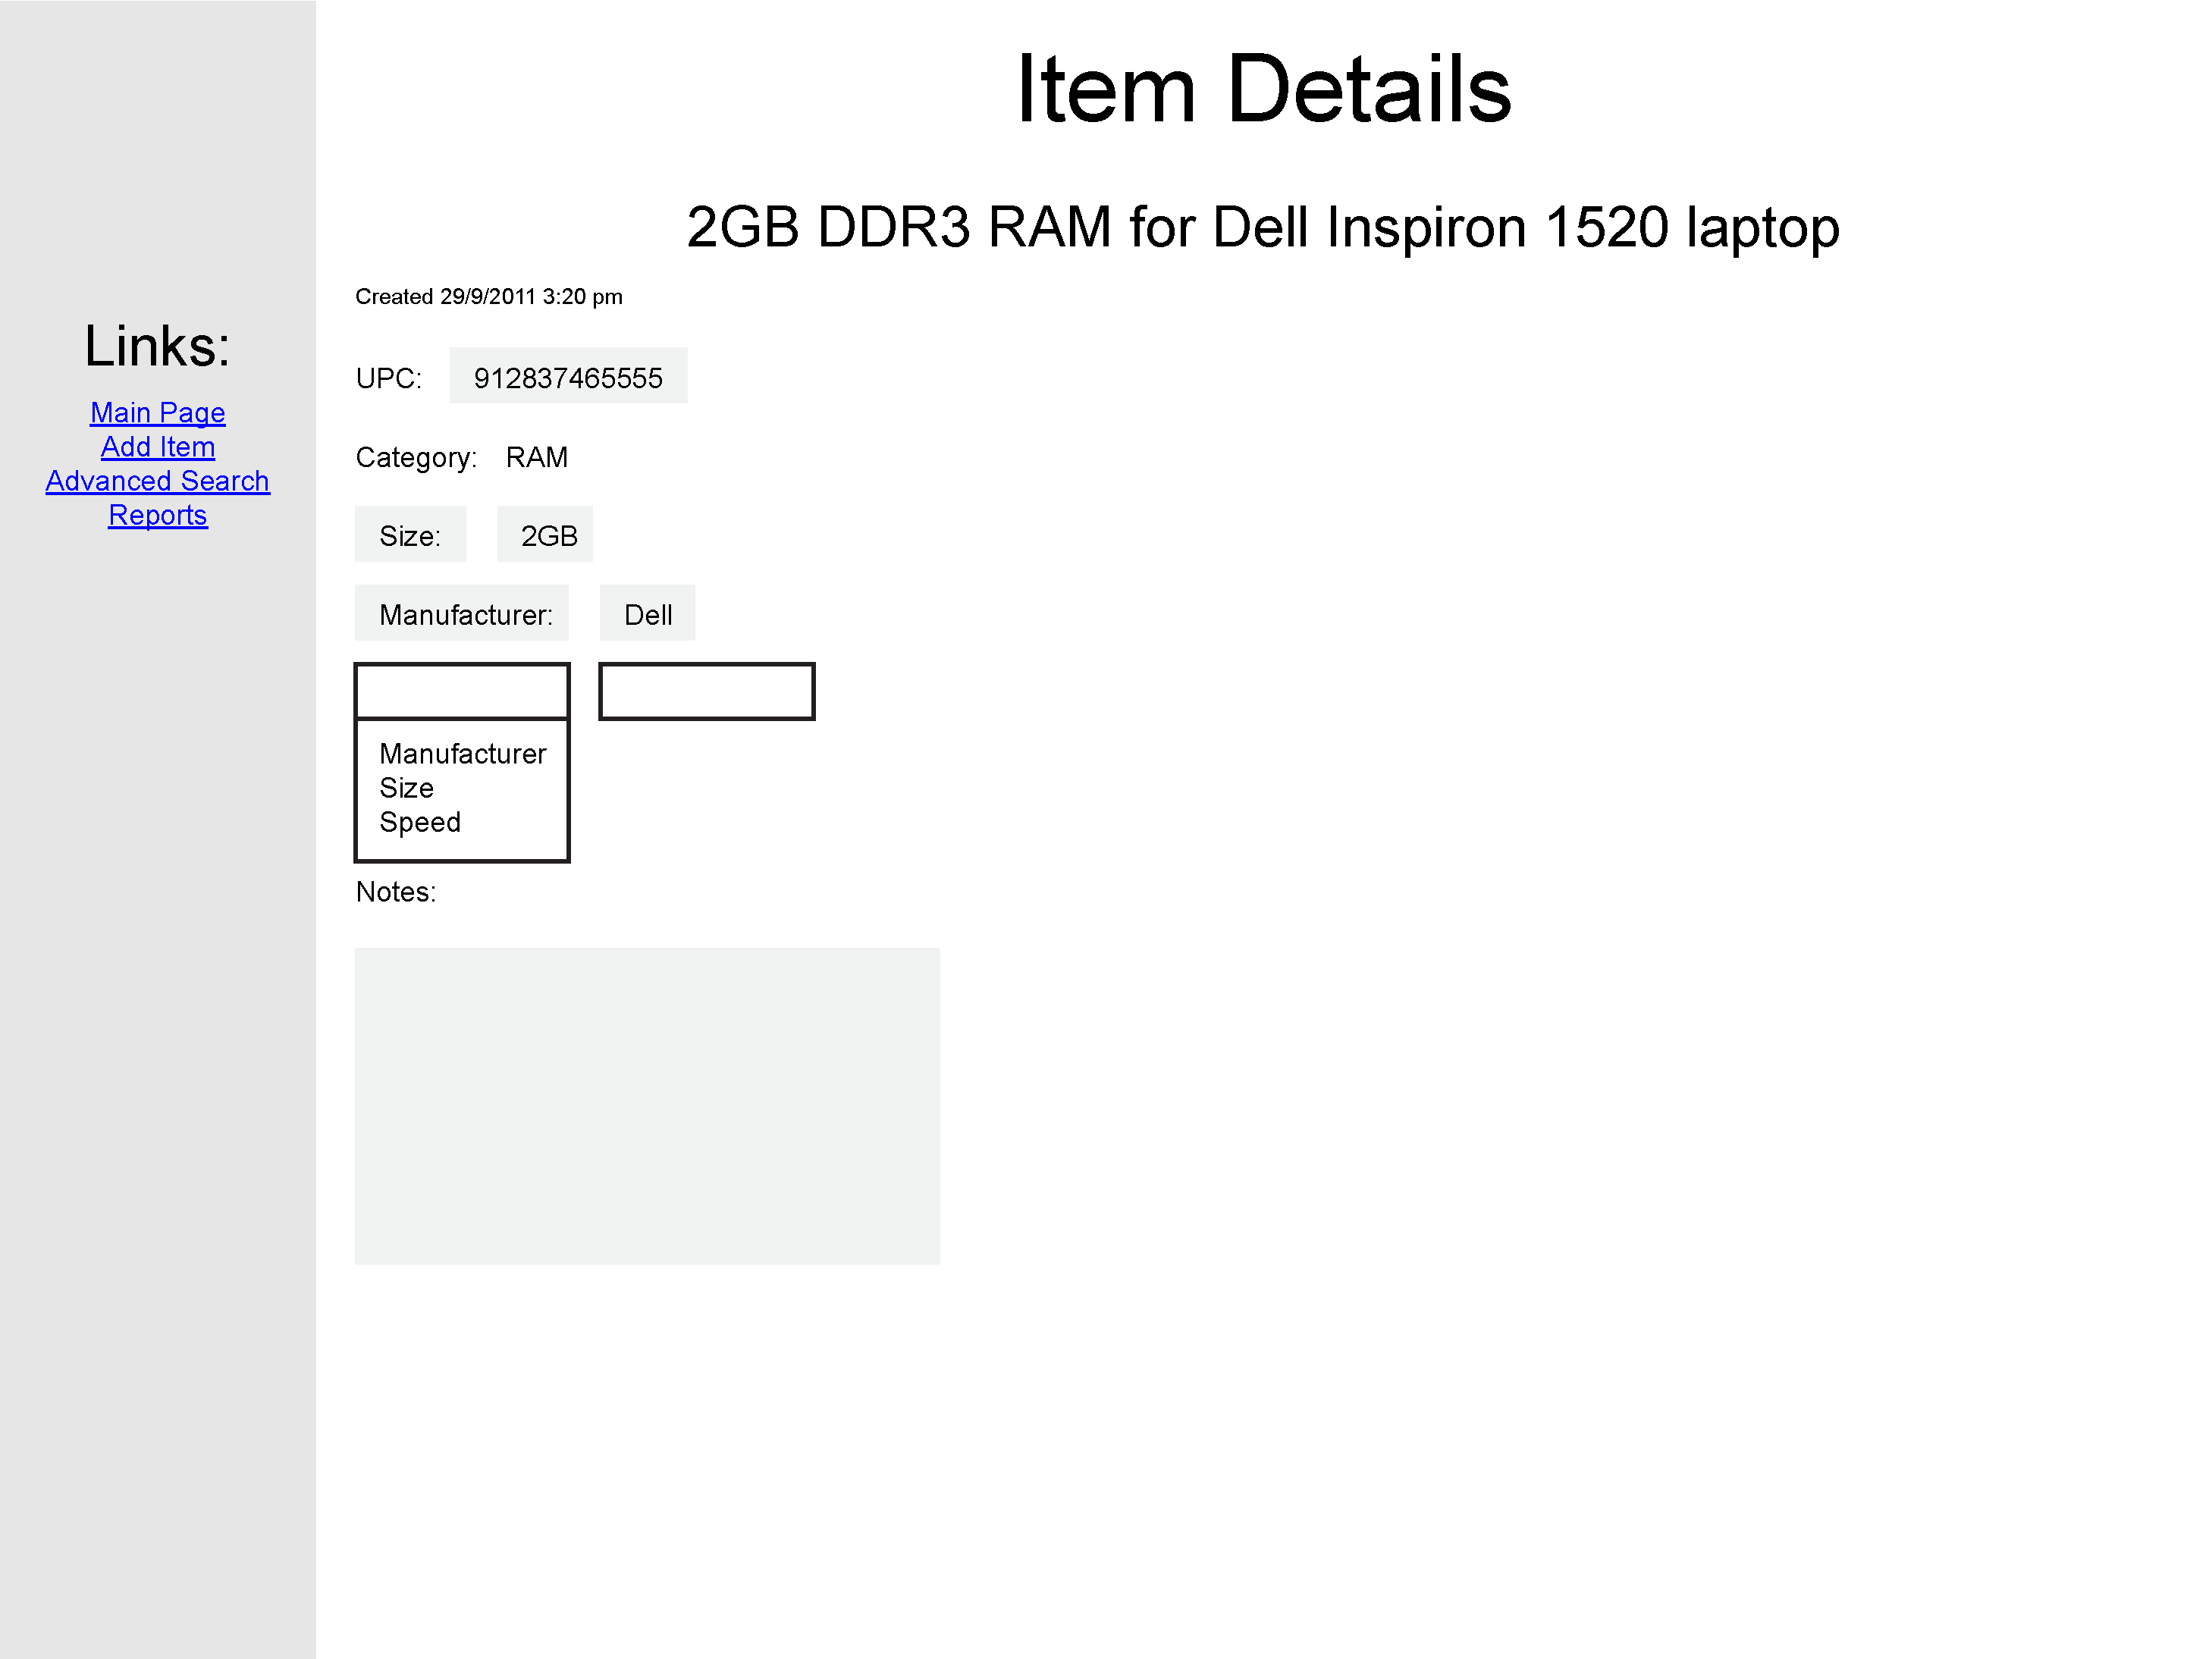
\includegraphics[keepaspectratio, width=4.5in]{modifyDetailsF0S1.pdf} \\
The item details page after the user has clicked on the empty attribute key field and caused the element to be replaced with an autocomplete text field
\end{tabular}\\
~\\
~\\
\begin{tabular}{ p{4.5in} }
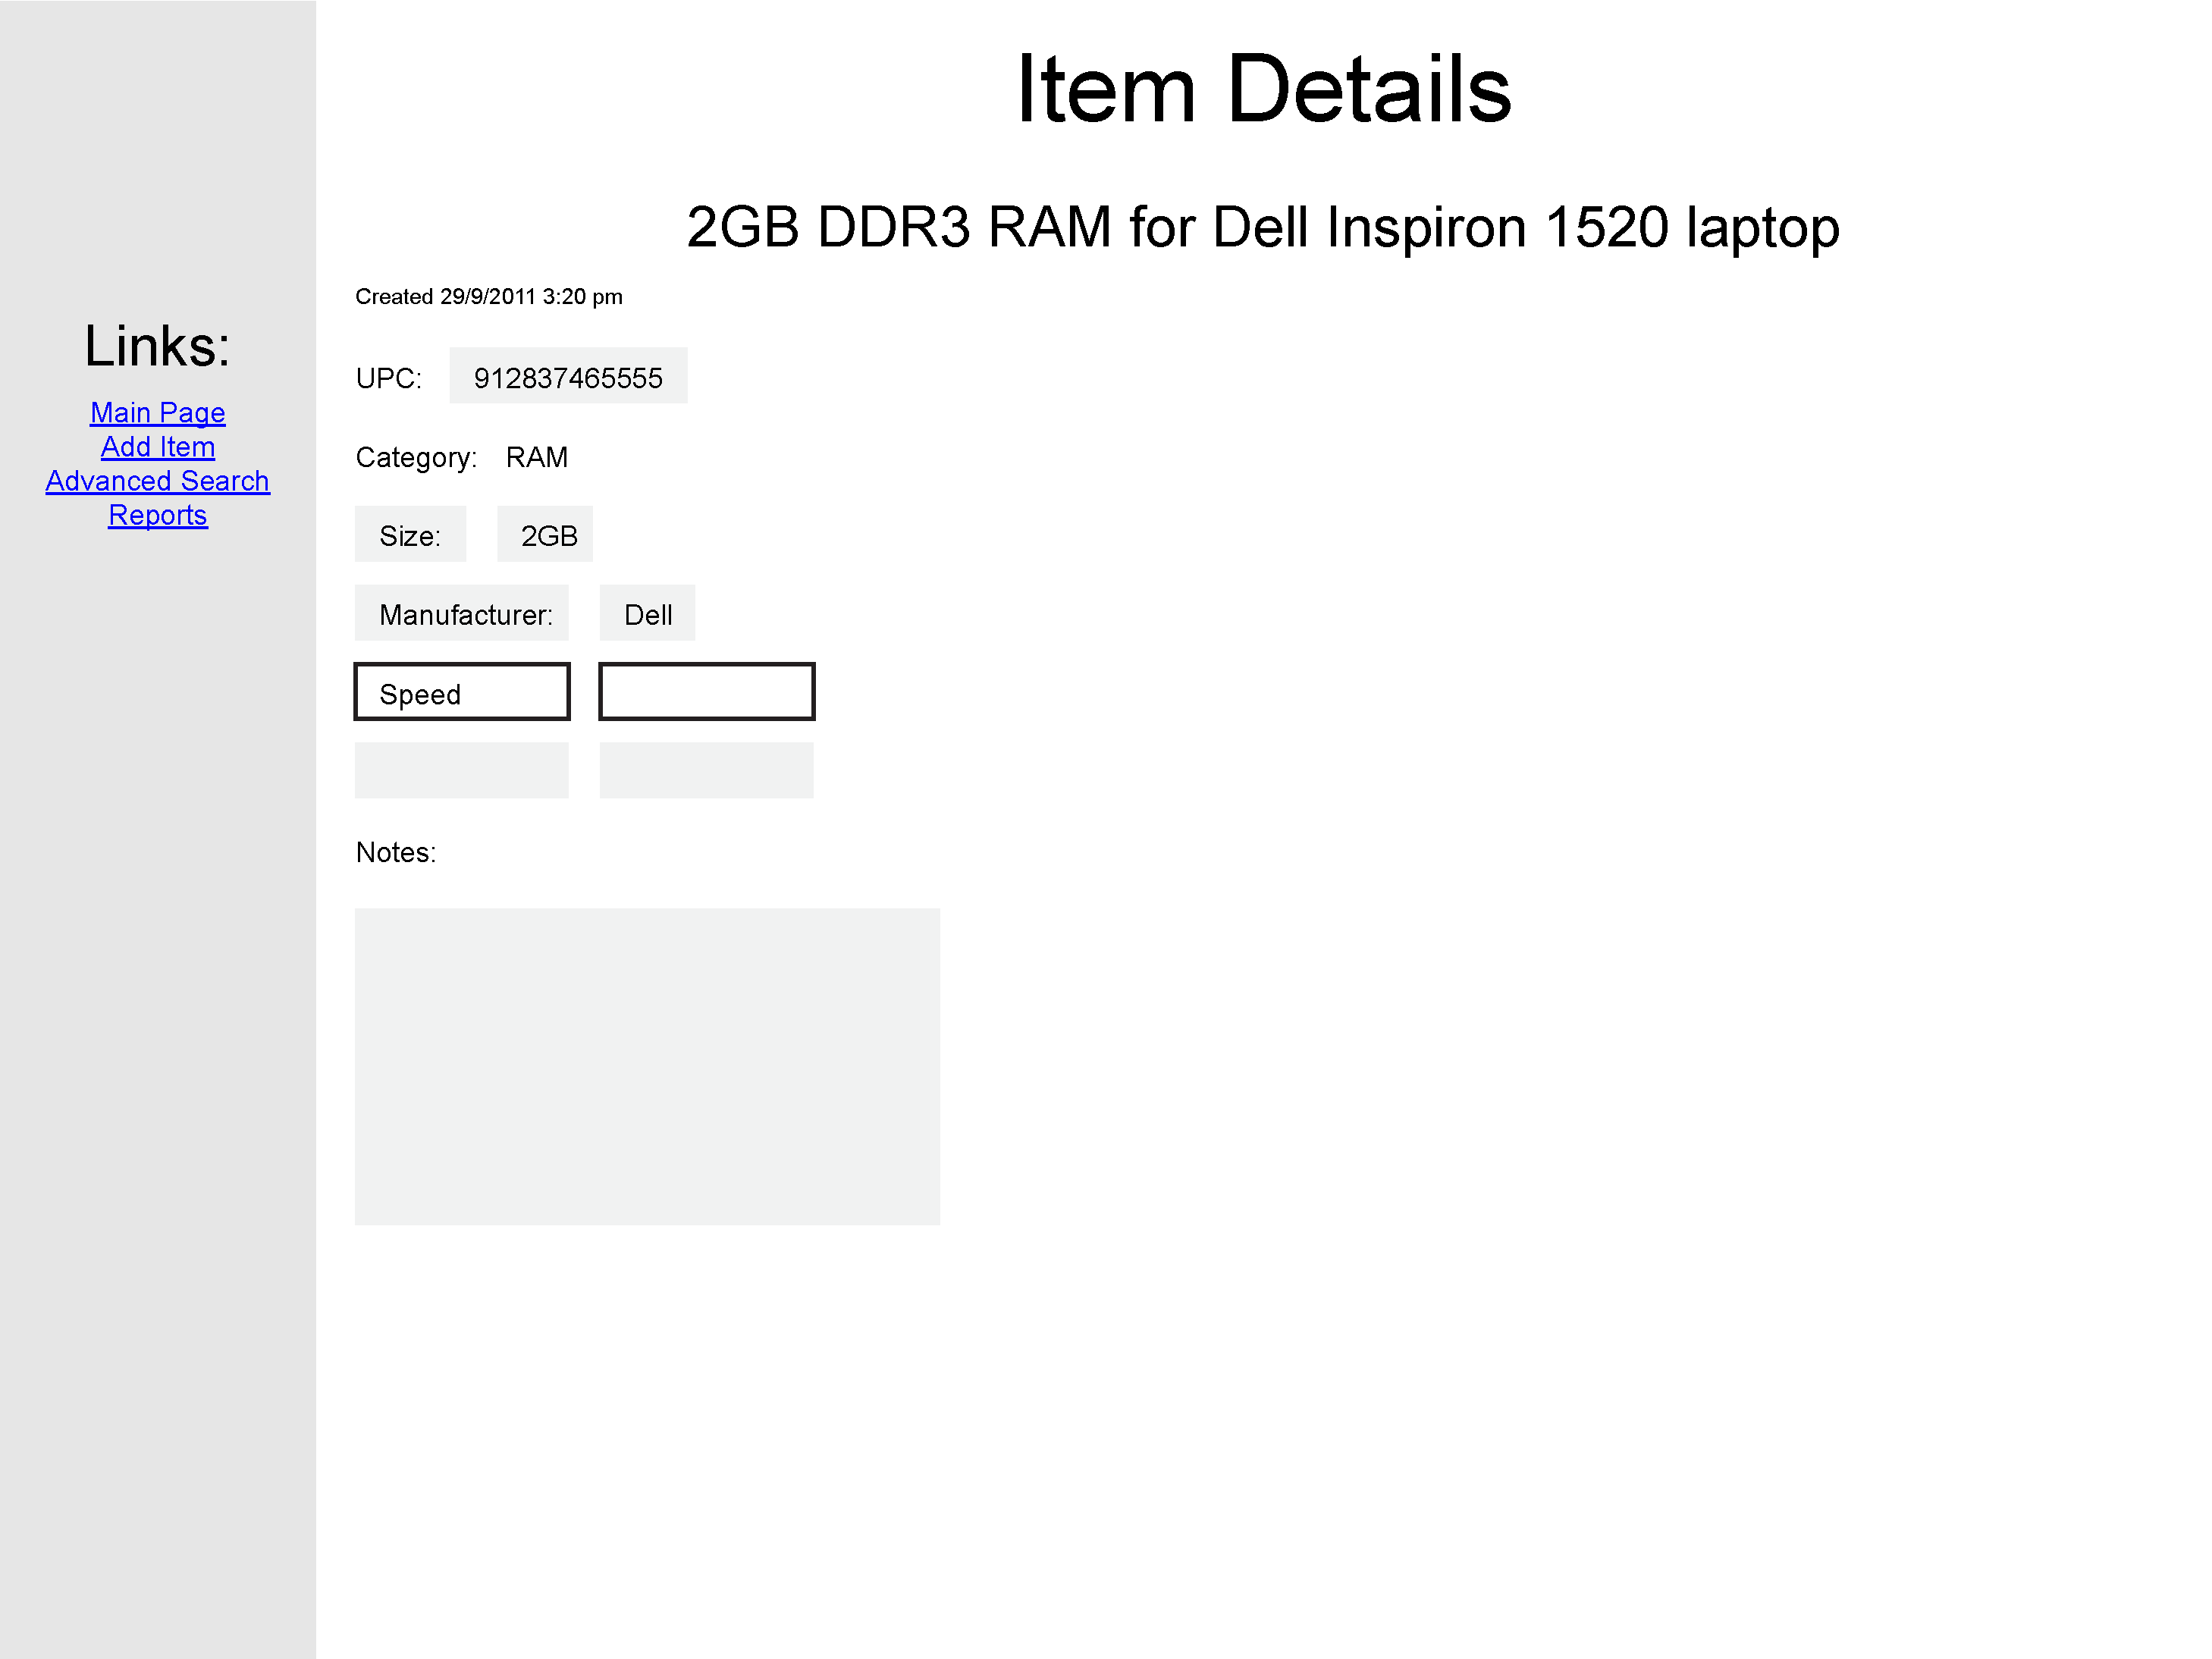
\includegraphics[keepaspectratio, width=4.5in]{modifyDetailsF0S2.pdf} \\
The item details page after an attribute key has been selected
\end{tabular}\\
~\\
~\\
\begin{tabular}{ p{4.5in} }
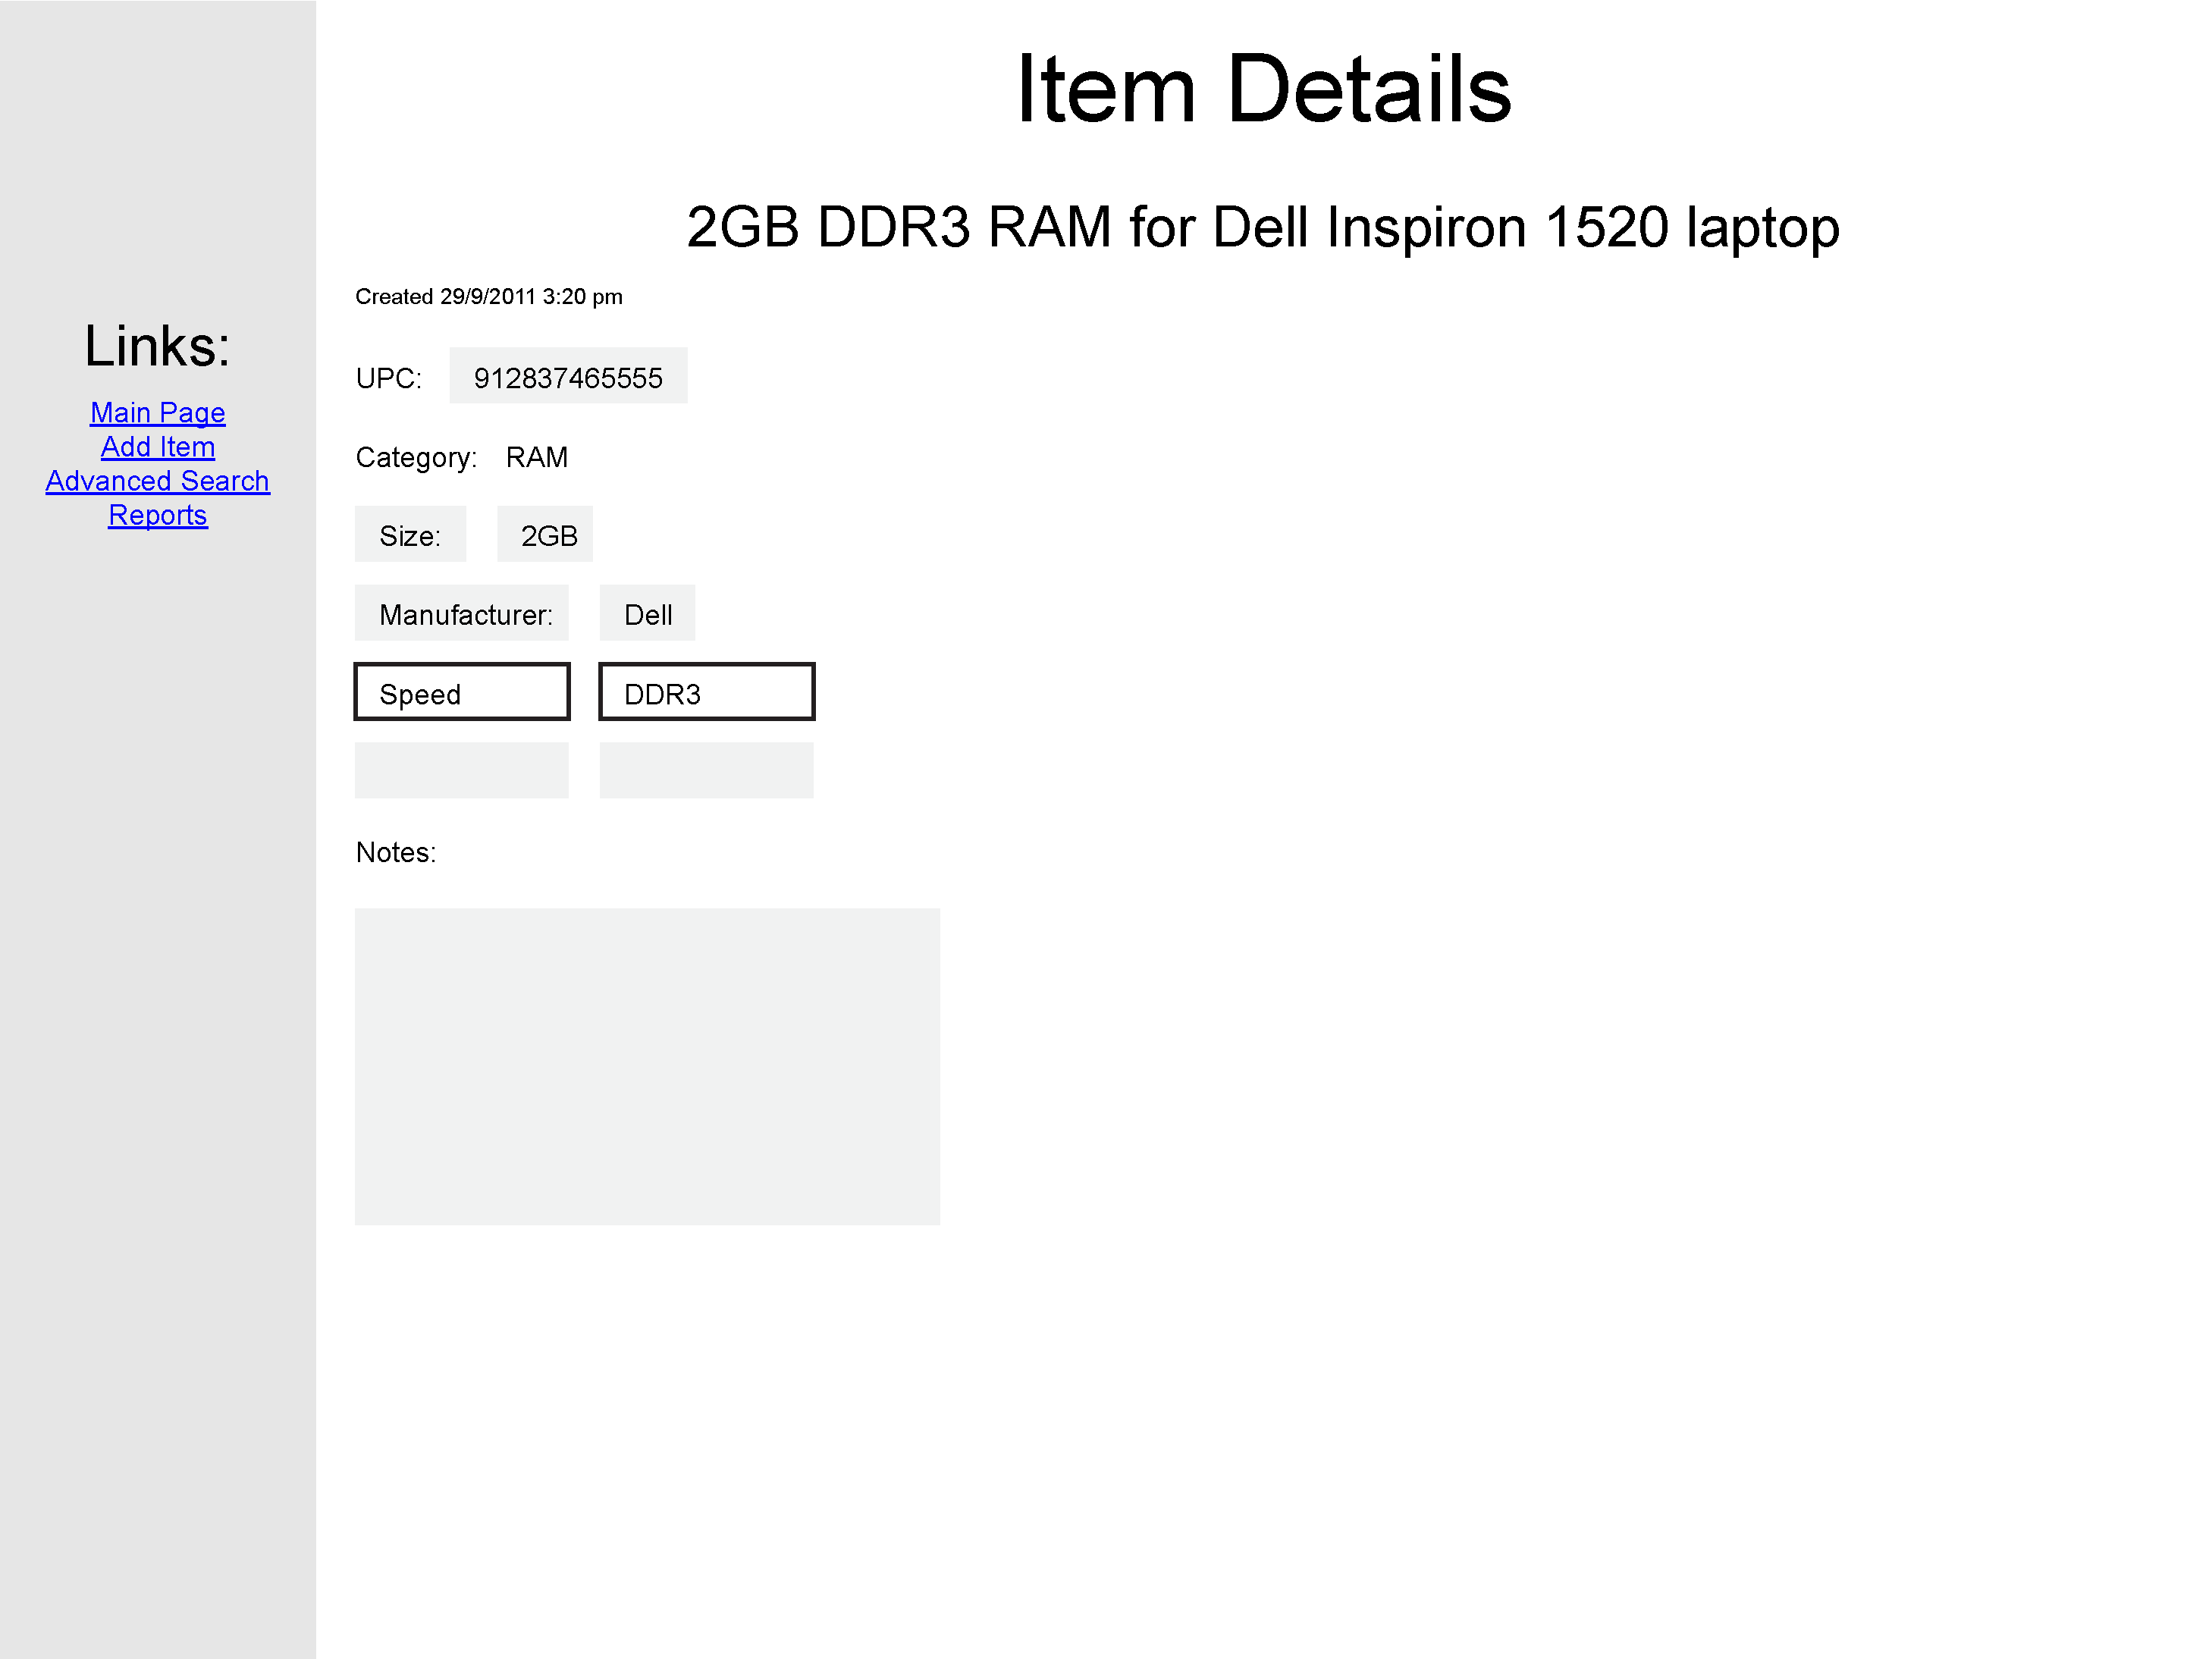
\includegraphics[keepaspectratio, width=4.5in]{modifyDetailsF0S3.pdf} \\
The item details page after the attribute key and value have been entered
\end{tabular}\\
~\\
~\\
\begin{tabular}{ p{4.5in} }
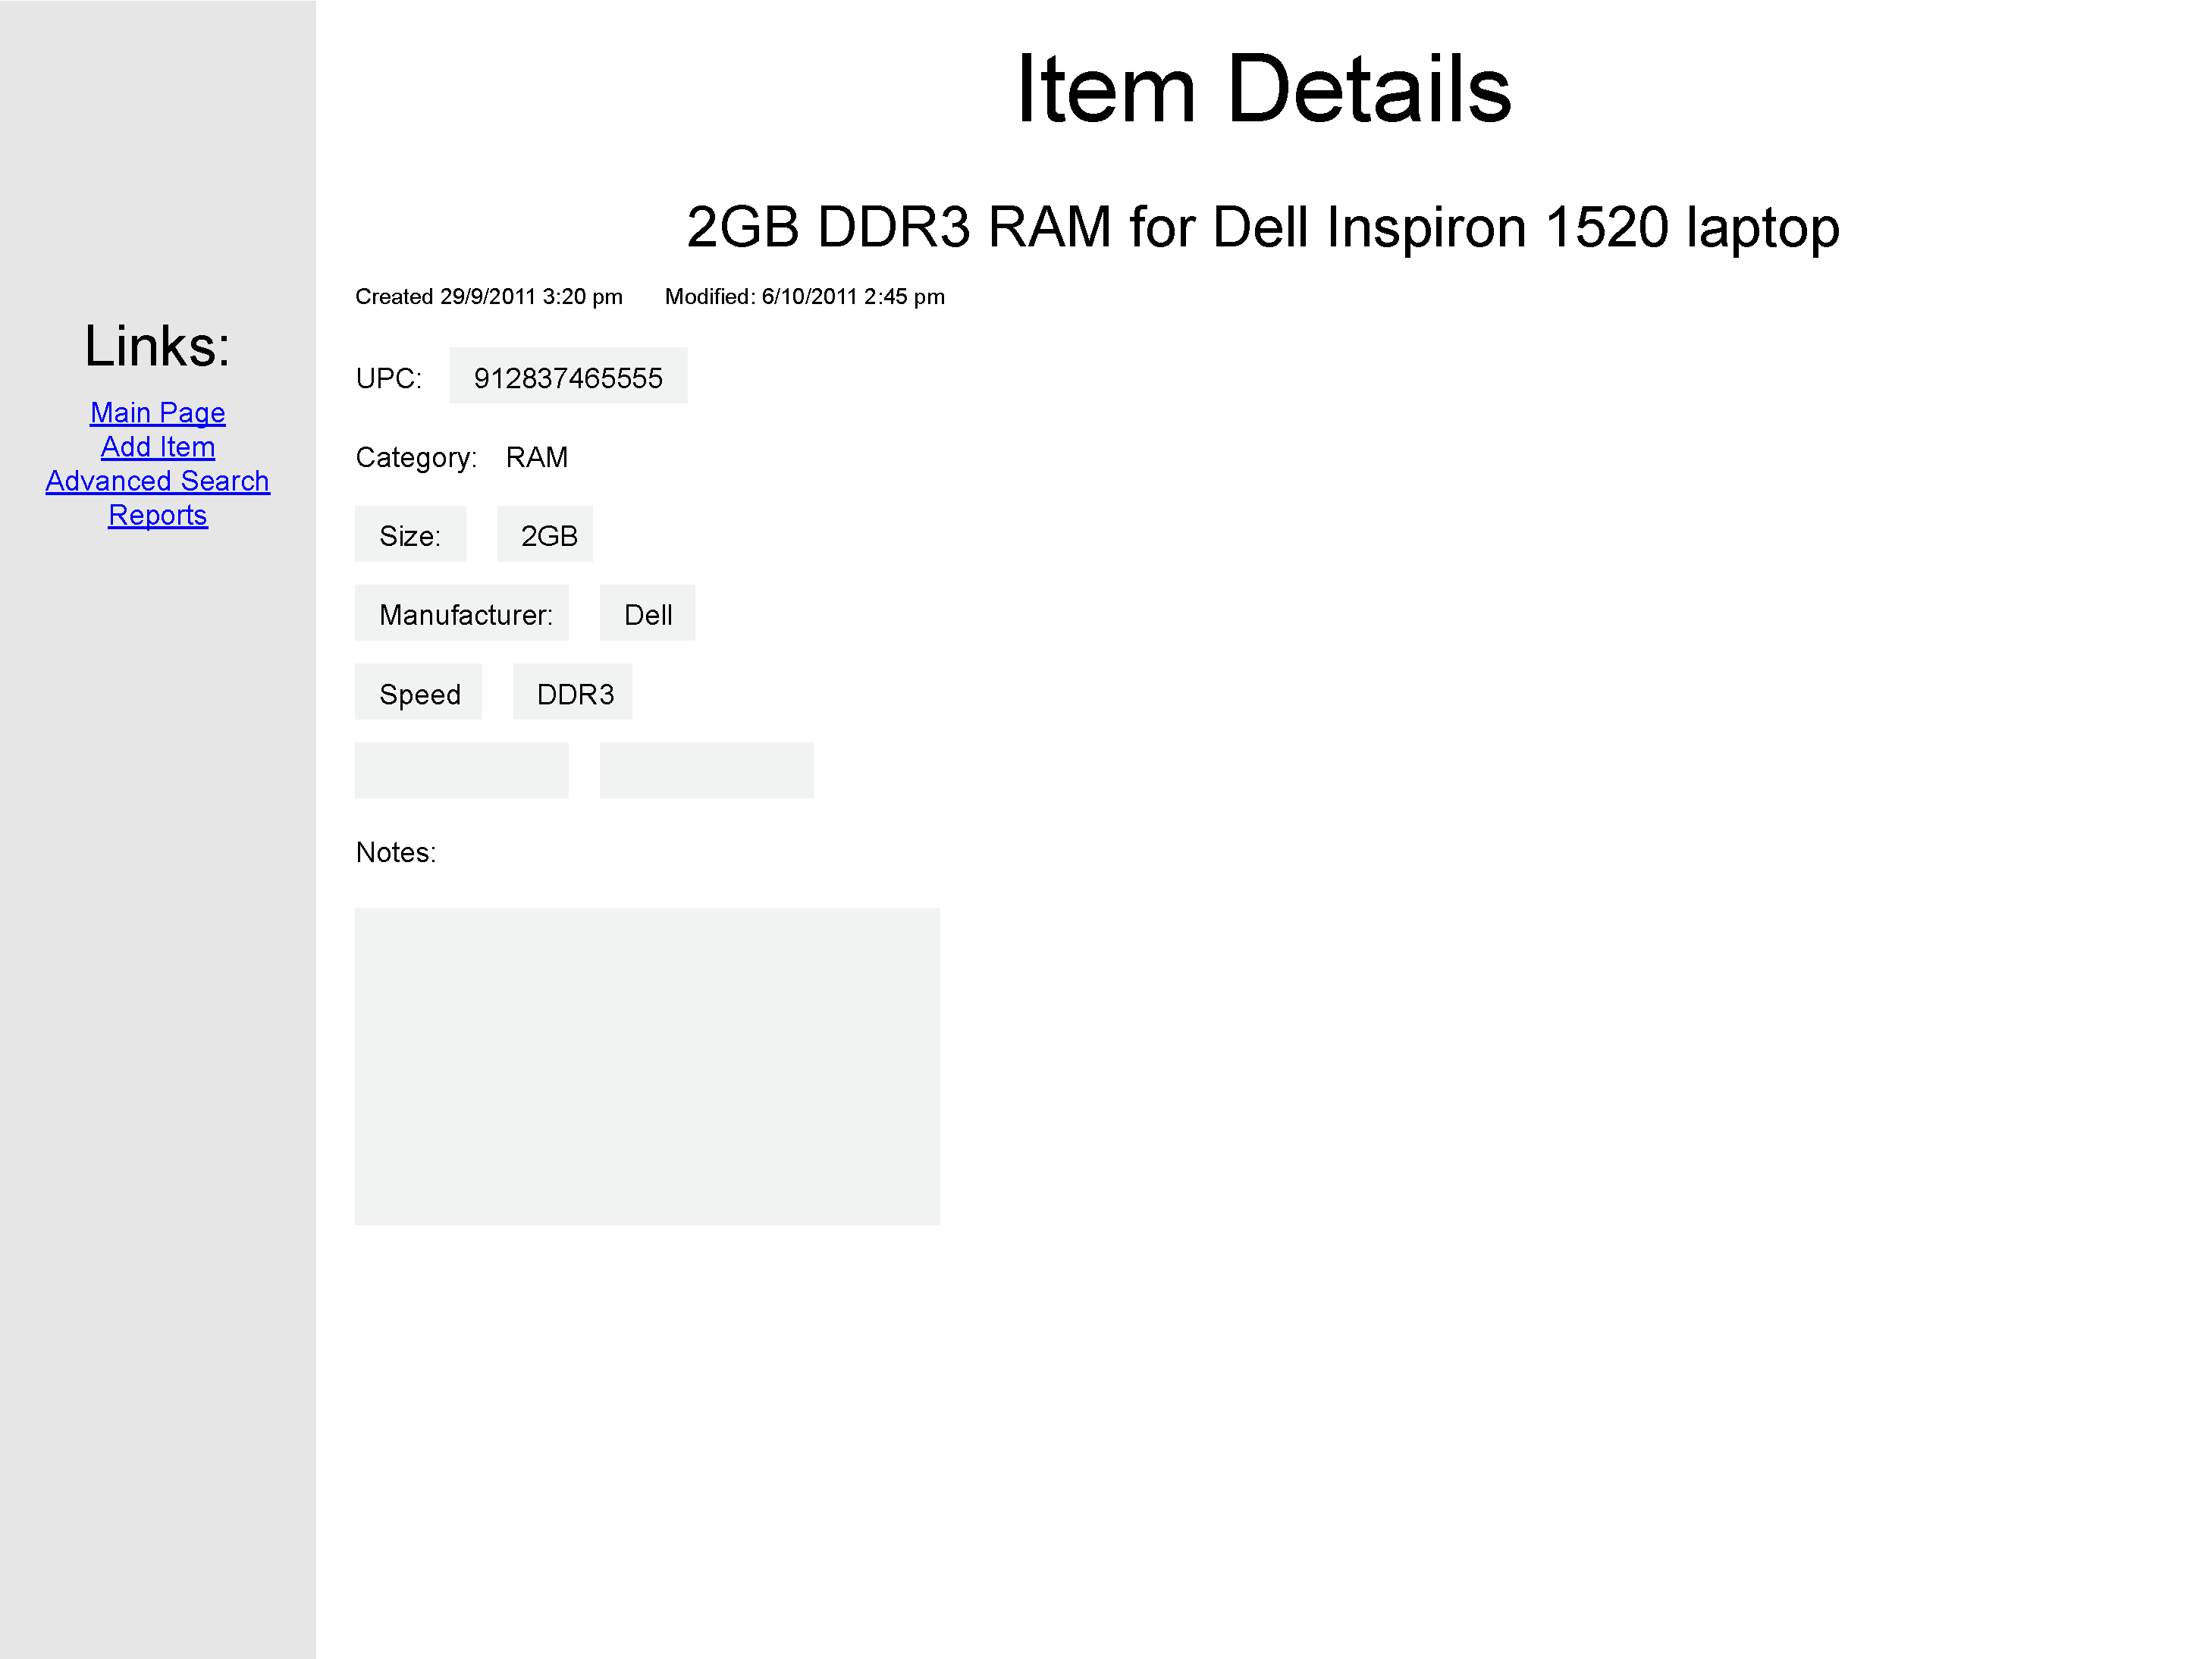
\includegraphics[keepaspectratio, width=4.5in]{modifyDetailsF0S4.pdf} \\
The item details page after the user has deselected the fields
\end{tabular}\\
~\\
~\\
\begin{tabular}{ p{4.5in} }
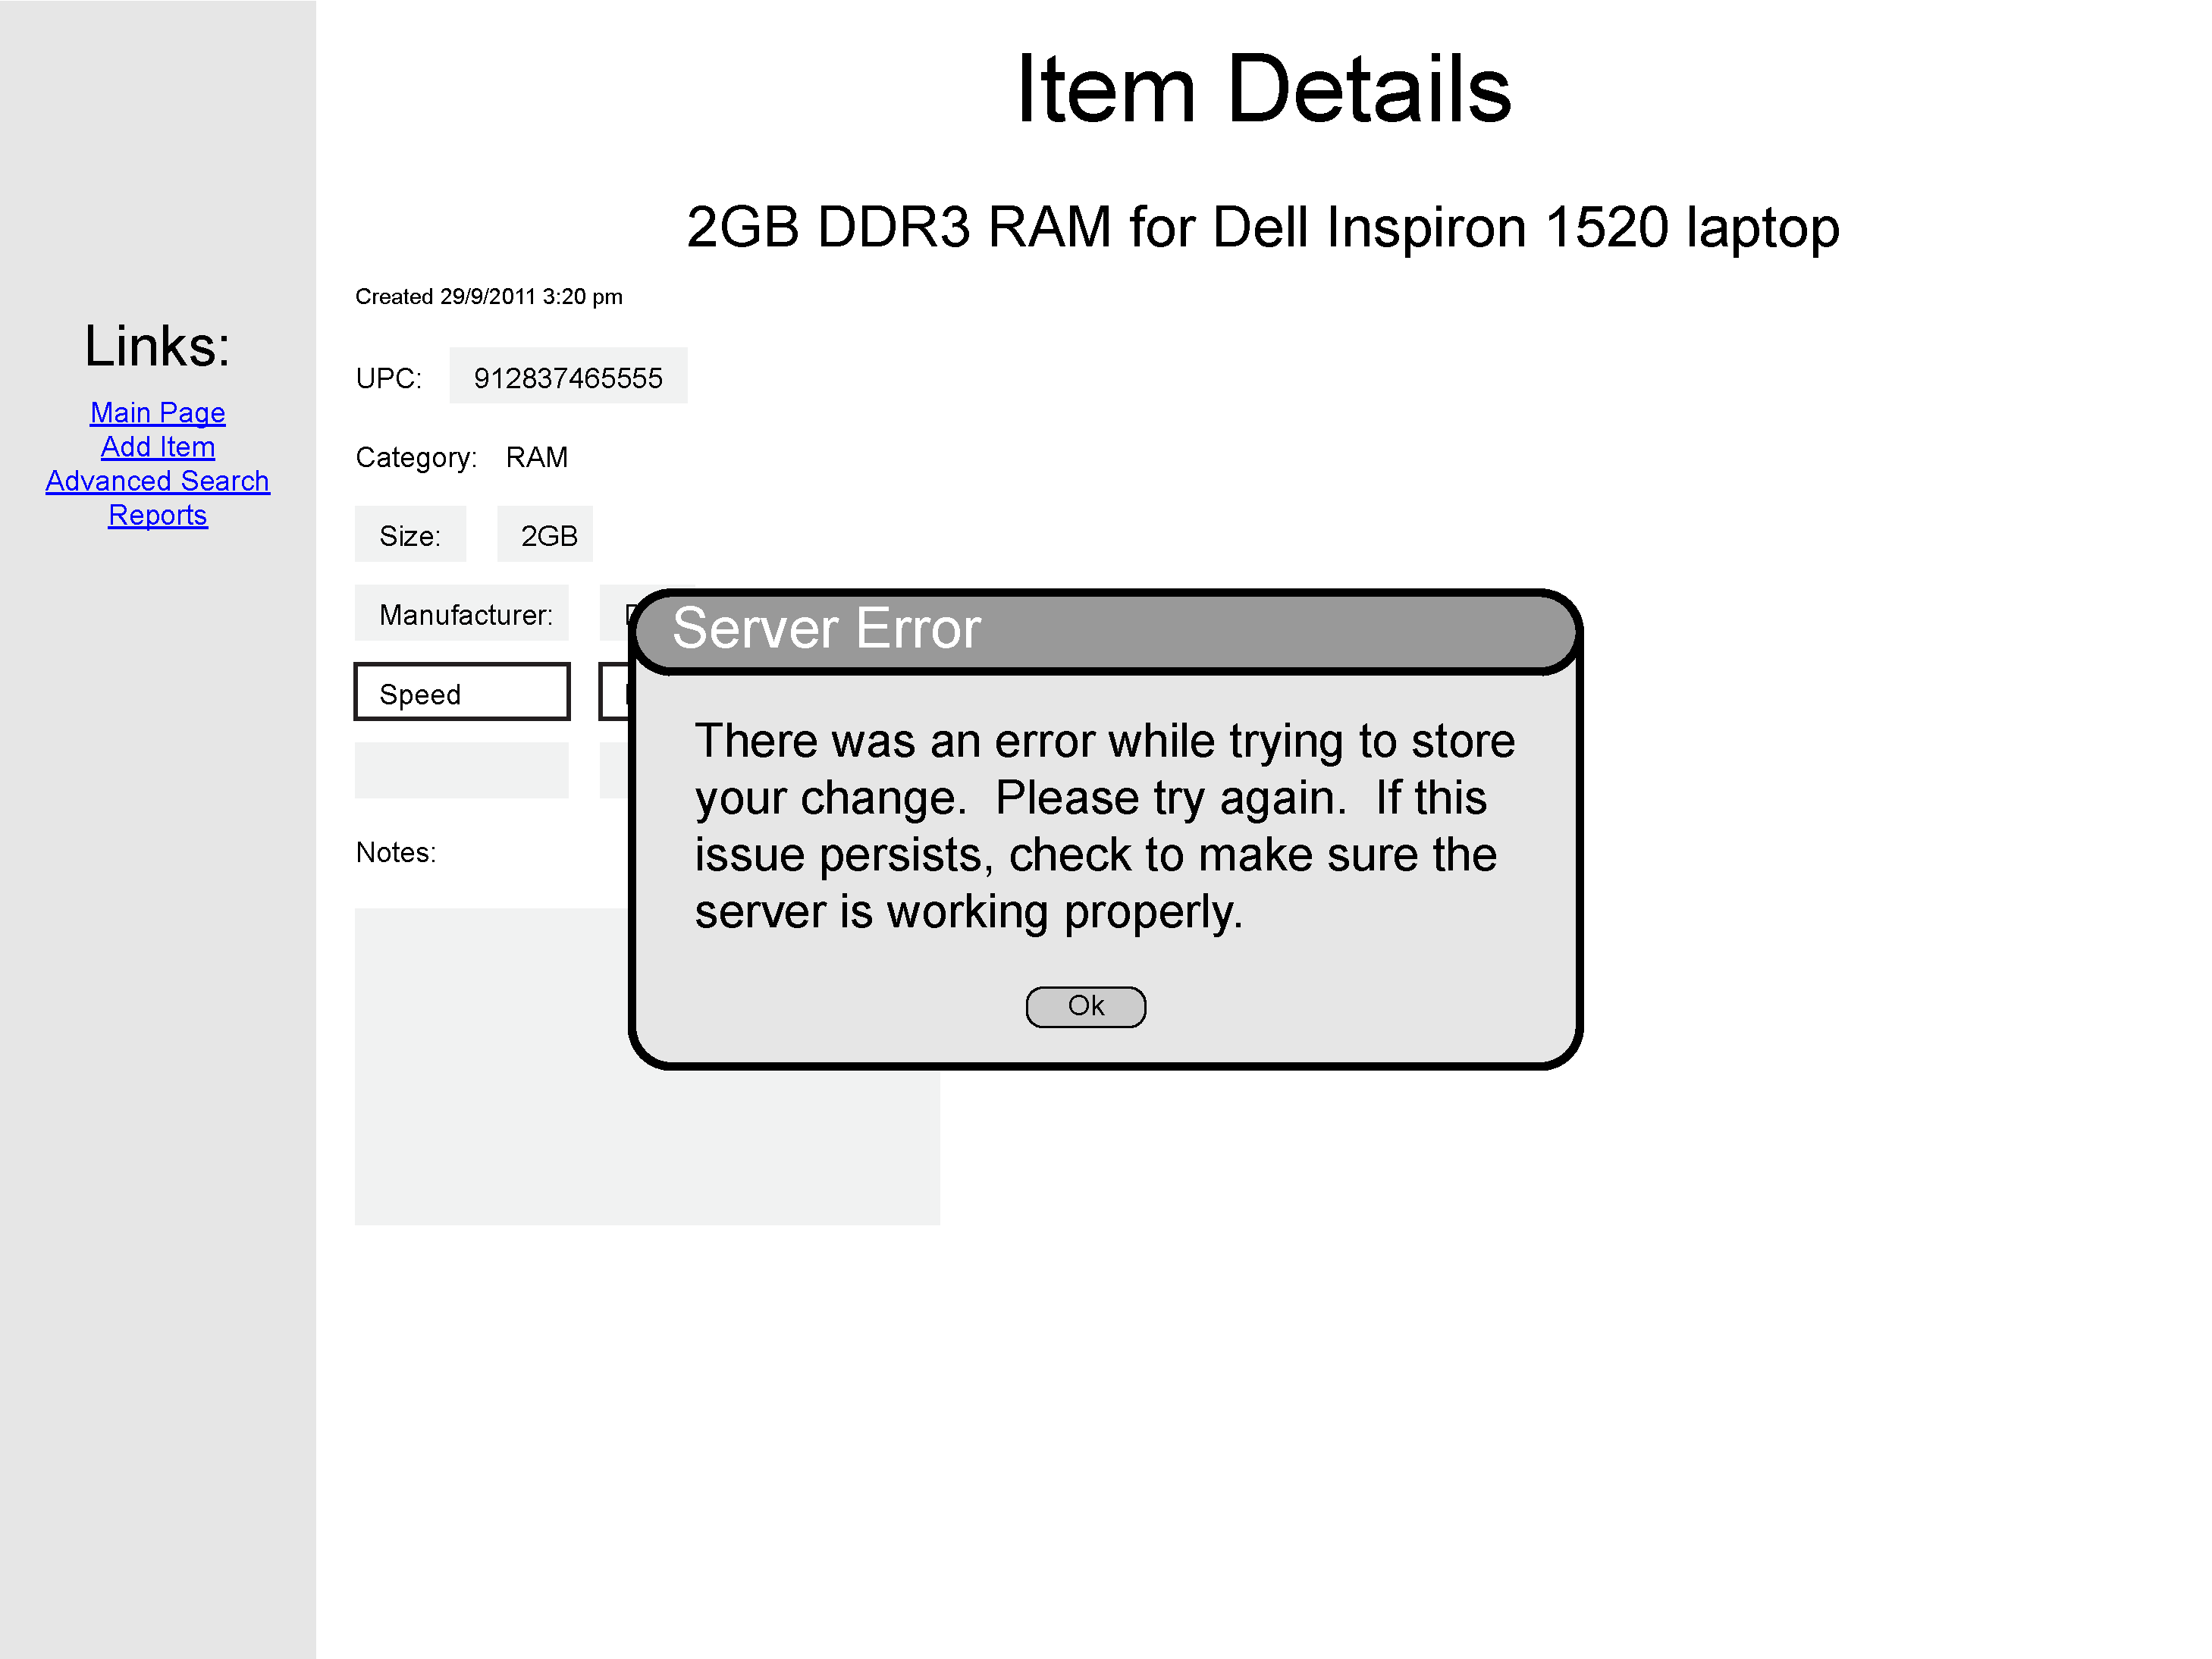
\includegraphics[keepaspectratio, width=4.5in]{modifyDetailsF1S4.pdf} \\
The item details page after the user has deselected the fields and the server has returned with an error
\end{tabular}\\
~\\
~\\
\begin{tabular}{ p{4.5in} }
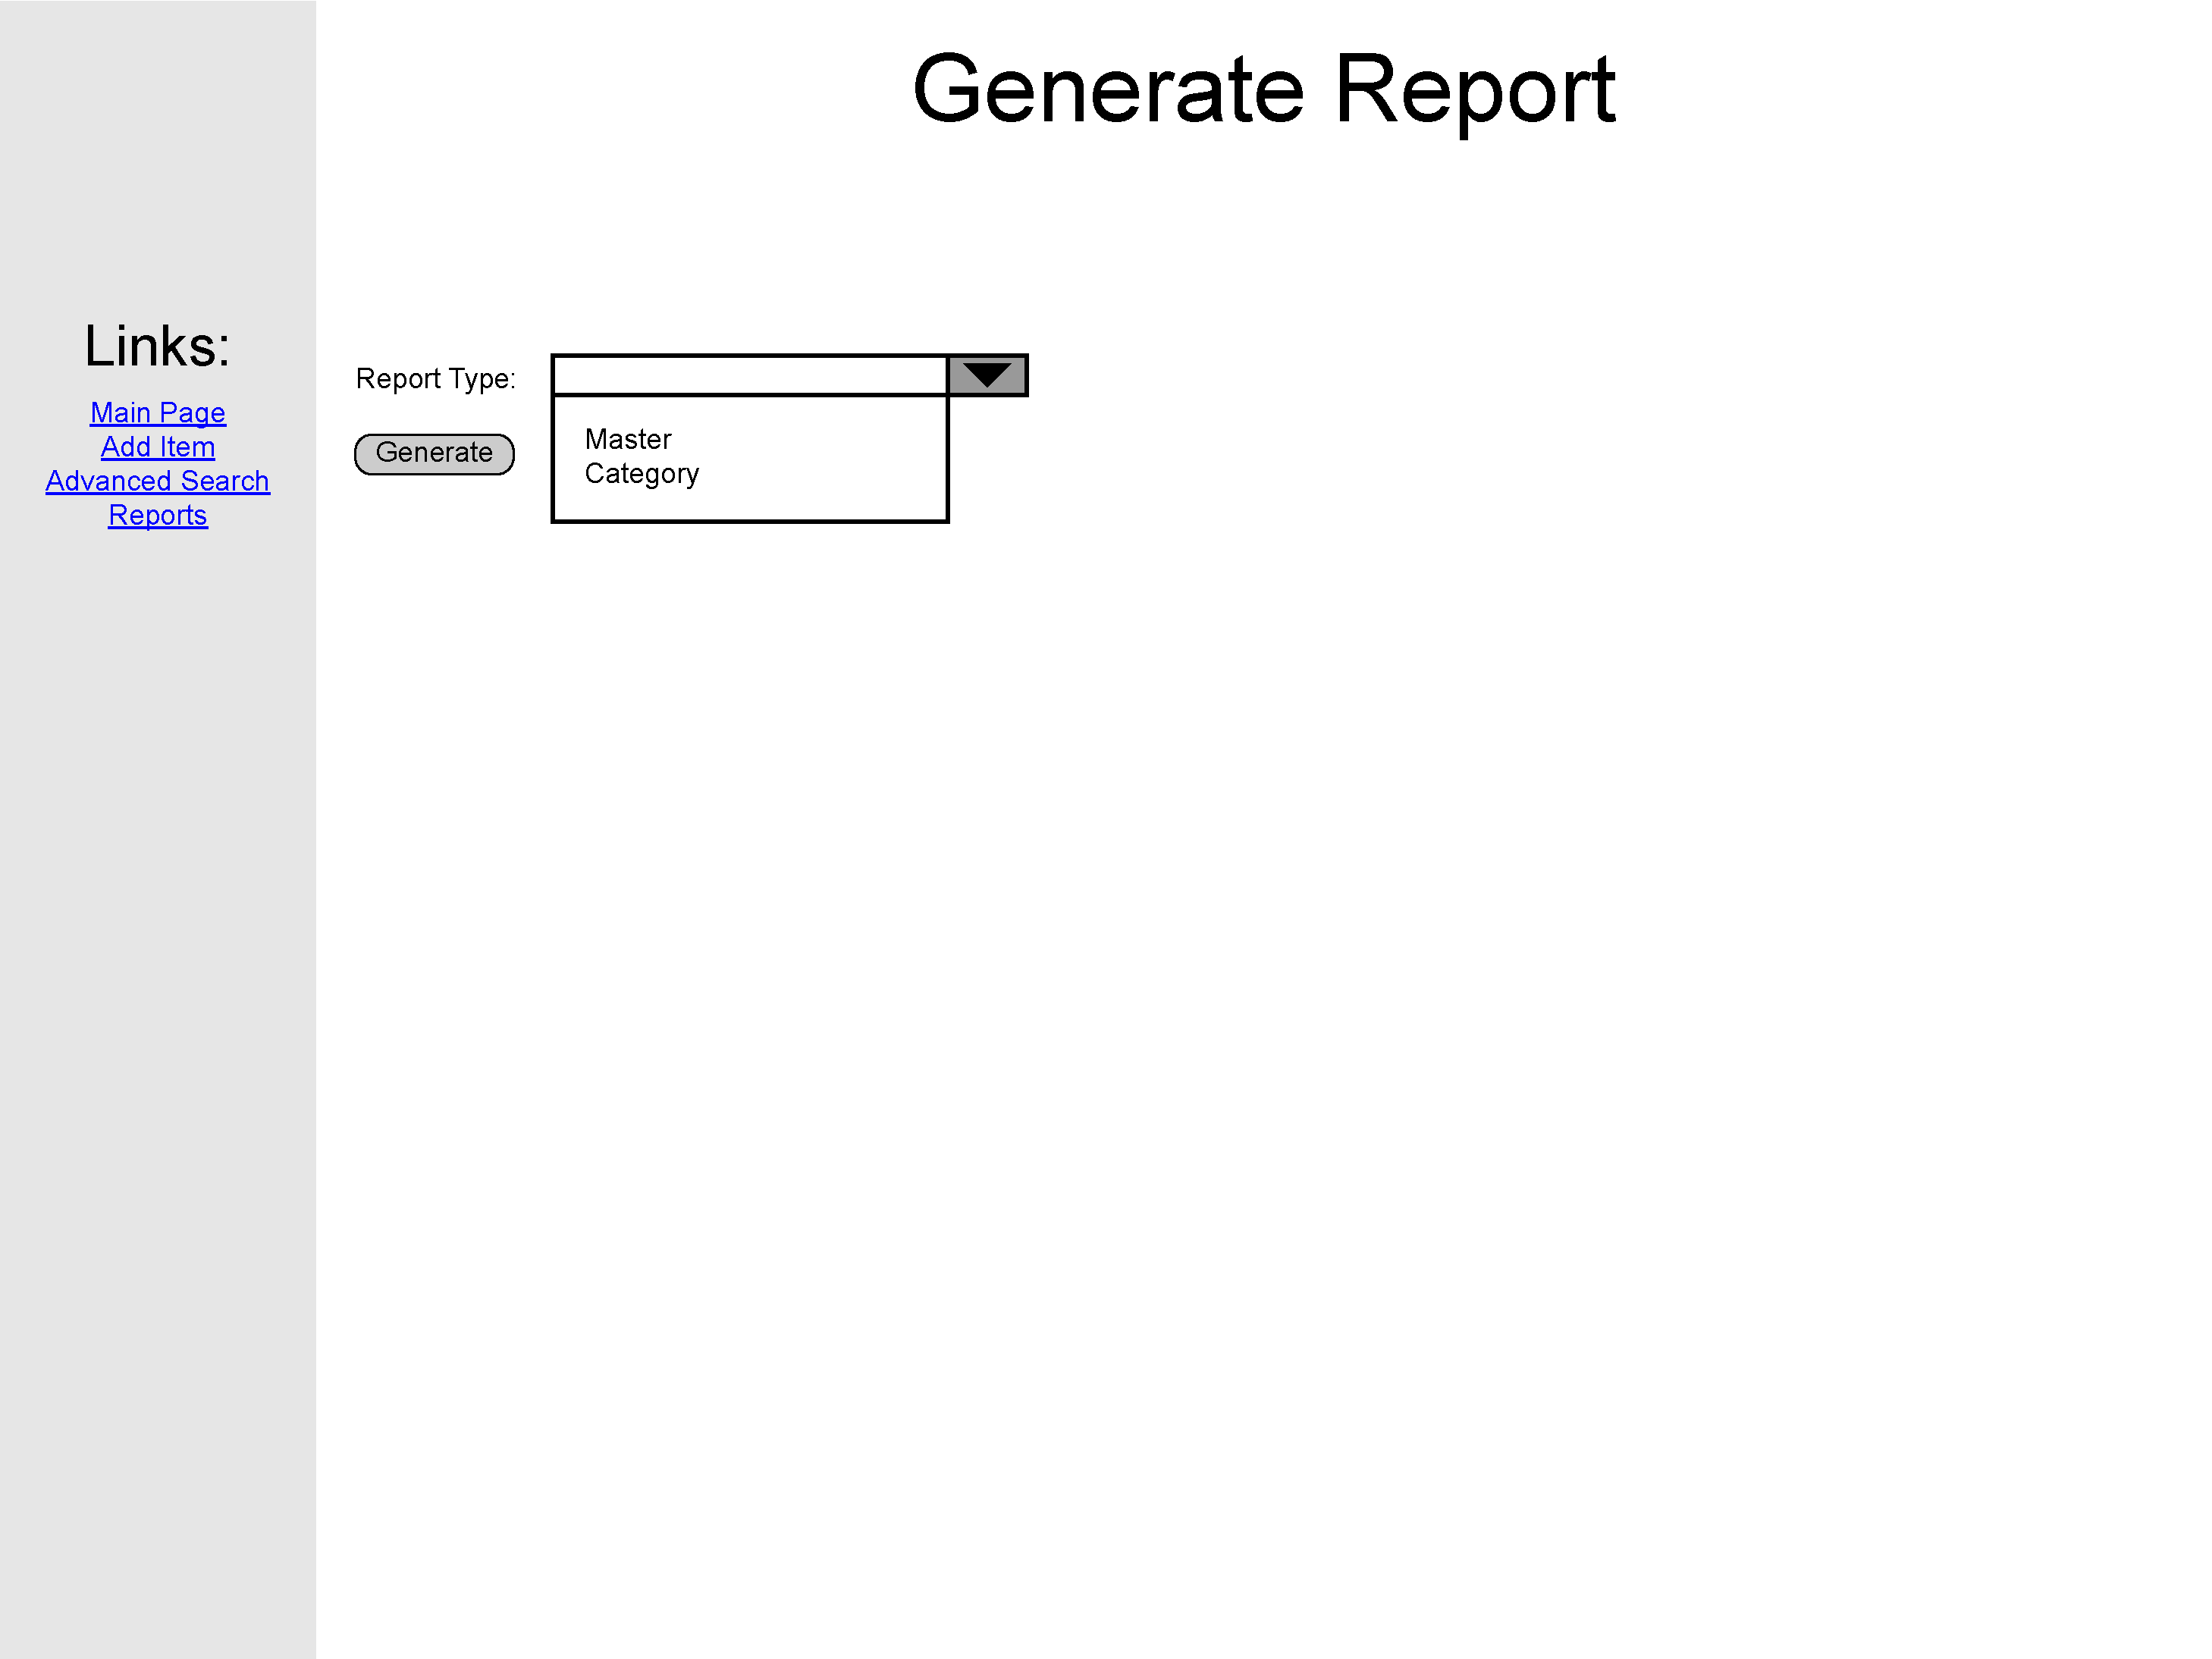
\includegraphics[keepaspectratio, width=4.5in]{generateReportF0S1.pdf} \\
The generate report page before a report type has been selected
\end{tabular}\\
~\\
~\\
\begin{tabular}{ p{4.5in} }
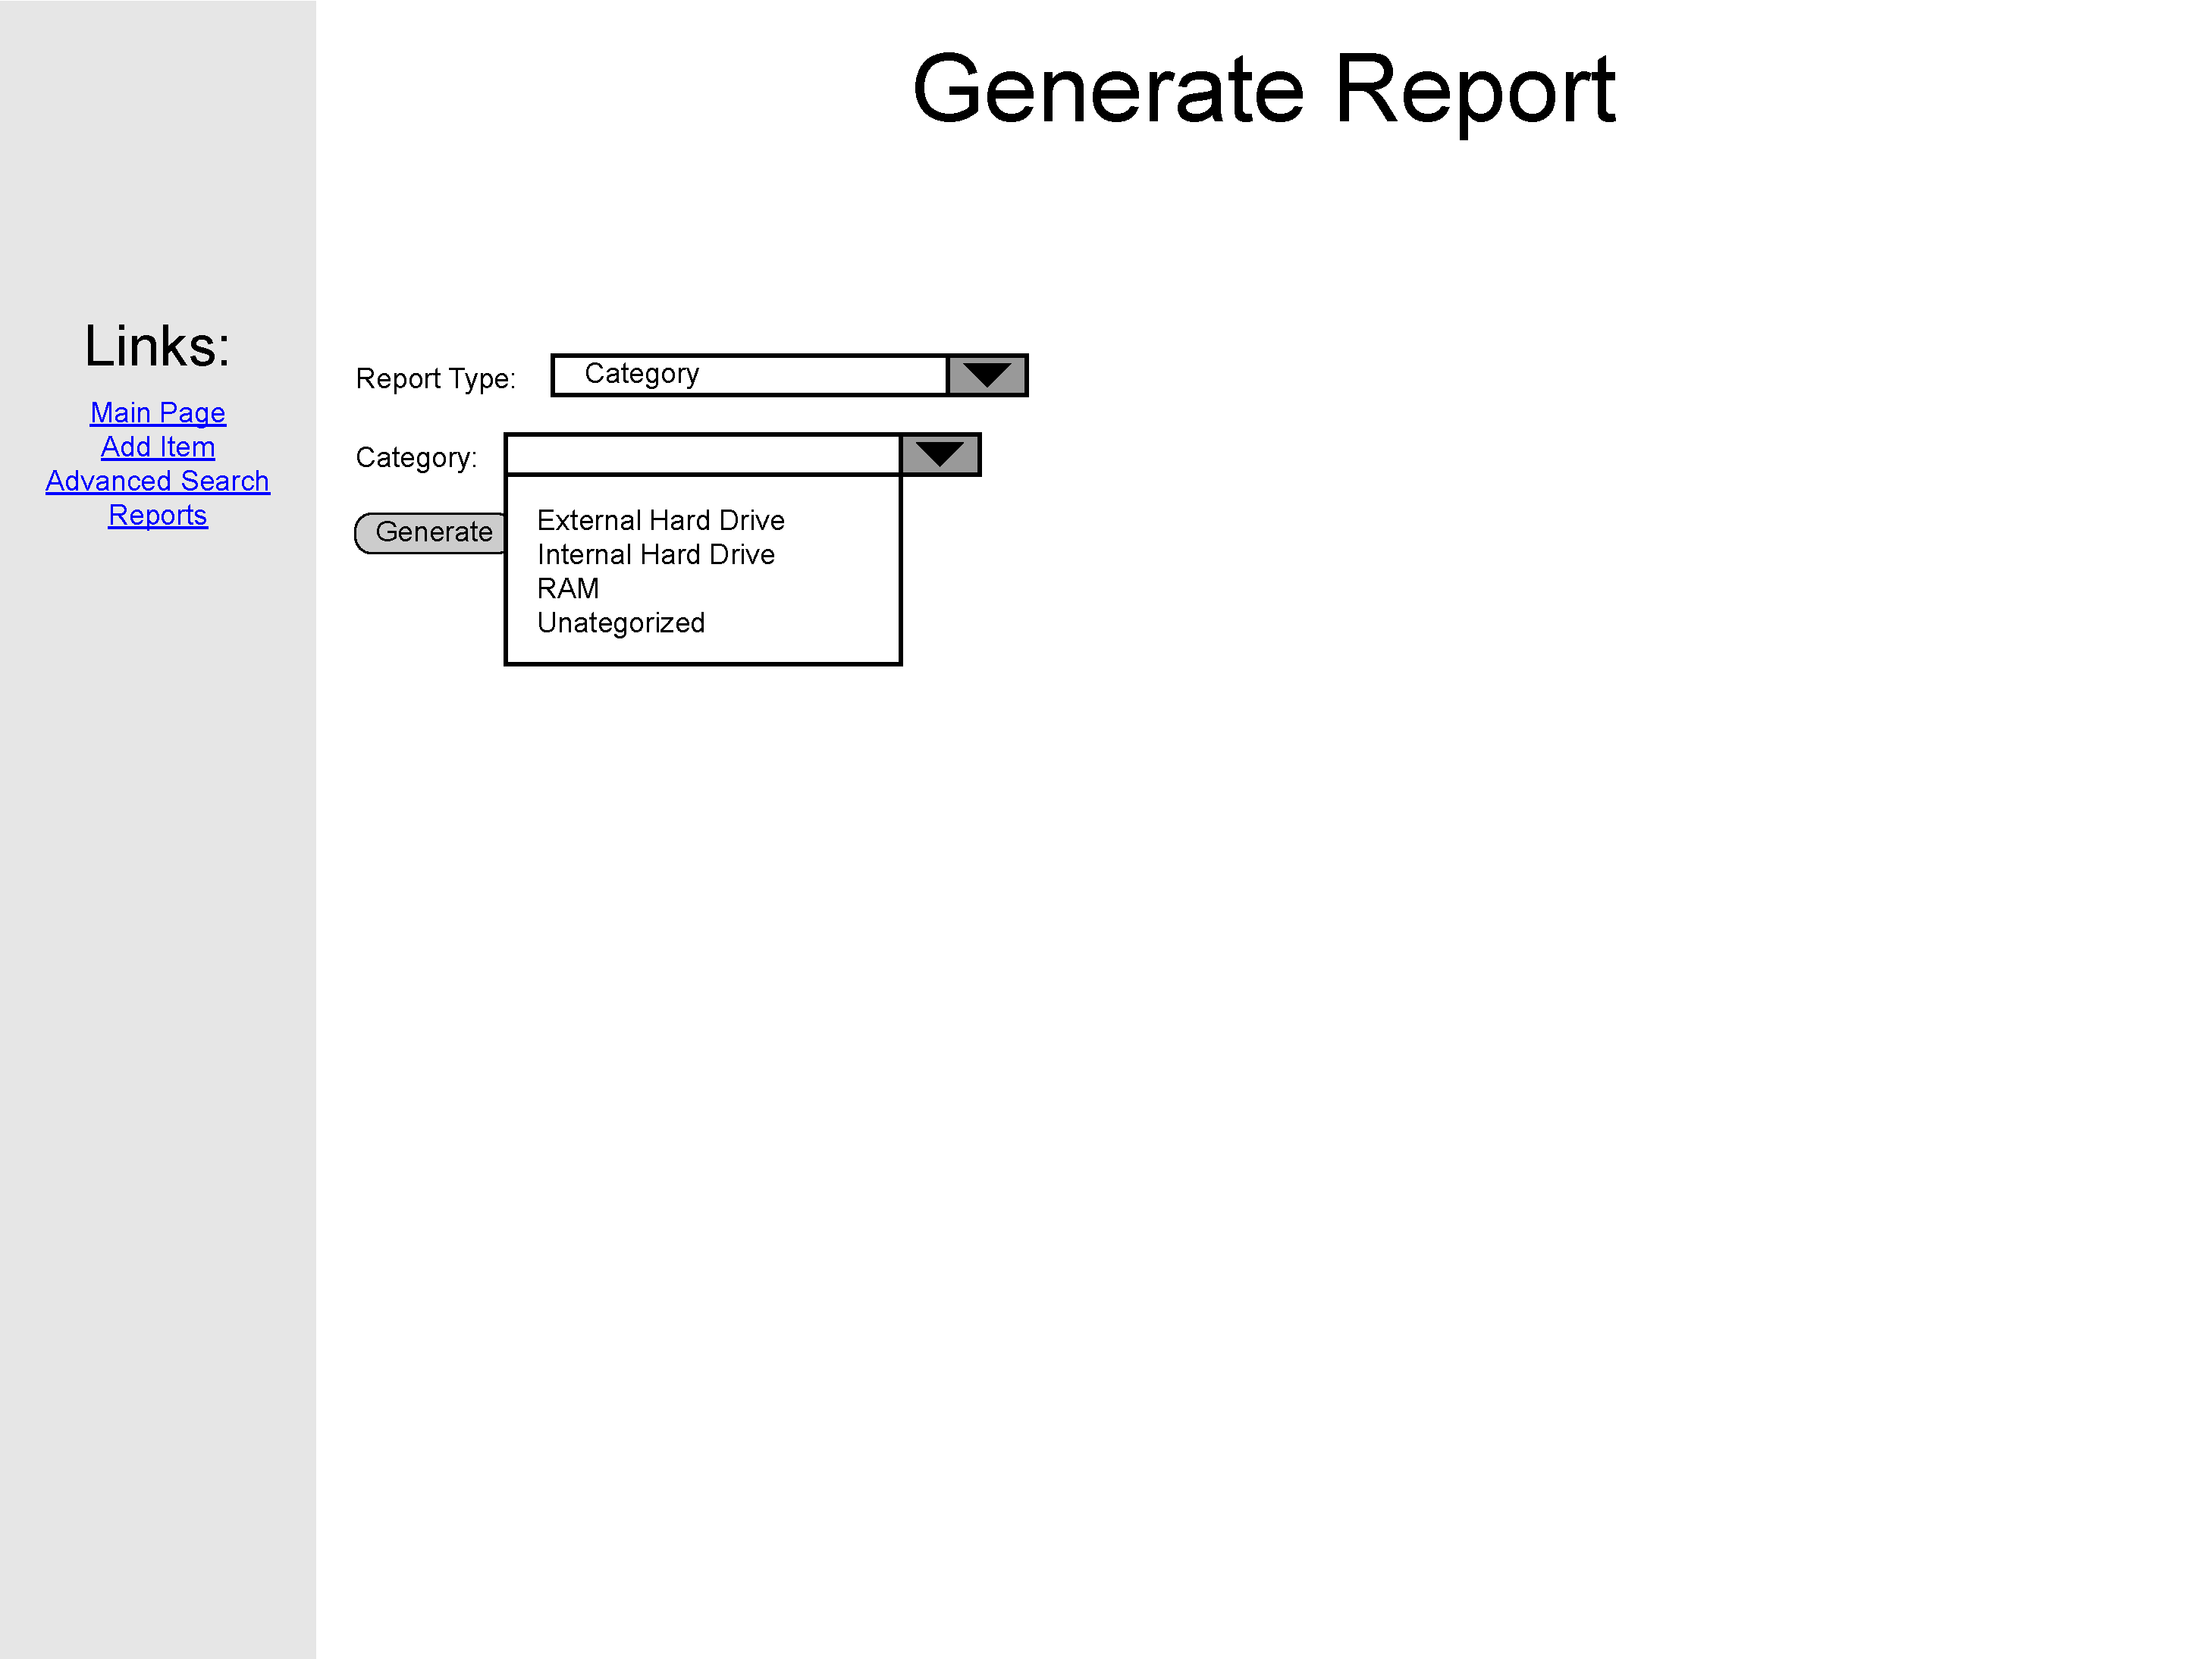
\includegraphics[keepaspectratio, width=4.5in]{generateReportF0S2.pdf} \\
The generate report page after the report type category has been selected, but before a category has been selected
\end{tabular}\\
~\\
~\\
\begin{tabular}{ p{4.5in} }
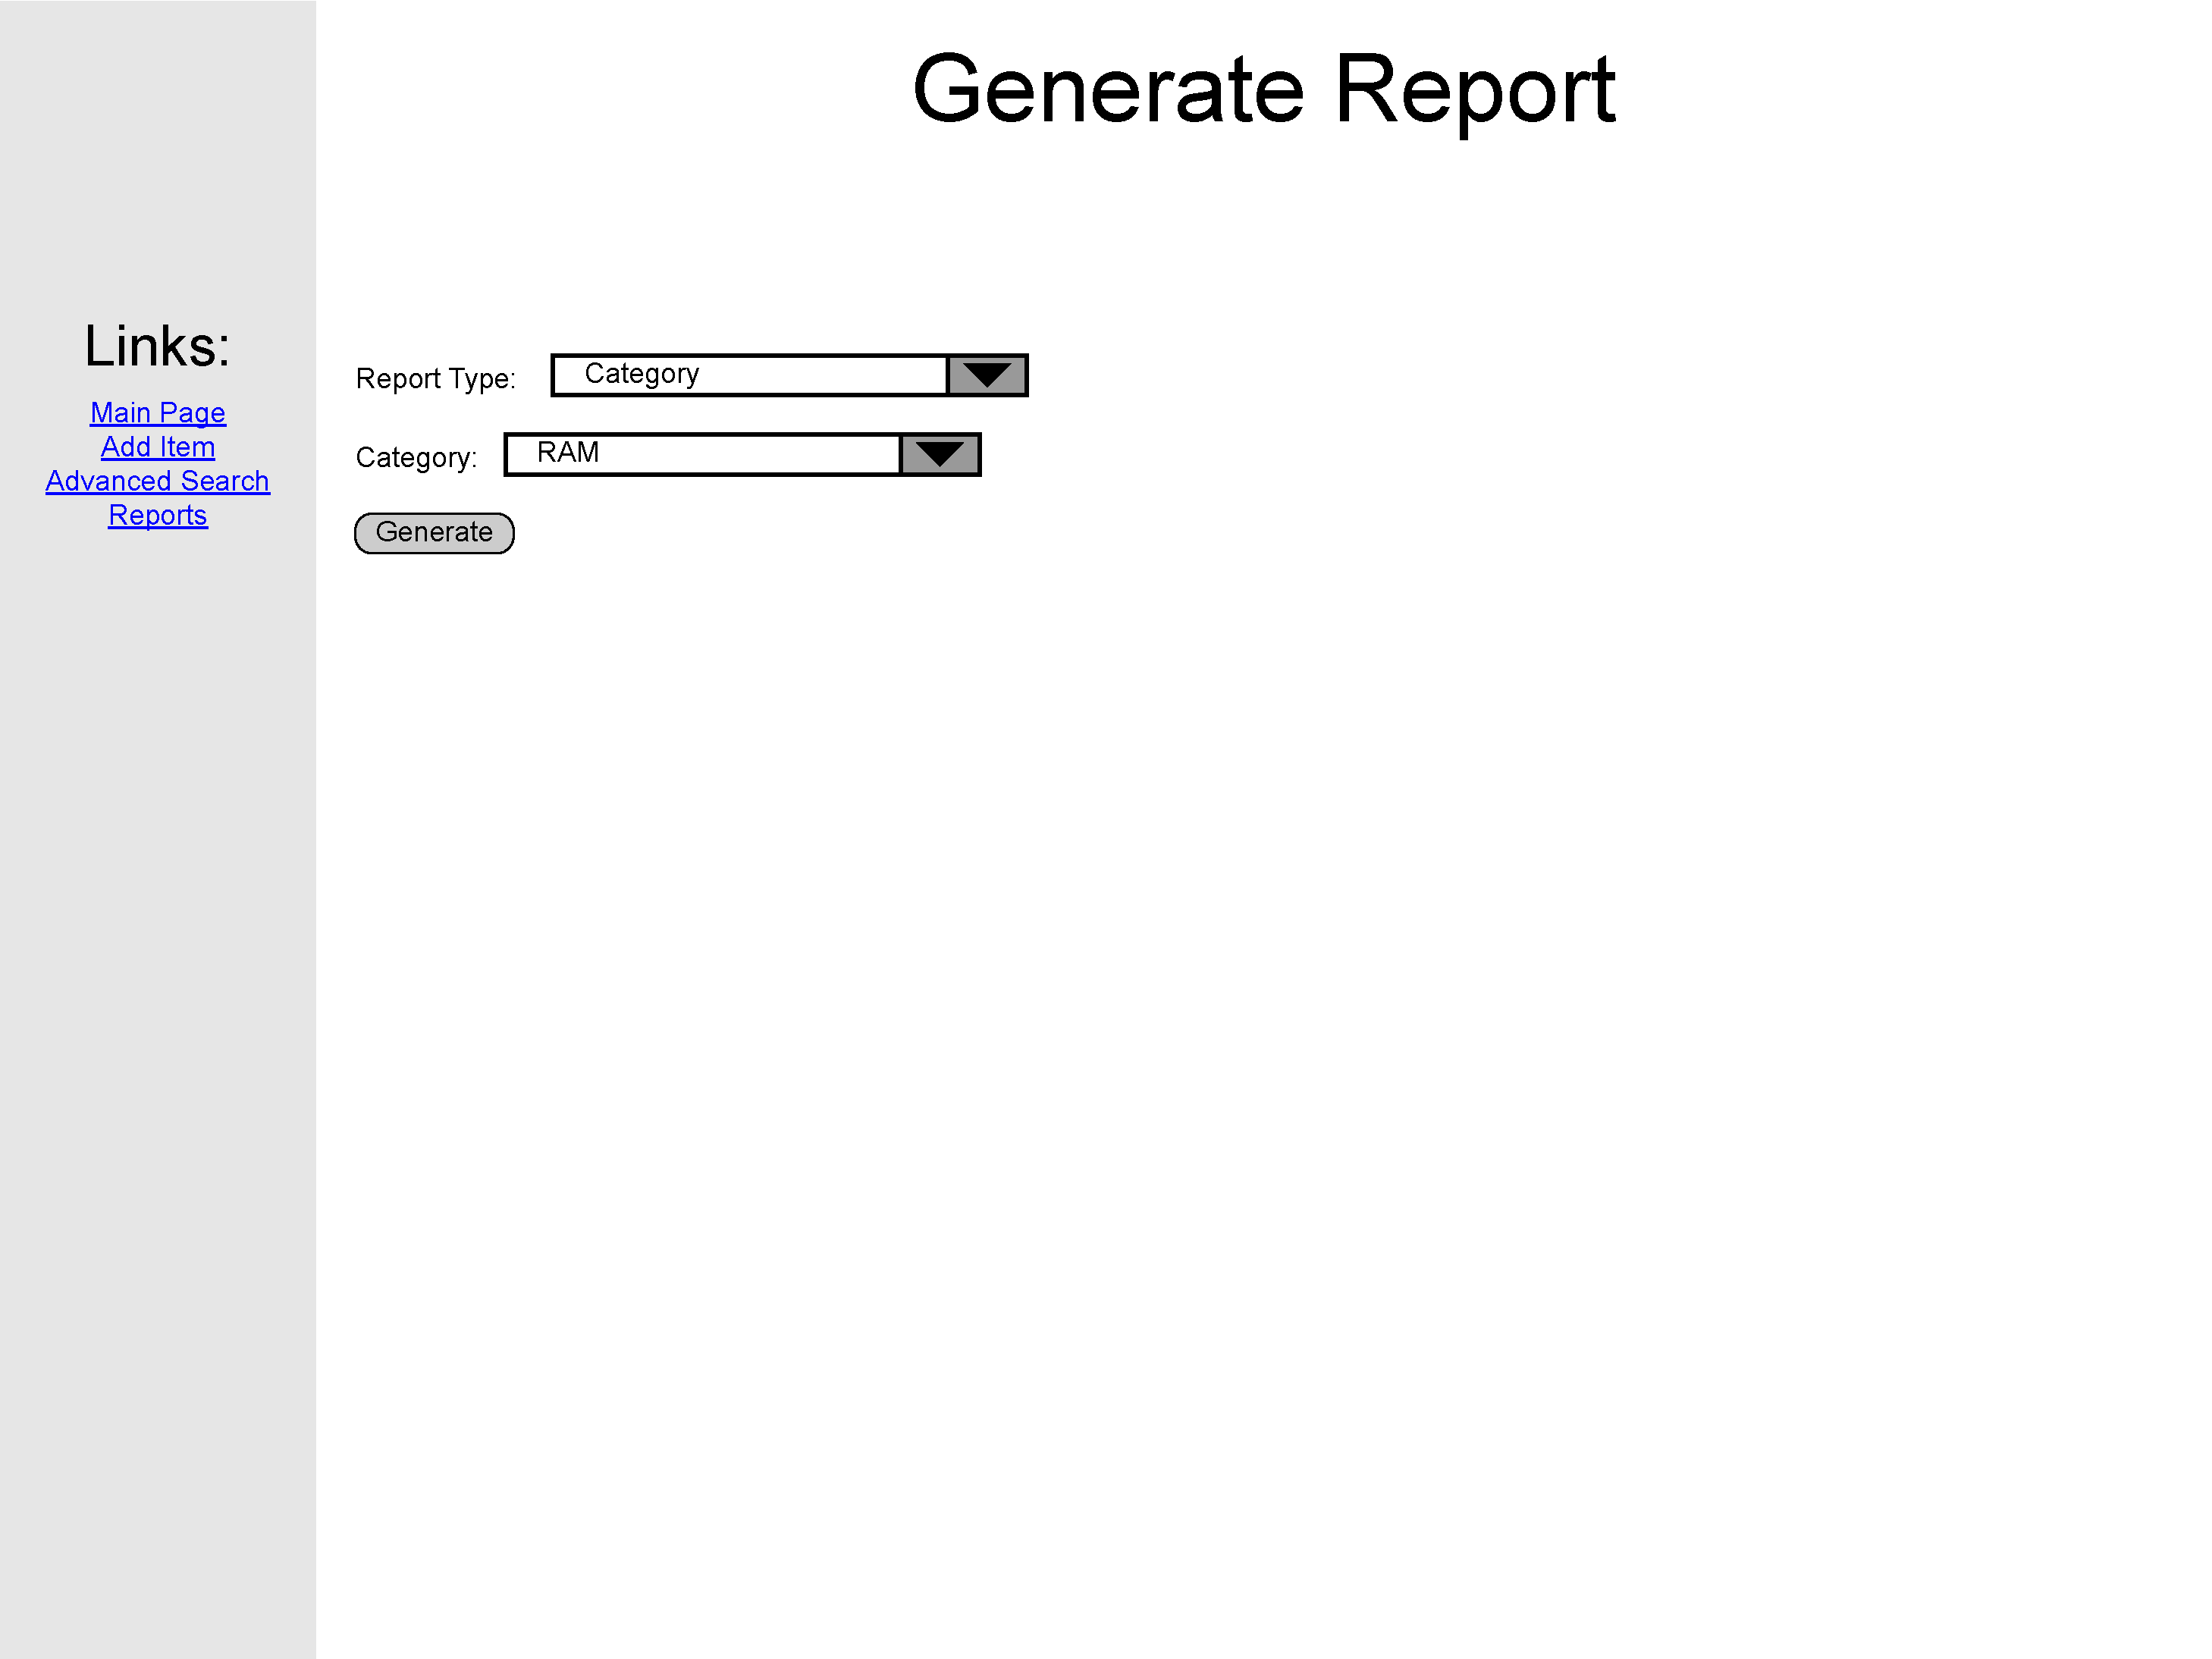
\includegraphics[keepaspectratio, width=4.5in]{generateReportF0S3.pdf} \\
The generate report page after the category of RAM has been selected
\end{tabular}\\
~\\
~\\
\begin{tabular}{ p{4.5in} }
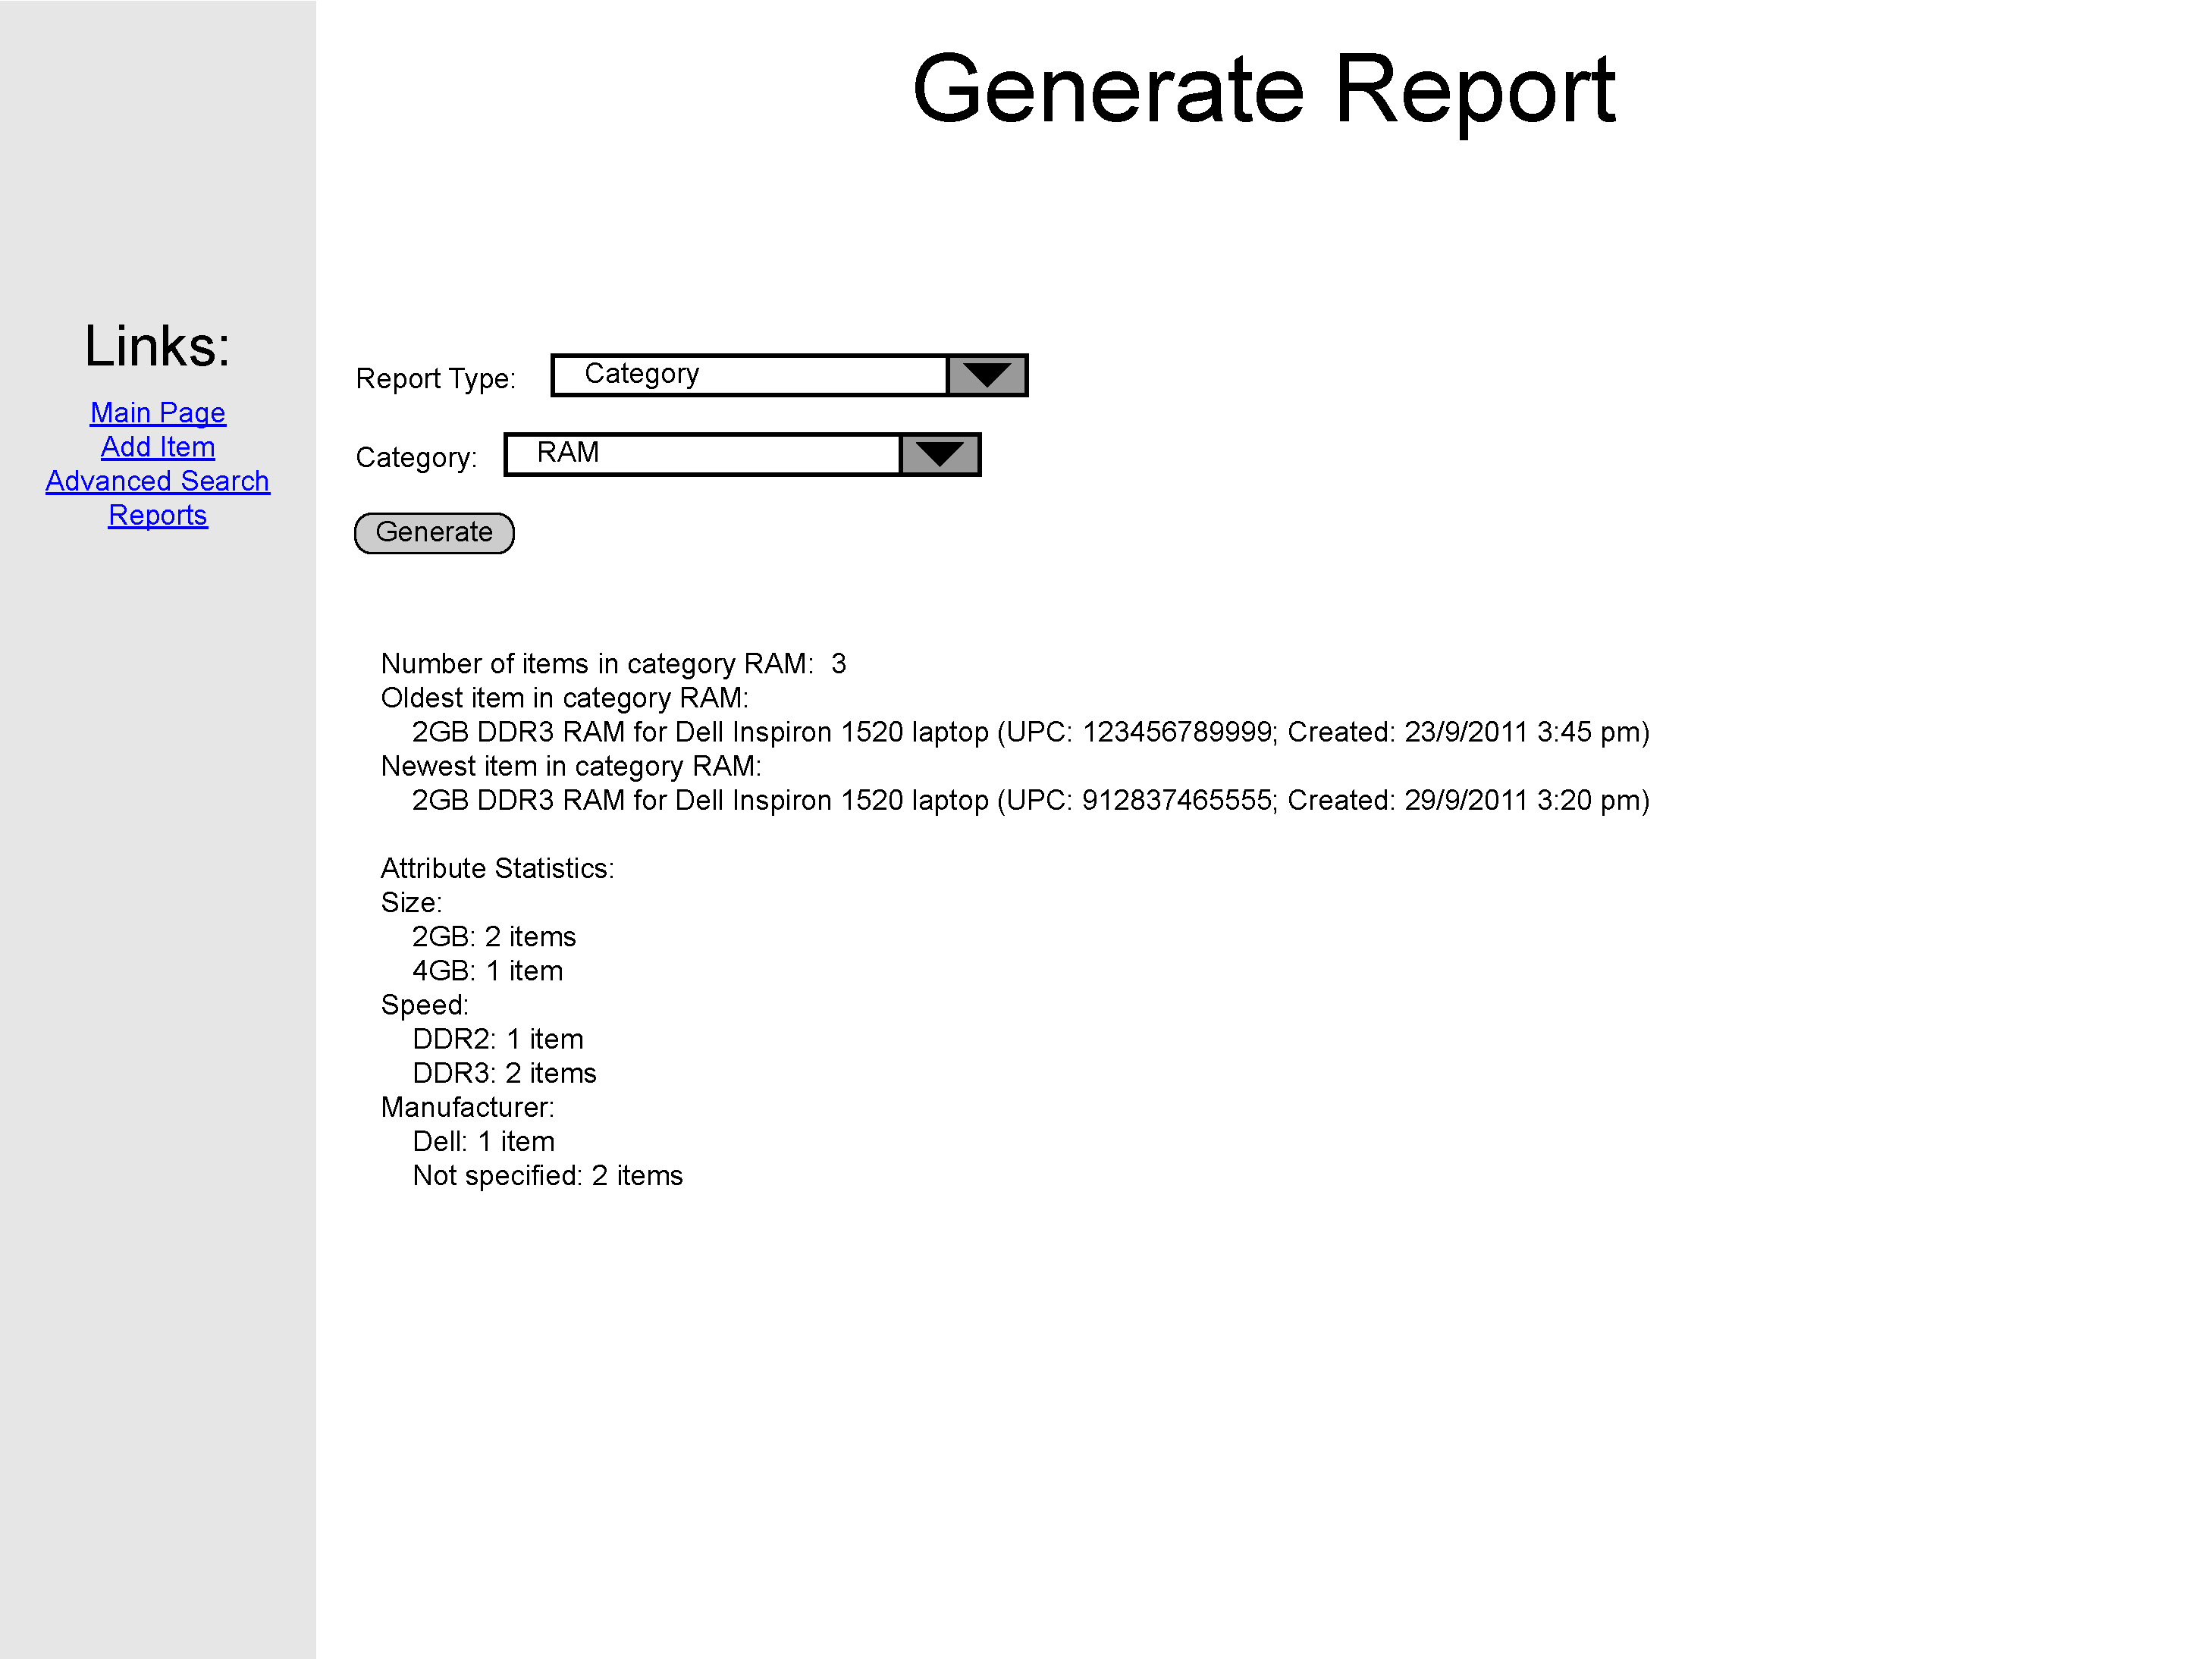
\includegraphics[keepaspectratio, width=4.5in]{generateReportF0S4.pdf} \\
The generate report page with the report being displayed
\end{tabular}

\section{Index and Glossary}
\textbf{Bug}: An error in a computer program. A critical bug is a bug that strongly affects important parts of a system (\pageref{bug}).\\ \\
\textbf{Data corruption}: Errors in data that introduce unintended changes to the data (\pageref{data_corruption}).\\ \\
\textbf{Degraded system}: The system becomes degraded if there are too many queries performed too quickly or if the amount of data needing to be searched through becomes too large. When the system is degraded, it may result in the system ceasing to function and requiring a reboot (\pageref{degrad_sys}).\\ \\
\textbf{Interface}: A point of interaction between systems, whether hardware or software, that allows the systems to communicate using some protocol (\pageref{interface}).\\ \\
\textbf{Performance}: The speed and efficiency of an operation, program, or system at a set of tasks (\pageref{performance}).\\ \\
\textbf{Reliability}: The ability of a system to function in a range of conditions for a period of time without failing to perform its tasks (\pageref{reliability}).\\ \\
\textbf{REST}: Stands for ``Representational state transfer;'' is a style software architecture often used in servers for simplicity and scalability. Amongst other aspects of REST, it is stateless. This means each request sent from the client of the server that uses REST to the server does not require any information from any previous requests. All information required to fulfill the request must be sent with the request (\pageref{rest}).\\ \\
\textbf{SOAP}: Stands for ``Simple Object Access Protocol;'' is a protocol for exchanging structured information across a network (\pageref{soap}).\\ \\
\textbf{Supportability}: The ease with which a system can be fixed should it become broken or out of order (\pageref{support}).\\ \\
\textbf{Usability}: The ease with which one may use or learn to use a system (\pageref{usability}).

\section{References}
\hangindent=1.4cm
\textbf{(1)} Leffingwell, Dean, and Don Widrig.
\emph{Managing Software Requirements: a Use Case Approach}.
Addison-Wesley, Boston,
2nd Edition,
2003.\\

\noindent\hangindent=1.4cm
\textbf{(2)} ``Ruby 1.9.2''
\emph{Download Ruby.} Ruby. Web.  6 October 2011. \\

\noindent\hangindent=1.4cm
\textbf{(3)} ``Sinatra 1.3.0''
\emph{Sinatra: Documentation.} Sinatra. Web.  6 October 2011.\\

\noindent\hangindent=1.4cm
\textbf{(4)} ``Ubuntu 11.04''
\emph{Download Ubuntu.} Ubuntu. Web.  6 October 2011.\\

\noindent\hangindent=1.4cm
\textbf{(5)} ``SQLite 3.7.8''
\emph{SQLite Download Page.} SQLite. Web.  6 October 2011.\\

\noindent\hangindent=1.4cm
\textbf{(6)} ``Cucumber 1.1.0''
\emph{cucumber/cucumber.} Cucumber. Web.  6 October 2011.\\

\noindent\hangindent=1.4cm
\textbf{(7)} ``RSpec 2.6.0''
\emph{RSpec Documentation.} Relish. Web.  6 October 2011.\\

\noindent\hangindent=1.4cm
\textbf{(8)} ``DataMapper 1.1.0''
\emph{DataMapper - Documentation.} DataMapper. Web.  6 October 2011.\\

\noindent\hangindent=1.4cm
\textbf{(9)} ``Google Chrome 14.0.8'' 
\emph{About Google Chrome.} Google. Web.  7 October 2011.\\

\noindent\hangindent=1.4cm
\textbf{(10)} ``Firefox 7.0.1''
\emph{Mozilla Firefox Web Browser - Free Download.} Mozilla. Web.  7 October 2011.\\

\noindent\hangindent=1.4cm
\textbf{(11)} ``Apache 2.2''
\emph{Apache HTTP Server Version 2.2 Documentation - Apache HTTP Server.} Apache. Web.  7 October 2011.\\

\end{document}